%%%%%%%%%%%%%%%%%%%%%%%%%%%%%%%%%%%%%%%%%%%%%%%%%%%%%%%%%%%%%%%%%%%%%%%%%%%%%%%%
%% MASTER'S THESIS                                                            %%
%%                                                                            %% 
%% Title (en): Mining Parallel Corpora from the Web                           %%
%% Title (sk): Rafinácia paralelných korpusov z webu                          %%
%%                                                                            %%
%% Author: Bc. Jakub Kúdela                                                   %%
%% Supervisor: Doc. RNDr. Irena Holubová, Ph.D.                               %%
%% Consultant: RNDr. Ondřej Bojar, Ph.D.                                      %%
%%                                                                            %%
%% Academic year: 2015/2016                                                   %%
%%%%%%%%%%%%%%%%%%%%%%%%%%%%%%%%%%%%%%%%%%%%%%%%%%%%%%%%%%%%%%%%%%%%%%%%%%%%%%%%

%%%%%%%%%%%%%%%%%%%%%%%%%%%%%%%%%%%%%%%%%%%%%%%%%%%%%%%%%%%%%%%%%%%%%%%%%%%%%%%%
%% Document Class                                                             %%
%%%%%%%%%%%%%%%%%%%%%%%%%%%%%%%%%%%%%%%%%%%%%%%%%%%%%%%%%%%%%%%%%%%%%%%%%%%%%%%%

\documentclass[12pt,a4paper]{report} % One-sided printing
%\documentclass[12pt,a4paper,twoside,openright]{report} % Two-sided printing

%% Page Layout %%%%%%%%%%%%%%%%%%%%%%%%%%%%%%%%%%%%%%%%%%%%%%%%%%%%%%%%%%%%%%%%%

\setlength{\textwidth}{145mm}
\setlength{\textheight}{247mm}
\setlength{\oddsidemargin}{15mm}
\setlength{\evensidemargin}{15mm} % One-sided printing
%\setlength{\evensidemargin}{0mm} % Two-sided printing
\setlength{\topmargin}{0mm}
\setlength{\headsep}{0mm}
\setlength{\headheight}{0mm}

%% Paragraph Formatting %%%%%%%%%%%%%%%%%%%%%%%%%%%%%%%%%%%%%%%%%%%%%%%%%%%%%%%%

\setlength{\parindent}{0mm}
\setlength{\parskip}{5mm}

\clubpenalty=10000 % Extra penalty for breaking after first line of a paragraph
\widowpenalty=10000 % Extra penalty for breaking before last line of a paragraph

%% Alias Definitions %%%%%%%%%%%%%%%%%%%%%%%%%%%%%%%%%%%%%%%%%%%%%%%%%%%%%%%%%%%

%\let\openright=\clearpage % One-sided printing
\let\openright=\cleardoublepage % Two-sided printing

%%%%%%%%%%%%%%%%%%%%%%%%%%%%%%%%%%%%%%%%%%%%%%%%%%%%%%%%%%%%%%%%%%%%%%%%%%%%%%%%
%% Packages                                                                   %%
%%%%%%%%%%%%%%%%%%%%%%%%%%%%%%%%%%%%%%%%%%%%%%%%%%%%%%%%%%%%%%%%%%%%%%%%%%%%%%%%

%% Encoding and multilingual support %%%%%%%%%%%%%%%%%%%%%%%%%%%%%%%%%%%%%%%%%%%

% Accept different input encodings.
\usepackage[utf8]{inputenc}

%% Standard package for selecting font encodings.
\usepackage[T1]{fontenc}

% Multilingual support for Plain TeX or LaTeX.
\usepackage[english,slovak]{babel}

\usepackage{aeguill}

%% Formatting %%%%%%%%%%%%%%%%%%%%%%%%%%%%%%%%%%%%%%%%%%%%%%%%%%%%%%%%%%%%%%%%%%

\usepackage{verbatim}

%% Flexible and complete interface to document dimensions.
%\usepackage[left=4cm]{geometry}

%% "Wide" a4 layout.
%\usepackage{a4wide}

%% Graphics %%%%%%%%%%%%%%%%%%%%%%%%%%%%%%%%%%%%%%%%%%%%%%%%%%%%%%%%%%%%%%%%%%%%

% Enhanced support for graphics.
\usepackage{graphicx}

% Convert EPS to 'encapsulated' PDF using GhostScript.
\usepackage{epstopdf}

% Package for float settings of the embedded objects.
\usepackage{float}

%% Listings %%%%%%%%%%%%%%%%%%%%%%%%%%%%%%%%%%%%%%%%%%%%%%%%%%%%%%%%%%%%%%%%%%%%

\usepackage{listings}

% Define Colors
\usepackage{color}
\definecolor{darkGrey}{RGB}{100,100,100}
\definecolor{lightGrey}{RGB}{150,150,150}

% Set Language
\lstset{
	inputencoding=utf8,
	basicstyle=\small\ttfamily, % Global Code Style
	aboveskip=1em, % Space required above the listing
	belowskip=1em, % Space required below the listing
	captionpos=t, % Position of the Caption (t for top, b for bottom)
	belowcaptionskip=1em, % Space required below the Caption of the listing
	extendedchars=true, % Allows 256 instead of 128 ASCII characters
	tabsize=4, % number of spaces indented when discovering a tab 
	columns=flexible, % characters do not have to be equal-sized
	keepspaces=true, % does not ignore spaces to fit width, convert tabs to spaces
	showstringspaces=false, % lets spaces in strings appear as real spaces
	breaklines=true, % wrap lines if they don't fit
	frame=tb, % draw a frame at the top and bottom of the listing
	numbers=left, % show line numbers at the left
	numberstyle=\tiny\ttfamily, % style of the line numbers
	commentstyle=\color{lightGrey}, % style of comments
	keywordstyle=\bfseries\color{darkGrey}, % style of keywords
	extendedchars=true, % supports Czech unicode characters
	literate=% defines the list of Czech unicode characters
	{á}{{\'a}}1    {Á}{{\'A}}1
	{č}{{\v{c}}}1  {Č}{{\v{C}}}1
	{ď}{{\v{d}}}1  {Ď}{{\v{D}}}1
	{é}{{\'e}}1    {É}{{\'E}}1
	{ě}{{\v{e}}}1  {Ě}{{\v{E}}}1
	{í}{{\'i}}1    {Í}{{\'I}}1
	{ň}{{\v{n}}}1  {Ň}{{\v{N}}}1
	{ó}{{\'o}}1    {Ó}{{\'O}}1
	{ř}{{\v{r}}}1  {Ř}{{\v{R}}}1
	{š}{{\v{s}}}1  {Š}{{\v{S}}}1
	{ť}{{\v{t}}}1  {Ť}{{\v{T}}}1
	{ú}{{\'u}}1    {Ú}{{\'U}}1
	{ů}{{\r{u}}}1  {Ů}{{\r{U}}}1
	{ý}{{\'y}}1    {Ý}{{\'Y}}1
	{ž}{{\v{z}}}1  {Ž}{{\v{Z}}}1
}

%% AMS packages %%%%%%%%%%%%%%%%%%%%%%%%%%%%%%%%%%%%%%%%%%%%%%%%%%%%%%%%%%%%%%%%

% Mathematical facilities for LaTeX.
\usepackage{amsmath}

% Typesetting theorems (AMS style).
\usepackage{amsthm}

% Extended symbol collection.
\usepackage{amssymb}

% TeX fonts from the American Mathematical Society.
\usepackage{amsfonts}

%% Micellaneous %%%%%%%%%%%%%%%%%%%%%%%%%%%%%%%%%%%%%%%%%%%%%%%%%%%%%%%%%%%%%%%%

% Make PDF files searchable and copyable.
\usepackage{cmap}

% Verbatim with URL-sensitive line breaks.
\usepackage{url}

% Extensive support for hypertext in LaTeX.
\usepackage[unicode]{hyperref}
\hypersetup{pdftitle=Mining Parallel Corpora from the Web}
\hypersetup{pdfauthor=Jakub Kúdela}

% Package controlling hyphenation.
\usepackage[htt]{hyphenat}

% Package controlling enumerate environment.
\usepackage{enumitem}

% Package controlling hlines in tables.
\usepackage{hhline}

%%%%%%%%%%%%%%%%%%%%%%%%%%%%%%%%%%%%%%%%%%%%%%%%%%%%%%%%%%%%%%%%%%%%%%%%%%%%%%%%
%% Command & Environment Definitions                                          %%
%%%%%%%%%%%%%%%%%%%%%%%%%%%%%%%%%%%%%%%%%%%%%%%%%%%%%%%%%%%%%%%%%%%%%%%%%%%%%%%%

% Starts a unnumbered chapter included in the TOC.
\newcommand{\chapwithtoc}[1]{
	\chapter*{#1}
	\addcontentsline{toc}{chapter}{#1}
}

%%%%%%%%%%%%%%%%%%%%%%%%%%%%%%%%%%%%%%%%%%%%%%%%%%%%%%%%%%%%%%%%%%%%%%%%%%%%%%%%
%% Document                                                                   %%
%%%%%%%%%%%%%%%%%%%%%%%%%%%%%%%%%%%%%%%%%%%%%%%%%%%%%%%%%%%%%%%%%%%%%%%%%%%%%%%%

\begin{document}

% Select English as the default language.
\selectlanguage{english}
\nonfrenchspacing

%% Top Matter %%%%%%%%%%%%%%%%%%%%%%%%%%%%%%%%%%%%%%%%%%%%%%%%%%%%%%%%%%%%%%%%%%

%% Standard title page
%\title{Mining Parallel Corpora from the Web}
%\author{Jakub Kúdela}
%\maketitle

% Custom title page 
%%%%%%%%%%%%%%%%%%%%%%%%%%%%%%%%%%%%%%%%%%%%%%%%%%%%%%%%%%%%%%%%%%%%%%%%%%%%%%%%
%% MASTER'S THESIS                                                            %%
%%                                                                            %% 
%% Title (en): Mining Parallel Corpora from the Web                           %%
%% Title (sk): Rafinácia paralelných korpusov z webu                          %%
%%                                                                            %%
%% Author: Bc. Jakub Kúdela                                                   %%
%% Supervisor: Doc. RNDr. Irena Holubová, Ph.D.                               %%
%% Consultant: RNDr. Ondřej Bojar, Ph.D.                                      %%
%%                                                                            %%
%% Academic year: 2015/2016                                                   %%
%%%%%%%%%%%%%%%%%%%%%%%%%%%%%%%%%%%%%%%%%%%%%%%%%%%%%%%%%%%%%%%%%%%%%%%%%%%%%%%%

\begin{titlepage}
\begin{center}

% University
\large
Charles University in Prague

\medskip

% Faculty
Faculty of Mathematics and Physics

\vfill

{\Large \textbf{MASTER'S THESIS}}

\vfill

% School logo

\includegraphics[width=60mm]{images/mff_logo.eps}

\vfill
\vspace{5mm}

% Author
{\LARGE Bc. Jakub Kúdela}

\vspace{15mm}

{\LARGE \textbf{Mining Parallel Corpora from the Web}}

\vfill

% Department
Department of Software Engineering

\vfill

\begin{tabular}{rl}
Thesis supervisor: & Doc. RNDr. Irena Holubová, Ph.D. \\
\noalign{\vspace{2mm}}
Thesis consultant: & RNDr. Ondřej Bojar, Ph.D. \\
\noalign{\vspace{2mm}}
Study programme: & Computer Science (N1801) \\
\noalign{\vspace{2mm}}
Specialization: & Software Systems (2612T043) \\
\end{tabular}

\vfill

% Place and year
Prague 2016

\end{center}
\end{titlepage}


%% Body %%%%%%%%%%%%%%%%%%%%%%%%%%%%%%%%%%%%%%%%%%%%%%%%%%%%%%%%%%%%%%%%%%%%%%%%

% Page numbering off
\pagenumbering{gobble}

%%%%%%%%%%%%%%%%%%%%%%%%%%%%%%%%%%%%%%%%%%%%%%%%%%%%%%%%%%%%%%%%%%%%%%%%%%%%%%%%
%% MASTER'S THESIS                                                            %%
%%                                                                            %% 
%% Title (en): Mining Parallel Corpora from the Web                           %%
%% Title (sk): Rafinácia paralelných korpusov z webu                          %%
%%                                                                            %%
%% Author: Bc. Jakub Kúdela                                                   %%
%% Supervisor: Doc. RNDr. Irena Holubová, Ph.D.                               %%
%% Consultant: RNDr. Ondřej Bojar, Ph.D.                                      %%
%%                                                                            %%
%% Academic year: 2015/2016                                                   %%
%%%%%%%%%%%%%%%%%%%%%%%%%%%%%%%%%%%%%%%%%%%%%%%%%%%%%%%%%%%%%%%%%%%%%%%%%%%%%%%%

First, I would like to thank my supervisor Doc. RNDr. Irena Holubová, Ph.D. for inspiring me when selecting the topic related to my interests, for her valuable and professional advice, and for the time she has spent helping me with the thesis. I would also like to express my gratitude to my consultant RNDr. Ondřej Bojar, Ph.D. for introducing me to the domain of natural language processing and for his time and ideas, which helped me a lot. I am very greatful to my parents Libuša and Ivan for their determination to support me as much as possible. Next, I would like to thank my brother Lukáš, who has always motivated me as a great older sibling. Last but not least, I am thankful to my sweetheart Zuzana for her patience and everything she does for me. 

Once again, thank you!

% Temporarily select the Slovak language (with French spacing).
\selectlanguage{slovak}
\frenchspacing
\vspace{1em}

V prvom rade chcem poďakovať mojej vedúcej Doc. RNDr. Irene Holubovej, Ph.D. za inšpiráciu pri výbere témy blízkej mojím záujmom, za jej cenné a odborné rady, ochotu a čas ktorý mi v priebehu písania práce venovala. Rovnako by som rád poďakoval môjmu konzultantovi RNDr. Ondřejovi Bojarovi, Ph.D. za uvedenie do problémov domény spracovania prirodzeného jazyka, za jeho čas a nanápady, ktoré mi v práci nesmierne pomohli. Velká vďaka patrí mojim rodičom Libuši a Ivanovi za ich velké odhodlanie podporiť ma v živote najviac ako sa len dá. Taktiež chcem poďakovať svojmu bratovi Lukášovi, ktorý ma vždy v mnohom motivoval ako skvelý starší súrodenec. V neposlednom rade ďakujem mojej priateľke Zuzane, za jej trpezlivosť a za všetko čo pre mňa robí.

Ešte raz Vám všetkým ďakujem!

% Returning to the English language (disabling French spacing).
\selectlanguage{english}
\nonfrenchspacing

%%%%%%%%%%%%%%%%%%%%%%%%%%%%%%%%%%%%%%%%%%%%%%%%%%%%%%%%%%%%%%%%%%%%%%%%%%%%%%%%
%% MASTER'S THESIS                                                            %%
%%                                                                            %% 
%% Title (en): Mining Parallel Corpora from the Web                           %%
%% Title (sk): Rafinácia paralelných korpusov z webu                          %%
%%                                                                            %%
%% Author: Bc. Jakub Kúdela                                                   %%
%% Supervisor: Doc. RNDr. Irena Holubová, Ph.D.                               %%
%% Consultant: RNDr. Ondřej Bojar, Ph.D.                                      %%
%%                                                                            %%
%% Academic year: 2015/2016                                                   %%
%%%%%%%%%%%%%%%%%%%%%%%%%%%%%%%%%%%%%%%%%%%%%%%%%%%%%%%%%%%%%%%%%%%%%%%%%%%%%%%%

\vspace*{\fill}

I declare that I carried out this master's thesis independently, and only with the cited sources, literature and other professional sources.

\medskip

I understand that my work relates to the rights and obligations under the Act No. 121/2000 Coll., the Copyright Act, as amended, in particular the fact that the Charles University in Prague has the right to conclude a license agreement on the use of this work as a school work pursuant to Section 60 paragraph 1 of the Copyright Act.

\bigskip

Prague, \today \hspace{\fill} Jakub Kúdela

%%%%%%%%%%%%%%%%%%%%%%%%%%%%%%%%%%%%%%%%%%%%%%%%%%%%%%%%%%%%%%%%%%%%%%%%%%%%%%%%
%% MASTER'S THESIS                                                            %%
%%                                                                            %% 
%% Title (en): Mining Parallel Corpora from the Web                           %%
%% Title (sk): Rafinácia paralelných korpusov z webu                          %%
%%                                                                            %%
%% Author: Bc. Jakub Kúdela                                                   %%
%% Supervisor: Doc. RNDr. Irena Holubová, Ph.D.                               %%
%% Consultant: RNDr. Ondřej Bojar, Ph.D.                                      %%
%%                                                                            %%
%% Academic year: 2015/2016                                                   %%
%%%%%%%%%%%%%%%%%%%%%%%%%%%%%%%%%%%%%%%%%%%%%%%%%%%%%%%%%%%%%%%%%%%%%%%%%%%%%%%%

Title: Mining Parallel Corpora from the Web \\
Author: Bc. Jakub Kúdela \\
Author's e-mail address: \url{jakub.kudela@gmail.com} \\
Department: Department of Software Engineering \\
Thesis supervisor: Doc. RNDr. Irena Holubová, Ph.D. \\
Supervisor's e-mail address: \url{holubova@ksi.mff.cuni.cz} \\
Thesis consultant: RNDr. Ondřej Bojar, Ph.D. \\
Consultant's e-mail adress: \url{bojar@ufal.mff.cuni.cz}

Abstract: Statistical machine translation (SMT) is one of the most popular approaches to machine translation today. It uses statistical models whose parameters are derived from the analysis of a parallel corpus required for the training. The existence of a parallel corpus is the most important prerequisite for building an effective SMT system. Various properties of the corpus, such as its volume and quality, highly affect the results of the translation.  The web can be considered as an ever-growing source of considerable amounts of parallel data to be mined and included in the training process, thus increasing the effectiveness of SMT systems. The first part of this thesis summarizes some of the popular methods for acquiring parallel corpora from the web. Most of these methods search for pairs of parallel web pages by looking for the similarity of their structures. However, we believe there still exists a non-negligible amount of parallel data spread across the web pages not sharing similar structure. In the next part, we propose a different approach to identifying parallel content on the web, not dependent on the page structure comparison at all. We begin by introducing a generic method for bilingual document alignment. The key step of our method is based on the combination of two recently popular ideas, namely the bilingual extension of the word2vec model and the locality-sensitive hashing. With the method applied to the task of mining parallel corpora from the web, we are able to effectively identify pairs of parallel segments (i.e.\ paragraphs) located anywhere on the pages of a web domain, regardless of their structure. The final part of our work describes the experiments conducted with our method. One experiment uses pre-aligned data, and its results are evaluated automatically. The other experiment involves real-world data provided by the Common Crawl Foundation and presents a solution to the task of mining parallel corpora from a hundreds of terabytes large set of web-crawled data. Both experiments show satisfactory results, implying that our proposed method is a promising baseline for acquiring parallel corpora from the web. We believe the amount of parallel data obtainable with our method might enable SMT systems to get trained better and eventually achieve superior translation results.

Keywords: mining parallel corpora, bilingual document alignment, word2vec, locality-sensitive hashing

%%%%%%%%%%%%%%%%%%%%%%%%%%%%%%%%%%%%%%%%%%%%%%%%%%%%%%%%%%%%%%%%%%%%%%%%%%%%%%%%
%% MASTER'S THESIS                                                            %%
%%                                                                            %% 
%% Title (en): Mining Parallel Corpora from the Web                           %%
%% Title (sk): Rafinácia paralelných korpusov z webu                          %%
%%                                                                            %%
%% Author: Bc. Jakub Kúdela                                                   %%
%% Supervisor: Doc. RNDr. Irena Holubová, Ph.D.                               %%
%% Consultant: RNDr. Ondřej Bojar, Ph.D.                                      %%
%%                                                                            %%
%% Academic year: 2015/2016                                                   %%
%%%%%%%%%%%%%%%%%%%%%%%%%%%%%%%%%%%%%%%%%%%%%%%%%%%%%%%%%%%%%%%%%%%%%%%%%%%%%%%%

% Temporarily select the Slovak language (with French spacing).
\selectlanguage{slovak}
\frenchspacing

Názov: Rafinácia paralelných korpusov z webu \\
Autor: Bc. Jakub Kúdela \\
E-mailová adresa autora: \url{jakub.kudela@gmail.com} \\
Katedra: Katedra Softwarového Inženýrství \\
Vedúci práce: Doc. RNDr. Irena Holubová, Ph.D. \\
E-mailová adresa vedúceho: \url{holubova@ksi.mff.cuni.cz} \\
Konzultant práce: RNDr. Ondřej Bojar, Ph.D. \\
E-mailová adresa konzultanta: \url{bojar@ufal.mff.cuni.cz}

Abstrakt: Štatistický strojový preklad (SMT, statistical machine translation) je v súčasnosti jeden z najpopulárnejších prístupov ku strojovému prekladu. Tento prístup využíva štatistické modely, ktorých parametre sú získané z analýzy paralelných korpusov potrebných pre tréning. Existencia paralelného korpusu je najdôležitejšou prerekvizitou pre vytvorenie účinného SMT prekladača. Viaceré vlasnosti tohto korpusu, ako napríklad objem a kvalita, ovplyvňujú výsledky prekladu do značnej miery. Web môžeme považovať za neustále rastúci zdroj značného množstva paralelných dát, ktoré môžu byť rafinované a zahrnuté do trénovacieho procesu, čím môžu zdokonaliť výsledky SMT prekladača. Prvá časť práce sumarizuje niektoré z rozšírených metód pre získavanie paralelného korpusu z webu. Väčšina z metód hľadá páry paralelných webových stránok podľa podobnosti ich štruktúr. Veríme však, že existuje nezanedbatelné množstvo paralelných dát rozložených na webových stránkach, ktoré nezdieľajú podobnú štruktúru. V ďalšej časti predstavíme iný prístup ku identifikácii paralelného obsahu na webe. Tento prístup vôbec nezávisí na porovnávaní štruktúr webových stránok. Najskôr si predstavíme generickú metódu pre bilingválne zarovnanie dokumentov. Kľúčová časť našej metódy je postavená na kombinácii dvoch súčasne populárnych myšlienok, menovite bilingválneho rozšírenia modelu word2vec a lokálne-senzitívneho hašovania (locality-sensitive hashing). S metódou aplikovanou na úlohu získavania paralelných korpusov z webu, sme schopní efektívne identifikovať páry paralelných častí (paragrafov) nachádzajúcich sa na ľubovolných stránkach webovej domény bez ohľadu na štruktúru stránok. V poslednej časti naša práca opisuje experimenty vykonané s našou metódou. Prvý experiment využíva vopred zarovnané dáta a jeho výsledky sú vyhodnotené automaticky. Druhý experiment zahŕňa reálne dáta poskytované organizáciou Common Crawl Foundation a predstavuje riešenie pre úlohu rafinácie paralelných korpusov zo stoviek terabajtov velkého množstva dát získaných z webu. Obidva experimenty ukazujú priaznivé výsledky, čo naznačuje, že navrhovaná metóda môže tvoriť nádejný základ pre nový spôsob získavania paralelných korpusov z webu. Veríme, že množstvo paralelných dát, ktoré je naša metóda schopná získať by mohlo zabezbečiť SMT prekladačom objemnejší tréning a tým pádom aj lepšie výsledky.

Kľúčové slová: rafinácia paralelných korpusov, bilingválne dokumentové zarovnanie, word2vec, lokálne-senzitívne hašovanie

% Returning to the English language (disabling French spacing).
\selectlanguage{english}
\nonfrenchspacing


%%%%%%%%%%%%%%%%%%%%%%%%%%%%%%%%%%%%%%%%%%%%%%%%%%%%%%%%%%%%%%%%%%%%%%%%%%%%%%%%
%% MASTER'S THESIS                                                            %%
%%                                                                            %% 
%% Title (en): Mining Parallel Corpora from the Web                           %%
%% Title (sk): Rafinácia paralelných korpusov z webu                          %%
%%                                                                            %%
%% Author: Bc. Jakub Kúdela                                                   %%
%% Supervisor: Doc. RNDr. Irena Holubová, Ph.D.                               %%
%% Consultant: RNDr. Ondřej Bojar, Ph.D.                                      %%
%%                                                                            %%
%% Academic year: 2015/2016                                                   %%
%%%%%%%%%%%%%%%%%%%%%%%%%%%%%%%%%%%%%%%%%%%%%%%%%%%%%%%%%%%%%%%%%%%%%%%%%%%%%%%%

\pagestyle{plain}
\tableofcontents


% Page numbering on
\pagenumbering{arabic}

%%%%%%%%%%%%%%%%%%%%%%%%%%%%%%%%%%%%%%%%%%%%%%%%%%%%%%%%%%%%%%%%%%%%%%%%%%%%%%%%
%% MASTER'S THESIS                                                            %%
%%                                                                            %% 
%% Title (en): Mining Parallel Corpora from the Web                           %%
%% Title (sk): Rafinácia paralelných korpusov z webu                          %%
%%                                                                            %%
%% Author: Bc. Jakub Kúdela                                                   %%
%% Supervisor: Doc. RNDr. Irena Holubová, Ph.D.                               %%
%% Consultant: RNDr. Ondřej Bojar, Ph.D.                                      %%
%%                                                                            %%
%% Academic year: 2015/2016                                                   %%
%%%%%%%%%%%%%%%%%%%%%%%%%%%%%%%%%%%%%%%%%%%%%%%%%%%%%%%%%%%%%%%%%%%%%%%%%%%%%%%%

\chapwithtoc{Introduction}
\label{chapter:introduction}

Statistical machine translation (SMT)~\cite{Koehn09} is the most popular machine translation (MT) paradigm today. This approach to MT is preferred in organizations like Google or Microsoft, which play significant roles in an applied field where heavily used translation systems are deployed for the whole world to use. SMT utilizes statistical models for the translation. These models are trained on vast amounts of both \textit{monolingual data} and \textit{parallel data}, i.e.\ texts translated by humans.

The monolingual data help the system to understand what the target language should look like while the parallel data help the system to learn to translate smaller segments of one language into another. Monolingual data, also known as \textit{text corpora}, can be described as a simple text in a single language. Parallel data, also known as \textit{parallel text corpora}, \textit{bilingual text corpora} (in the bilingual case) or simply \textit{bitext}, are collections of sentence pairs, the sentences being of different languages, where one sentence is a translation of the other. One example of parallel texts in the human history is the famous Rosetta Stone (see Figure~\ref{figure:rosetta_stone}). The discovery of this artifact, which contained the same decree inscribed in Hieroglyphic, Demotic and Greek, led to deciphering and understanding of the extinct Hieroglyphic writing.

\begin{figure}[!htb]
	\centering
	\caption{Rosetta Stone}
	\label{figure:rosetta_stone}
	\vspace{1em}
	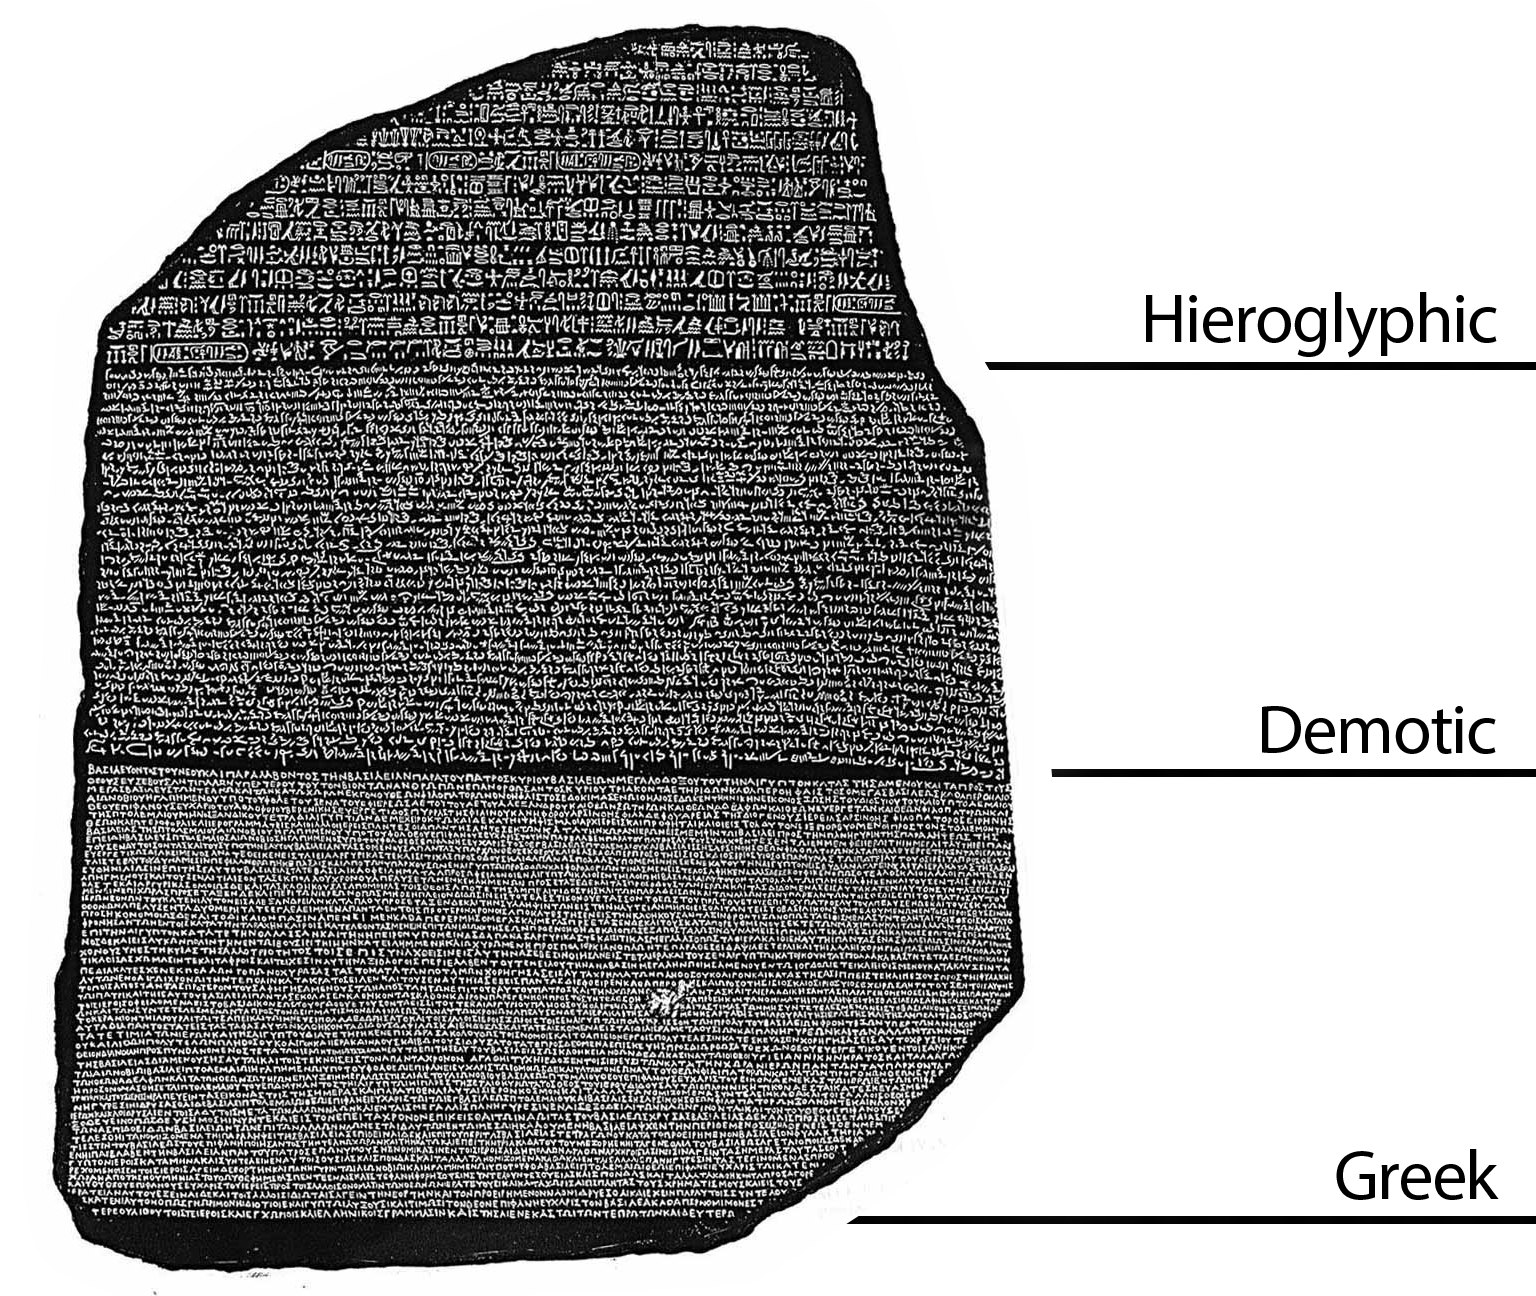
\includegraphics[width=0.6\textwidth]{images/rosetta_stone.png}
\end{figure}

The existence of parallel data is the most important prerequisite for building an effective SMT system. Today there exist a plenty of both monolingual and sentence-aligned parallel data. Such a collection of corpora is for example OPUS~\cite{Tiedemann12}. One of the richest sources of the parallel data included in OPUS are texts produced by government organizations, such as the European Parliament Proceedings, which are being translated into each of the 23 official languages of the European Union. Other important sources we could mention are movie subtitles, books, news websites, or localization files of computer software. 

We believe that the web is a potential source of considerable amounts of parallel data generated not only by well-known organizations like the European Parliament but also by organizations of smaller sizes and by individuals. In the field of SMT there is also motivation and need for acquisition of parallel data from various domains. To illustrate this motivation, an SMT system trained on just the parallel data from the European Parliament Proceedings may seem cumbersome in translation of standard speech language because of the formal nature of the training data. We assume that by mining parallel data from the web, we can obtain useful parallel corpora which would also reflect the natural distribution of domains.

\section*{Goals}

The main goal of our thesis is to propose a method for solving the task called \textit{bilingual document alignment} applicable in the field of mining parallel data from the web. This problem can be generally stated as follows: assume we have a set of documents written in two different languages, where a document is a plain text not limited by length; it can be a sentence, a sequence of multiple sentences, or even a single word. The solution of this task is a collection of all such pairs of documents in different languages that are mutual translations of each other.

We would like to distinguish our method by taking a different approach than the one shared by many others. The majority of methods developed in the field primarily use the structure of the web pages in the alignment process. We believe that by performing structure similarity filtering, we can lose a considerable part of parallel data. 

The aim is to propose a more generic method, not based on page structure comparison. The method is expected to find bitexts located on pages not at all similar in structure. In other words, our motivation is to find the parallel segments, i.e.\ paragraphs we consider as input documents to our method, contained on a given bilingual web domain, regardless of the structure of its web pages. By moving to these finer units, we also have to rely more on the actual content of the paragraphs. To overcome the well-known problems of data sparseness, we plan to use currently popular models like \textit{word2vec}~\cite{Mikolov13a}\cite{Mikolov13b}\cite{Mikolov13c}, and to deal with the possibly large amount of input documents, we intent to make use of recently studied strategies for \textit{locality-sensitive hashing}~\cite{Charikar02}\cite{Andoni08}.

Any finer alignment of the documents, such as sentence alignment, is beyond the scope of our work. The methods for achieving sentence alignment for a document-aligned parallel corpus are well examined~\cite{Tiedemann11} and can be easily applied to the output of our method. 

Moreover, our particular requirements for the target method are scalability and reasonable behavior on noisy and sparse data, where only some of the input documents will have a pair. Both these requirements are needed when processing data from the web. It is also important to mention that the method is expected to be supervised, which means it depends on the provided a priori knowledge in the form of an already existing sentence-aligned bilingual text corpus that is used in the training process. However, this does not mean that the training corpus needs to cover every single word contained in the actual input documents. 

Another goal of this work is to perform experiments with the proposed method and present their results. Our experiments are solely focused on the Czech--English~\cite{Bojar12_1} language pair. The first experiment is carried out using CzEng 1.0~\cite{Bojar12_2}---a Czech--English sentence-aligned parallel corpus. This way we can measure the quality of the results automatically. The second experiment uses more realistic, noisy data provided by the Common Crawl Foundation~\cite{CommonCrawl}---a non-profit organization with the goal of democratizing access to web information. It produces and maintains an open repository of web-crawled data that is universally accessible and analyzable.

\section*{Outline}

The rest of this thesis is organized as follows. Chapter~\ref{chapter:related_work} introduces the related work in this field, covering similar approaches that have been already explored. They can still serve as an inspiration for the potential extension of ideas covered in the thesis. In Chapter~\ref{chapter:background_work_and_prerequisities} we discuss technologies used in our work, together with reasoning and motivation for their selection. Chapter~\ref{chapter:proposed_method} contains a detailed description of the proposed method with all implementation details. Chapter~\ref{chapter:prealigned_data_czeng_experiment} describes the experiment done on the CzEng 1.0 corpus. In Chapter~\ref{chapter:web_data_common_crawl_experiment} the experiment done on the Common Crawl dataset is explained, along with a way how to mine parallel corpora from the vast amounts of real-world web data. The final chapter concludes the discussion and suggests potential directions of future work.
%%%%%%%%%%%%%%%%%%%%%%%%%%%%%%%%%%%%%%%%%%%%%%%%%%%%%%%%%%%%%%%%%%%%%%%%%%%%%%%%
%% MASTER'S THESIS                                                            %%
%%                                                                            %% 
%% Title (en): Mining Parallel Corpora from the Web                           %%
%% Title (sk): Rafinácia paralelných korpusov z webu                          %%
%%                                                                            %%
%% Author: Bc. Jakub Kúdela                                                   %%
%% Supervisor: Doc. RNDr. Irena Holubová, Ph.D.                               %%
%% Consultant: RNDr. Ondřej Bojar, Ph.D.                                      %%
%%                                                                            %%
%% Academic year: 2015/2016                                                   %%
%%%%%%%%%%%%%%%%%%%%%%%%%%%%%%%%%%%%%%%%%%%%%%%%%%%%%%%%%%%%%%%%%%%%%%%%%%%%%%%%

\chapter{Related Work}
\label{chapter:related_work}

This chapter describes methods that are the closest to ours. All approaches mentioned in the following text have one thing in common---their goal is to harvest parallel corpora from the web.

\section{Bitextor}
\label{section:bitextor}

Bitextor\footnote{\url{https://sourceforge.net/projects/bitextor/} (accessed March 20, 2016)}~\cite{EsplaGomis09}\cite{EsplaGomis10} is a well maintained free and open-source bitext generator which obtains its base corpora from the Internet. First, it downloads an entire website, keeping only the files in the plain text, HyperText Markup Language (HTML)~\cite{HTML} or Extensible Markup Language (XML)~\cite{XML} format. Then the system detects the language of each file and applies a group of heuristics to find possible candidate pairs of files which can have the same content. These heuristics include for example file size comparison, HTML tag structure edit distance, and text blocks length difference. Once it has identified the candidate pairs of files, it generates a bitext output in the Translation Memory eXchange (TMX)~\cite{TMX} format. 

Since the first release of Bitextor, the system has evolved and has been extended with features like heuristics based on Uniform Resource Locator (URL) and utilization of dictionaries with the bag-of-words model to help the candidate filtering process. The following text describes the current state of the core pipeline of Bitextor according to the standard workflow.

\subsection{Bitextor: Procedure}
\label{subsection:bitextor_procedure}

\begin{enumerate}
	\item Bitextor downloads all text/HTML/XML files from a website provided by seed URLs, while keeping their folder structure. For this purpose it internally uses a crawler called HTTrack\footnote{\url{http://www.httrack.com/} (accessed March 20, 2016)}.
	
	\item It extracts encoding, MIME type and Base64-encoded content of each downloaded file. The library called boilerpipe\footnote{\url{https://github.com/misja/python-boilerpipe} (accessed March 20, 2016)} helps to remove menus and other unwanted parts from the HTML files. Then the tool Apache-Tika\footnote{\url{http://tika.apache.org/} (accessed March 20, 2016)} is used to repair the structure of the HTML files, obtaining XHTML~\cite{XHTML} files. This step also normalizes encoding of the files into uniform UTF-8.
	
	\item The system identifies the language of the files. This step is done using langid.py\footnote{\url{https://pypi.python.org/pypi/langid} (accessed March 20, 2016)}~\cite{Lui12}, which is a standalone language identification tool pre-trained for a large number of languages.

	\item A so-called \textit{raspa} representation is created for every HTML file. In order to create such a representation every text block is replaced by the sequence of apostrophes, of length $\log_2(\operatorname{len}(\operatorname{text}))$, where $\operatorname{len}(\operatorname{text})$ is the length (in characters) of the given text block. This means that the representation preserves the HTML tags in-place, only the text blocks are changed. These raspa representations will later help the system to calculate the \textit{fuzzy-matching score} used to rank the parallel file candidates.
	
	\item The next step uses the bag-of-words from each file and a provided dictionary to compute an overlapping score between the files in both languages. For each file in one language, it creates a list of ten highest scoring candidates in the other language. The default dictionary contains English, Spanish, Catalan, Croatian, and Basque languages.
	
	However, the system provides a script for creating a custom dictionary. This script gets a sentence-aligned bilingual corpus in the languages we want to consider, lowercases it, and filters out overly long sentences. Then it runs GIZA++\footnote{\url{http://www.statmt.org/moses/giza/GIZA++.html} (accessed March 20, 2016)}, a word-alignment tool that implements the series of IBM Models introduced by Brown et al.~\cite{Brown93}. Bitextor lets GIZA++ dump parameters of the trained statistical models for both directions (one language as the source and the other as the target, and vice versa). Finally, each word pair appearing in both directions and having the value of harmonic mean of parameters great enough is included into the dictionary.
	
	\item With the candidate lists created, the system recalculates the scores provided by the previous step. It multiplies the score of each candidate by the fuzzy-matching score between the raspa representations of the file and the candidate. The fuzzy-matching score compares two raspa sequences on the basis of Levenshtein's edit distance. To calculate the edit distance the system internally uses the python-Levenshtein\footnote{\url{https://pypi.python.org/pypi/python-Levenshtein/} (accessed March 20, 2016)} library.
	
	\item Bitextor allows to create the candidate lists in both directions (one language as the source and the other as the target, and vice versa). In this situation, the score for a file pair is calculated as an average of scores for both directions. If the file pair scores below the threshold in either of the directions it is discarded altogether.
	
	\item All aligned files are first concatenated and stored in two new files, one for each language. Concatenation is done in the same order, while using a system-specific separator. The presence of separators ensures that segment alignment will happen only between the aligned files. Then the system runs hunalign\footnote{\url{http://mokk.bme.hu/resources/hunalign/} (accessed March 20, 2016)}~\cite{Varga05} to get the segment alignment. In the first pass, it uses Gale-Church~\cite{Gale93} sentence-length algorithm for the alignment. Next, it creates an automatic dictionary from the first alignment. Then it realigns the text in the second pass, using the automatic dictionary.
	
	\item After running hunalign, the system removes all unaligned segments and those with a confidence score below a specified threshold. Moreover, the system allows a configuration in which the aligned pairs of segments coming from a pair of files with too many problems are discarded. Finally, with the segments aligned and filtered, Bitextor can, optionally, output them in the TMX format.
\end{enumerate}

\subsection{Bitextor: Results}
\label{subsection:bitextor_results}

The system's authors suggest favoring precision over recall. They performed an experiment covering two websites. The system's output was compared against human evaluations. The preliminary results show a great precision of approximately $100\%$ at a reasonable recall of more than $63\%$.

\subsection{Bitextor: Summary}
\label{subsection:bitextor_summary}

We consider Bitextor as a mature, language independent tool which can handle many typical scenarios when facing the problem of harvesting parallel corpora from multilingual websites. Yet its functionality is based on a premise that parallel texts are stored in files with very similar HTML structure. However, there are many websites which are designed in such way that all the information is available in the primary language, with only a subset translated into secondary languages. As an example, consider a news website where each article is written in the primary language, starting with a summary followed with a body. But each of these articles has a translation available only for the summary part. This means that the page with the article written in the primary language has a different HTML structure than the page containing just the translated summary. They probably differ in the number of paragraph tags, and thus Bitextor would discard such pair due to the difference in both HTML structure and text length. Also, in the case where a single page contains a same piece of text available in both the languages, Bitextor would not find such bitext.

\section{PaCo\textsuperscript{2}}
\label{section:paco2}

PaCo\textsuperscript{2}~\cite{Vincente12} is a fully automated tool for gathering parallel corpora from the web. Unlike others, it is also focused on identification of potential websites containing bilingual content for chosen languages. Being language independent, it is adaptable to any set of languages. The architecture of PaCo\textsuperscript{2} is designed as a pipeline consisting of three main phases. In the first, phase the web is searched for websites which might contain bilingual textual content. In the second phase, parallel web pages are detected on the sites identified in the previous phase. In the third and final phase, parallel web pages are aligned at the sentence level and a parallel corpus is created. The details of each phase are described in the list below.

\subsection{PaCo\textsuperscript{2}: Procedure}
\label{subsection:paco2_procedure}

\begin{enumerate}
	\item PaCo\textsuperscript{2} handles bilingual website detection. This custom capability is a relatively unique feature in the field. It has also been implemented in the previous approaches (e.g. STRAND); however, they were entirely dependent on the AltaVista search engine, which had an application programming interface (API) that allowed to search for multilingual websites. Unfortunately, it is no longer available. 
	
	The system uses search engines for identification of potential bilingual websites. As an input, it requires a language pair and a list of fifty or more lemmatized words from the preferably less frequent of the two languages. It then generates queries for the search engine. The queries are triplets from the list of provided words. When querying the search engine, the system uses its API to request the results for the other language. This way, a list containing URLs of candidate websites is created. 
	
	\item The preliminary filter is applied to discard a priori unwanted candidates, such as gigantic websites, blog platforms, and social media. Authors have found out that these would bring a very negligible benefit. For each of the URLs left in the filtered list, the system downloads a very small part of the website and searches for elements of parallelism, e.g. hyperlinks with anchor texts or \texttt{alt} attribute texts indicating presence of languages. If the website passes the set of requirements on this smaller scale it is considered as a website with parallel content.
	
	\item For each website found in the previous step, the system harvests all of its HTML files using Wget\footnote{\url{https://www.gnu.org/software/wget/} (accessed March 27, 2016)}. In order to compare each pair of the $N$ acquired files, the system would need to perform $N^2$ comparisons in the worst case. However, various heuristics and statistical filters are applied to reduce this number. These include language, file size, and length comparison. The system compares only HTML files written in the exact two languages requested by the user. It also excludes all file pairs outside a certain similarity threshold with regard to the file size and length ratio. Language identification is performed using TextCat\footnote{\url{http://www.let.rug.nl/vannoord/TextCat/} (accessed March 27, 2016)}, and character encoding is standardized to UTF-8 by means of BeautyfulSoup\footnote{\url{http://www.crummy.com/software/BeautifulSoup/} (accessed March 27, 2016)}. 
	
	Authors of PaCo\textsuperscript{2} decided to keep boilerplate\footnote{surplus ``clutter'' (templates) around the main textual content of a web page} parts because they consider the menus and other elements such as breadcrumbs to contain useful parallel information. In addition, each content having the same value regardless the language of the text (e.g. copyright notes or contact information) is removed from the results. The bitext detection module runs the following three major filters when searching for parallel files:
	
	\begin{enumerate}
		\item \textit{Link Follower Filter} focuses on the hyperlinks located in HTML structures of the files. For example, let us assume we want to find parallel HTML files for the language pair consisting of Czech and English. If there exists an HTML file pair where the structure of the first file contains a hyperlink to the second file and vice versa, and additionally, if the links contain reasonable anchor texts like ``English'', ``anglicky'' and ``Czech'', ``česky'', the filter considers the pair of files as parallel.
		
		\item \textit{URL Pattern Search} draws from the assumption that parallel web pages have usually similar URLs. They often differ only in parts representing language codes. For instance, the following two URLs referencing parallel files differ only in this manner. Czech article contains ``cs'' in its URL, while the English one contains ``en'' instead.
		
		\vspace{1em}
		\footnotesize
		\texttt{http://www.mff.cuni.cz/to.cs/verejnost/konalo-se/2016-03-cenaprop/}\newline
		\texttt{http://www.mff.cuni.cz/to.en/verejnost/konalo-se/2016-03-cenaprop/}
		\normalsize
		\vspace{1em}
		
		To detect such scenarios, for each pair of file, PaCo\textsuperscript{2} first finds and removes the language codes from both URLs. Then it calculates the Longest Common Subsequence Ratio (LCSR). If the ratio reaches a required threshold the system considers the candidates as parallel files.
		
		\item \textit{HTML Structure and Content Filter} is useful in all other scenarios not covered by the previous two filters. The system compares HTML tag structure information~\cite{Resnik03} combined with content similarity. PaCo\textsuperscript{2} authors observed that by comparing only the HTML structures of the files the results are poor due to the existence of numerous files with similar HTML structures on an ordinary website. 
		
		In order to compare content similarity, the system works with extracted universal entities, e.g. numbers, email addresses and dates. The algorithm for extraction of these language independent entities  has been adapted from the previous work in the field~\cite{Nadeau04}. To compute the content similarity of candidate parallel files, vector representation consisting of extracted entities is prepared for each file. The order of entities corresponds to the order of their appearance in the content. The Ratcliff/Obershelp~\cite{Ratcliff88} pattern recognition algorithm is then used to compare these vectors.
		
		To calculate the total score for a given pair of candidate parallel files, their HTML structure similarity and content similarity is calculated. Both results are weighed, and those candidates that reach a certain threshold are regarded as parallel files. If there are multiple candidates that have reached the threshold to be a parallel file with one file, all of them are ruled out.
	\end{enumerate}
	
	\item Sentence alignment is done with the help of the hunalign tool. Then, a series of post processing activities is applied. Translation units (i.e.\ pairs of sentences) are sorted and deduplicated. Units containing solely elements like numbers, email addresses, or URLs are excluded. Language identification is done once again, but this time at the sentence level. Units that do not fit the requested languages are discarded. At the end of the process, if there are more than two unique target texts for the same source text, all units containing this source text are omitted in favor of precision. The output can be either in raw text or in the TMX format.
\end{enumerate}

\subsection{PaCo\textsuperscript{2}: Results}
\label{subsection:paco2_results}

PaCo\textsuperscript{2} authors report experiments on these language pairs: Basque--Spanish, Spanish--English and Portuguese--English. In order to identify the bilingual websites, PaCo\textsuperscript{2} utilized the Bing\footnote{\url{http://www.let.rug.nl/vannoord/TextCat/} (accessed March 27, 2016)} search engine. Results show acceptable precision of $97\%$ for the Basque--Spanish language pair. However, the precision levels for the Spanish--English and Portuguese--English pairs were relatively poor, $67\%$ and $78\%$ respectively. Error analysis over the wrong candidates showed the accuracy of the system to be low due to the fact that many of the web pages covered in the experiment contained dynamically variable elements (e.g. tag-clouds).

\subsection{PaCo\textsuperscript{2}: Summary}
\label{subsection:paco2_summary}

PaCo\textsuperscript{2} is a language independent system. Its unique feature of identification of websites containing parallel data is beneficial. The aligning process is entirely unsupervised, which we also consider a valuable feature. The only a priori knowledge required to run the whole process of parallel data acquisition is a list of fifty or more lemmatized words from one of the two chosen languages. We appreciate the focus on performance, where PaCo\textsuperscript{2} uses a set of heuristics. These identify and handle common scenarios, which leads to faster delivery of results. Unfortunately, like Bitextor, PaCo\textsuperscript{2} cannot handle alignment of parallel data segments located in files with different HTML structure. 

\section{STRAND}
\label{section:strand}

STRAND~\cite{Resnik03}\cite{Resnik99}\cite{Resnik98} is a system performing structural translation recognition. Its main objective is to identify pairs of parallel web pages. Its design is based on an observation of how parallel content is usually distributed over an ordinary website. The authors suggest that websites have a very strong tendency to present parallel content via pages having a similar HTML structure. The text below describes how the system works.

\subsection{STRAND: Procedure}
\label{subsection:strand_procedure}

\begin{enumerate}
	\item At the beginning of the process, STRAND tries to locate websites containing parallel data. For this task, it used to utilize advanced search capabilities of the AltaVista search engine which, unfortunately, is no longer active. The engine helped with searching for two types of web pages:

	\begin{itemize}
		\item A \textit{parent} page contains hyperlinks to web pages containing different language versions of the same content. An example of such a page is one containing two links to the same article written in English and French. To perform search for such a page, the system queries the engine with an expression \texttt{(anchor:"english" OR anchor:"anglais") AND (anchor:"french" OR anchor:"français")}. Additionally, a distance filter is applied on the obtained results. If the positional distance between the links within the HTML structure is more than $10$ lines, the page is filtered out. Authors believe that parent pages tend to have links pointing to the corresponding pages closely located within their HTML structures.
		
		\item A \textit{sibling} page is a type of page in one language that contains a hyperlink to a version of the same page in another language. A page written in French containing an anchor with a label "English", which points to another page with the same content in English, is an example of a sibling page. The system searches for these by querying the engine with an expression like \texttt{(anchor:"english" OR anchor:"anglais")}.
	\end{itemize}
	
	After AltaVista search engine was shut down, authors added another component to the system called \textit{spider}. It can download all the web pages from a provided initial list of websites.
	
	\item Generating candidate pairs is simple when a search engine is used to acquire the list of parent and sibling pages. For each parent page, the system takes the two linked pages, and for each sibling page, the system takes the page together with the linked one. 
	
	However, when all the pages from a website are under consideration, naturally, the task of generating candidate pairs is more difficult. The spider component contains a URL-matching stage which exploits the fact that parallel pages have usually similar URL structure. The system knows substitution rules which help to detect if a URL of a page in one language can be transformed into a URL of another page in a different language. If so, these two pages are considered as a candidate pair. Web pages that are mutual translations tend to have a very similar ratio of lengths; therefore, the system requires from a candidate pair to have a reasonable value of this ratio, otherwise it is discarded.
	
	\item The key element of STRAND is a structural filter. It analyses HTML structure of both pages of a candidate pair and decides whether they are parallel or not. First, the system linearizes the HTML structure while ignoring the textual content of the page. As a result, it generates a linear sequence of tokens for each HTML structure. Such a sequence consist of three types of tokens:

	\vbox{
	\begin{itemize}
		\item \texttt{[START:element\_label]};
		\item \texttt{[END:element\_label]};
		\item \texttt{[Chunk:text\_length]}.
	\end{itemize}
	}
	
	First two types of tokens are substitutes for HTML opening and closing elements. The last type of token is a substitute for a non-markup text block. The length is calculated as the number of non-whitespace bytes contained within the block. The attributes of the HTML elements are treated similarly as a non-markup block. For example \texttt{<font color="blue">} would generate a subsequence \texttt{[START:font][Chunk:12]}. These sequences, representing linearized structure of both web pages, are aligned by means of an adapted algorithm~\cite{Hunt75} based on dynamic programming. With alignment done, the system calculates 4 scalar values, which eventually determine whether the candidate pair is parallel or not. These values characterize the quality of the alignment, but also the probability of the candidate pair to be parallel:
		
	\begin{itemize}
		\item \textit{dp} \quad The difference percentage of the non-shared tokens. It represents the ratio of mismatches in the alignment. Mismatches are tokens from one sequence not having a corresponding token in the other sequence and vice versa. The greater ratio indicates that the two web pages have different structure and therefore are less likely parallel. This can also happen when the one page contains the full article while the other contains only the translation of its introduction. The system requires the value to be less than $20\%$.
		
		\item \textit{n} \quad The number of aligned non-markup text blocks of unequal length. The aligning algorithm maximizes the number of matches of the identical tokens which represent markup. As a side effect, it also pairs the tokens of the corresponding non-markup text blocks. The higher number of aligned pairs of the non-markup text blocks is found, the more likely it is the web pages are parallel.
		
		\item \textit{r} \quad The correlation of lengths of the aligned non-markup blocks. The authors assume that for each pair of parallel web pages, it is likely that the lengths of their corresponding text blocks are in linear relationship. This means that shorter text blocks of one page correspond to the shorter text blocks of the other page, and so it is with medium and longer blocks. The Pearson~\cite{Pearson95} correlation coefficient is approximately $1.0$ in such scenarios, indicating positive correlation.
		 
		\item \textit{p} \quad The significance level for the correlation of lengths of the aligned non-markup blocks. This measure describes the reliability of the previous one. The system requires the value to be less than $0.05$, which corresponds to more than $95\%$ confidence that the correlation value was not obtained by chance.
	\end{itemize}
\end{enumerate}

\subsection{STRAND: Results}
\label{subsection:strand_results}

At first, the authors used a set of manually, empirically chosen thresholds for the discussed scalar values based on their observations from an experiment with English--Spanish development data. The thresholds seemed to perform well also when testing on English--French and English--Chinese data. Later, they investigated options of optimizing the binary decision task, whether to label the candidate pair of web pages as parallel or not, based on the mentioned scalar values. They came up with the idea of building a supervised classifier utilizing the C5.0\footnote{\url{http://www.rulequest.com/demoeula.html} (accessed April 3, 2016)} decision tree software. With the original manually chosen thresholds, the system achieved $68.6\%$ recall at $100.0\%$ precision, while using the learned classifier it achieved $84.1\%$ recall on average at the cost of lower $95.8\%$ precision.

\subsection{STRAND: Summary}
\label{subsection:strand_summary}
	
STRAND is one of the pioneers in the field of tools for parallel corpora acquisition from the web. Its authors have introduced some of the ideas still present in other similar tools. We consider the later added supervised binary classification as an effective approach.

\section{Mining Wikipedia}
\label{section:mining_wikipedia}

In previous related work, the researchers have developed a method~\cite{Wolk14} that can build subject-aligned comparable corpora, which are later refined to obtain truly parallel sentence pairs. The efficiency of the method is demonstrated on the Polish--English Wikipedia\footnote{\url{https://www.wikipedia.org/} (accessed April 3, 2016)} content. 

In order to better understand this method, the authors suggest distinguishing between a few types of corpora according to their properties:

\begin{itemize}
	\item A \textit{parallel corpus} is the most valued and rare type. It can be defined as a corpus that contains quality translations of documents in multiple languages. Such a corpus is already aligned or should be very easy to align at the sentence level.

	\item A \textit{noisy-parallel corpus} contains bilingual sentences that are not perfectly aligned or the quality of the translations is poor. However, the majority of documents should be present in the corpus, including their translations.
	
	\item A \textit{comparable corpus} consists of bilingual documents that are neither sentence-aligned nor mutual translations. Nevertheless, the documents should be at least topic-aligned.
	
	\item A \textit{quasi-comparable corpus} includes very heterogeneous and very non-parallel documents that do not even have to be topic-aligned. 
\end{itemize}

The authors have proposed a methodology which can extract a truly parallel corpus from a non-sentence-aligned one, such as a noisy-parallel or comparable. The implementation of the methodology has the form of a pipeline which includes specialized tools for obtaining, aligning, extracting, and filtering text data. This pipeline is explained in the following text.

\subsection{Mining Wikipedia: Procedure}
\label{subsection:mining_wikipedia_procedure}

\begin{enumerate}
	\item Web crawling is the first step in the process. The pipeline includes a specialized web crawler dedicated solely to processing the Wikipedia website. The crawler requires a hyperlink to a specific article, preferably written in the less frequent of the two languages. For the Polish--English language pair this would be Polish. With the link to the Polish article, the crawler downloads its page and also other pages in the topic domain (following the links on the pages), together with their corresponding English versions. With the HTML web pages obtained, the crawler extracts and cleans their textual content. This means that all links, figures, pictures, menus, references, and other unwanted parts of the data are removed from further processing. The bilingual extracted texts are then tagged with unique IDs to form a topic-aligned comparable corpus.
	
	\item The system uses a two-step sentence alignment method provided by hunalign. The pipeline does not provide any dictionary to hunalign. Without a dictionary, hunalign first aligns the sentences using just the Gale-Church~\cite{Gale93} sentence-length algorithm. Then it builds an automatic dictionary based on the sentence alignment from the first run. This dictionary is used in the second run to realign the alignment, improving the result.
	
	Like the majority of sentence aligners, hunalign does not perform well when the order of corresponding segments is different for two languages. This happens when segment ``A'' is followed by ``B'' in one language, while in the other one ``B'' is followed by ``A''. The method deals with this problem by applying a posteriori filtering process on the results obtained from the hunalign. The goal of the filtering process is to find the correct alignment for each source sentence if such alignment exists, or to remove the sentence from the resulting corpus otherwise.
	
	\item The filtering strategy of the pipeline is to find the correct translation for each Polish sentence using a translation engine. Given an MT system, the filtering process first translates all the Polish sentences into English. Then it uses a series of heuristics to compare the obtained machine-translated sentences with the original English sentences. The authors have considered many ways to measure the similarity of two sentences in the same language. 
	
	One of the measures is defined as the number of common words divided by the total number of words in both sentences. Removing the stop words\footnote{usually the most common words in the language with very little meaning} (e.g. ``a'' or ``the'') prior to the measurement yields more precise results. When comparing the machine translated sentence with the original one, the translated one often contains a stem of a corresponding word (e.g. ``boy'' vs ``boys''). This cannot be detected by the described measure. Another important aspect ignored by this measure is the order of words. To tackle this, the authors added another measure based on the concept of string similarity.

	Synonyms are another problem. In order to take them into account the method uses WordNet\textregistered{}\footnote{\url{https://wordnet.princeton.edu/} (accessed April 3, 2016)}~\cite{Miller95}\cite{Fellbaum98} together with the NLTK\footnote{\url{http://www.nltk.org/} (accessed April 3, 2016)}~\cite{Loper02} Python module. The method generates multiple derived sentences for each original sentence using synonyms. The generated sentences are then compared in a many-to-many relation.
	
	To obtain the best results, the script that covers the filtering process provides the ability to let the user choose multiple filtering heuristic functions with different acceptance rates. The faster functions, usually with lower quality results, are calculated first. If they find a result with a very high acceptance rate, their result is accepted as the final one. Otherwise, slower functions, with higher precision in general, are used in the filtering process.
\end{enumerate}

The filtering procedure of the method requires a translation engine. A custom one was built to be used. The training data included Polish--English parallel data for various domains from OPUS. To increase the system's precision, the authors adapted it to Wikipedia using the dump of all English content as a language model. The underlying MT system was based on Moses~\cite{Koehn07}\cite{Moses} toolkit.

\subsection{Mining Wikipedia: Results}
\label{subsection:mining_wikipedia_results}

The conducted experiments show that the filtering method has quite good precision of more than $95\%$. The results also correlate with human evaluations. The method is language independent and supervised, as it needs a parallel corpus for the initial training of the SMT system. The amount of obtained data, in other words, the method's recall, is absolutely not satisfactory. Authors suggested that an iterative approach could increase the recall. In such a scenario, after each iteration, the newly acquired parallel corpus would help to build a domain-specific vocabulary for hunalign and to retrain the SMT system.

\subsection{Mining Wikipedia: Summary}
\label{subsection:mining_wikipedia_summary}

The described pipeline shares some common features with our method. In particular, both methods focus on extraction of truly parallel corpora from noisy data. Unfortunately, it is hard to tell to what extent it would be possible to optimize the set of chosen heuristic functions and their acceptance rates to gain better overall recall. This would require further experiments with the system, which would need to be obtained and deployed locally.

\section{Mining Common Crawl}
\label{section:mining_common_crawl}

Another interesting project~\cite{Smith13} closely related to ours is the one focused on mining parallel corpora on the web-scale from the Common Crawl~\cite{CommonCrawl} dataset. This work is heavily based on the previously described and discussed STRAND~\cite{Resnik03} algorithm. Using a set of common two- or three-letter language codes, this method achieved to mine parallel corpora for dozens of language pairs from 32 terabyte (TB) large dataset in a time span shorter than a single day. The amount of parallel data acquired in this way is large and the quality is reasonable. Moreover, the parallel corpora obtained cover data from various domains. These corpora provably increase the performance of machine translation systems if included in the training process.

The authors argue that any sophisticated method for mining parallel corpora from the web requires direct access to a larger dataset consisting of crawled web pages together with the computing power to process them. They claim that these large-scale web-crawled datasets were, until recently, available solely to large companies with the resources to crawl, store, and process the data from the entire web. Only recently, the Common Crawl non-profit organization began to provide a large-scale partial copy of the web to researches, companies, and individuals at no cost for research and analysis.

The Common Crawl corpus is stored and hosted by Amazon Web Services\footnote{\url{https://aws.amazon.com/} (accessed April 4, 2016)} as a part of Public Data Sets\footnote{\url{https://aws.amazon.com/public-data-sets/} (accessed April 4, 2016)} in Simple Storage Service (S3)\footnote{\url{https://aws.amazon.com/s3/} (accessed April 4, 2016)}. It can be either downloaded to a local cluster, accessed from Amazon Elastic Compute Cloud (EC2)\footnote{\url{https://aws.amazon.com/ec2/} (accessed April 4, 2016)}, or processed using the Amazon Elastic MapReduce (EMR)\footnote{\url{https://aws.amazon.com/elasticmapreduce/} (accessed April 4, 2016)} service. This section includes only a brief description of the Common Crawl dataset and the MapReduce~\cite{Dean04} framework necessary for us to understand this project. The following text describes the flow of the method proposed by this project.

\subsection{Mining Common Crawl: Procedure}
\label{subsection:mining_common_crawl_procedure}

\begin{enumerate}
	\item The first step in the pipeline performs identification of potentially parallel pairs of web pages, using the Amazon EMR framework. This is the only step executed remotely on the Amazon servers. All the other steps are performed locally, using the downloaded dataset created in the first step. The Amazon EMR is chosen as the processing framework because the MapReduce paradigm suits the task well. For the sake of brevity, we can describe the Common Crawl corpus as a huge set of crawled and stored web pages in the form of HTML requests and their responses. To briefly introduce the MapReduce framework, it is a mechanism which allows us to iteratively process all the crawled HTML requests and responses in the corpus in a distributed manner. 
	
	The method starts by remotely executing the MapReduce application, which implements two phases: \textit{map} and \textit{reduce}. The intention is to scale down the vast amount of crawled web pages to a selection of candidates possible to process locally.
	
	During the map phase, the method iterates over each web page entry in the corpus. It scans the URL of the page, searching for the occurrences of two types of substrings:
	
	\vbox{
	\begin{itemize}
		\item Language codes in ISO 639 format (two- or three-letter codes).
		\item Language names in English and also in the language of their origin.
	\end{itemize}
	}
	
	If such a substring, surrounded by non-alphanumeric characters, is present in the URL the page is identified as potentially having parallel versions. In this case, the method outputs the URL of the page with the matching substring replaced by a single asterix symbol. It also marks down the language associated with the replaced substring. For example, when processing the page with URL \texttt{http://www.ksi.mff.cuni.cz/en/}, the method would output the following key-value pair with the composite value:
	
	\vbox{
	\begin{itemize}
		\item Key: \texttt{http://www.ksi.mff.cuni.cz/*/}.
		\item Value:
		\begin{itemize}[label=$\circ$]
			\item \texttt{http://www.ksi.mff.cuni.cz/en/} (original URL);
			\item English (language associated with the code);
			\item full HTML structure of the web page.
		\end{itemize}
	\end{itemize}
	}
	
	In the reduce phase, the method obtains all the values having the same key, i.e the  language-independent URL. If there are at least two items associated with the same key having different languages marked down, the method outputs all the values for such a key.
	
	Upon completion of the MapReduce execution, the resulting dataset is downloaded to a local cluster for further processing. This dataset is relatively small compared to the original one, and it can be processed locally.
	
	\item The rest of the process is similar to STRAND (see Section\ref{section:strand}). In order to determine which web pages are parallel, the method linearizes their HTML structures in the same way as STRAND does. Additionally some HTML elements are ignored (e.g. \texttt{<font>} or \texttt{<a>}). The pairs of sequences are aligned using an algorithm based on dynamic programming which optimizes the number of matching tokens. The alignment is used to calculate the same set of measures defined by STRAND. The result of this step is a set of matching text blocks gathered from the pairs of corresponding web pages.
	
	Also inspired by STRAND, the project's authors tried to train the maximum entropy classifier for the Spanish--English language pair by using a set of 101 manually aligned and annotated pairs of web pages. However, it turned out that even when using the best performing subset of the features, the classifier did not outperform a na\"{\i}ve one, which considers every pair of web pages to be parallel. They argue that this was caused by the unbalanced nature of the annotated training data, where $80\%$ of the pairs were parallel. In the end, they decided to exclude the classifier from the pipeline.	
	
	\item The pairs of matching text blocks then pass through the process of segmentation. The method uses the Punkt sentence splitter from the NLTK~\cite{Loper02} Python module to perform segmentation at both the sentence and word level.
	
	\item With segmentation done, each of the matching text blocks is sentence-aligned using the Gale and Church~\cite{Gale93} algorithm. The output of the execution can be regarded as a parallel corpus.
	
	\item Lastly, the process includes the final cleaning of the produced parallel corpus. The whole pipeline does not perform any boilerplate removal in the previous steps. Since the authors decided not to do so, they at least proposed to remove the pairs of segments where either both segments are identical, or one of the segments appears multiple times in the corpus.
\end{enumerate}

\subsection{Mining Common Crawl: Results}
\label{subsection:mining_common_crawl_results}

To estimate the recall of the heuristic used for candidate selection, the same method was applied on a set of previously mined parallel pairs of URLs included in the French--English Gigaword~\cite{Burch11} corpus. As a result, $45\%$ of all pairs have been discovered. Inclusion of one-letter language codes (e.g. ``f'' for French, ``e'' for English) increased the recall of the method's recall to $74\%$, but the authors decided not to use such codes out of concern that the system might lose precision. In order to estimate the method's precision, a manual analysis was conducted, where 200 randomly selected sentence pairs were compared for 3 language pairs. For the German--English pair, $78\%$ of the mined data represented perfect translations, $4\%$ were paraphrases, and $18\%$ represented misalignments. Additionally, $22\%$ of true positives were probably machine translations, and in $13\%$ of all true positives, one sentence contained some extra content not present in the other.

\subsection{Mining Common Crawl: Summary}
\label{subsection:mining_common_crawl_summary}

In terms of large-scale processing, the project of mining Common Crawl dataset is unique in the field. A special approach is needed when processing hundreds of terabytes large datasets. The Common Crawl dataset is a perfect example of Big Data~\cite{Holubova15}, which are rising in popularity recently. The method is a baseline idea of how to mine parallel corpora from vast amount of web-crawled data.

\section{Summary}
\label{section:related_work_summary}

Bitextor searches for the pairs of parallel web pages by comparing their HTML structures and contents. The structures are compared using a method based on dynamic programming. When comparing the contents, Bitextor uses bag-of-words model powered by a bilingual dictionary. 

PaCo\textsuperscript{2} reduces the number of comparisons by using a set of heuristics including length and file size comparison. To find pairs of parallel web pages, it applies a set of filters. These include inspecting the links between a pair's pages and similarities in their URLs. However, the most important filter compares the HTML structures and contents. Unlike Bitextor, PaCo\textsuperscript{2} compares the contents by identifying the common universal entities (e.g. numbers or e-mail addresses). This approach is unsupervised and language independent.

To reduce the number of comparisons, STRAND uses heuristics similar to those in PaCo\textsuperscript{2}. It comes with an idea to train a decision tree model to classify pairs of web pages as parallel or not. The model uses a set of measures defined on the differences between the two HTML structures. This approach is supervised, as it needs to be trained using a set of, preferably, manually aligned web pages.

The method of mining parallel data from Common Crawl dataset uses the MapReduce framework to refine the candidates, which are then processed locally by a STRAND-like method. The web pages are considered to be candidates if they have the same URLs stripped from the language codes.

The method of mining Wikipedia takes a different approach. For a particular topic, it collects pairs consisting of an article and its version in the other language. The method assumes that the two articles may have different HTML structure and order of the textual context. The pair's articles are aligned at the sentence level, and the resulting alignments are refined with the help of a pre-trained SMT system.

All of the described methods, except the one for mining Wikipedia, search for parallel content only in the form of complete web pages with a similar HTML structure. Although the method for mining Wikipedia does not require the pairs of article pages to have similar structure, the quality of its results depends on the degree of correspondence between the articles' segments and their order.

%%%%%%%%%%%%%%%%%%%%%%%%%%%%%%%%%%%%%%%%%%%%%%%%%%%%%%%%%%%%%%%%%%%%%%%%%%%%%%%%
%% MASTER'S THESIS                                                            %%
%%                                                                            %% 
%% Title (en): Mining Parallel Corpora from the Web                           %%
%% Title (sk): Rafinácia paralelných korpusov z webu                          %%
%%                                                                            %%
%% Author: Bc. Jakub Kúdela                                                   %%
%% Supervisor: Doc. RNDr. Irena Holubová, Ph.D.                               %%
%% Consultant: RNDr. Ondřej Bojar, Ph.D.                                      %%
%%                                                                            %%
%% Academic year: 2015/2016                                                   %%
%%%%%%%%%%%%%%%%%%%%%%%%%%%%%%%%%%%%%%%%%%%%%%%%%%%%%%%%%%%%%%%%%%%%%%%%%%%%%%%%

\chapter{Background Work and Prerequisities}
\label{chapter:background_work_and_prerequisities}

This chapter is an introduction to the resources and tools used in our work. It describes their features and properties and discusses their usefulness in our method or experiments. Before we introduce these individual resources and tools, let us first provide the context in which they are used by outlining the idea behind our method.

\section{Overview of Proposed Method}
\label{section:overview_of_proposed_method}

All the methods described in Chapter~\ref{chapter:related_work} operate on common basic principles. They assume the parallel data are most often created in the form of complete web pages with a similar HTML structure or matching URL, and they work well under these circumstances. However, we believe that there still exists a non-negligible amount of parallel data spread across the web pages that have different HTML structure and URL. Also, the order of corresponding segments may vary in different language versions of the same page. Moreover, some parallel content can be a part of a single web page. We would like to address all these situations.

The majority of described methods start the process by identifying candidate pairs of parallel web pages to be inspected. If a candidate pair has a similar HTML structure then the segments of the two web pages are aligned according to the structure. 

In contrast to these methods, our approach is more generic. The method considers as the input a set of plain text documents for both the languages. These can be all the paragraphs from a bilingual web domain. The intention is to identify candidate pairs of parallel documents. The problem is that for a given web domain, the number of possible pairs of paragraphs is usually significantly greater than the number of possible pairs of web pages. We have to reduce the number of candidate pairs of documents to be inspected as much as possible. Our method is supervised, and in order to be trained, it requires a sentence-aligned training parallel corpus for the given language pair. It begins by learning distributed word representations, i.e.\ word vectors, for both languages using the training corpus. These word vectors are similar for context-related words, even cross-lingually. They are used to calculate aggregate document vectors. Two parallel documents have a similar document vector. The document vectors for one language are subsequently hashed, forming a search index in such a way that similar vectors end up close to each other. The search index is then queried to obtain a short list of candidates for each document in the other language. At this stage, the complexity of the problem is significantly reduced. The method inspects the candidates to determine the best one using a bilingual dictionary. The bilingual dictionary is pre-calculated statistically using the training parallel corpus. This corpus is also used to train the binary classifier, that decides, at the end of the process, whether the pair consisting of a document and its top candidate should be considered parallel or not.

With the basic idea behind the method explained, let us describe the set of resources and tools we use in our work. The details of our method are elaborated in the next chapter.

\section{CzEng 1.0}
\label{section:czeng}

CzEng 1.0~\cite{Bojar12_2} is the fourth release of a sentence-aligned Czech--English parallel corpus, freely available for non-commercial research purposes. It consists of approximately 15 million sentence pairs (233 million English and 206 million Czech tokens) from seven different types of sources. The proportion of these source domains is summarized in Table~\ref{table:czeng}.

To download CzEng 1.0, one must first apply for the registration\footnote{\url{http://ufal.mff.cuni.cz/czeng} (accessed April 5, 2016)}. The corpus can be downloaded in multiple formats. In our experiments, we use all training sections (packs 00--97) of CzEng 1.0 in the plain text, untokenized format. A file in this format contains tab-separated values, where every line stands for a different sentence pair and individual columns represent:

\begin{enumerate}[itemsep=0pt]
	\item Sentence pair ID;
	\item Filter score (indicating the quality of the sentence pair);
	\item Czech sentence (untokenized);
	\item English sentence (untokenized).
\end{enumerate}

Because our method is supervised, it needs a sentence-aligned parallel corpus in order to be trained. For this purpose, we use CzEng 1.0 in our experiments. In one of them, we also utilize the alignment of the corpus to perform the evaluation of the method's efficiency. It is important to note that when using CzEng 1.0 as both the training and testing dataset, we first split the data into two equally sized parts: \textit{head} and \textit{tail}. The head is used for training, while the tail is used for evaluation. The domains are not grouped together within the corpus, but they are shuffled. This means that both head and tail should contain data from each domain.

\begin{table}[!htb]
	\centering
	\caption{CzEng 1.0 source domains distribution (Source:~\cite{Bojar12_2})}
	\label{table:czeng}
	\vspace{1em}
	\begin{tabular}{|l|r|r|}
		\hline
		\textbf{Source Domain} & \textbf{Sentences} & \textbf{Ratio (\%)} \\
		\hline
		Fiction & 4,335,183 & 28.64 \\
		EU Legislation & 3,992,551 & 26.38 \\
		Movie Subtitles & 3,076,887 & 20.33 \\
		Parallel Web Pages & 1,883,804 & 12.45 \\
		Technical Documentation & 1,613,297 & 10.66 \\
		News & 201,103 & 1.33 \\
		Project Navajo & 33,301 & 0.22 \\
		\hline
		\textbf{Total} & 15,136,126 & 100.00 \\
		\hline
	\end{tabular}
\end{table}

\section{MorphoDiTa}
\label{section:morphodita}

MorphoDiTa~\cite{Strakova14}\cite{Spoustova09} (Morphological Dictionary and Tagger) is an open-source tool performing morphological analysis of natural language texts. Its features include morphological analysis, morphological generation, tagging, and tokenization. It can be used either as a standalone tool or a library. 

In our experiment, we want to determine whether lemmatization helps our method get better quality results. For these purposes, we use MorpohoDiTa. As our experiments cover only the texts from the Czech--English language pair, we use available MorphoDiTa models for both Czech~\cite{Straka13} and English~\cite{Straka14}.

\section{SyMGIZA++}
\label{section:symgiza}

SyMGIZA++~\cite{Junczys10} is a tool for computing symmetric word alignment models. It is an extension of MGIZA++, which in turn is a successor of the historically original program called GIZA++.

GIZA++ is an implementation of the IBM Models 1--5~\cite{Brown93}, the HMM model~\cite{Vogel96}, and the Model 6~\cite{Och03}. Comparison of all these models was already analysed and discussed~\cite{Och03}. In the alignment process, it uses an Expectation–Maximization~\cite{Dempster77} (EM) algorithm. This iterative algorithm consists of two steps that are performed in each iteration. In the first step, called the E-step (expectation step), the previously computed model (or the initial model) is applied to the data and expected counts for individual parameters are computed using the probabilities of this model. The second step, called the M-step (maximization step), then takes these expected counts as a fact and uses them to estimate the probabilities of the next model. Furthermore, prior to the training itself, GIZA++ uses the program called mkcls~\cite{Och99} to create word classes. The notion of these classes helps in the training process.

GIZA++ was designed as a single-threaded application. However, MGIZA++~\cite{Gao08} extends GIZA++ with capabilities to run the alignment process in multiple threads on a single computer. This helps the overall speed of the program and reduces the time needed to accomplish the task.

All the models provided by the original GIZA++ are asymmetric. For a chosen translation direction, they allow words to be mapped in a many-to-one, but not in a one-to-many relationship. It is, therefore, quite common and popular to train models for both translation directions and symmetrize the resulting word alignments to allow more natural relationships between words. In this scenario, models for both directions are trained independently and post-symmetrization is applied as the final step of the process. However, the authors of SyMGIZA++ argue that introducing continuous symmetrization, during the whole training process, results in a better quality alignment. Unlike its predecessors, SyMGIZA++ produces results of the symmetrized models. Moreover, it allows us to update these symmetrized models between each iteration of the original training algorithms. The general training scheme,  depicted in Figure~\ref{figure:symgiza}, illustrates all the moments when the model parameters are combined during the process.

\begin{figure}[!htb]
	\centering
	\caption{General training scheme for SyMGIZA++ (Source:~\cite{Junczys10})}
	\label{figure:symgiza}
	\vspace{1em}
	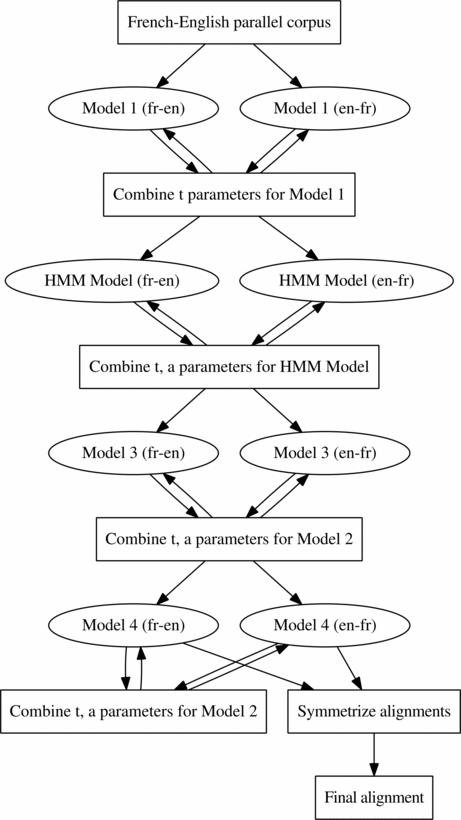
\includegraphics[width=0.6\textwidth]{images/symgiza.png}
\end{figure}

From all the available word aligning tools, such as GIZA++, MGIZA++, fast\_align~\cite{Dyer13}, etc., we decided to use SyMGIZA++. The results presented by its authors provide a convincing argument. They claim that the quality of the resulting alignment is increased by more than $17\%$ when compared to MGIZA++ or GIZA++, probably the most popular word alignment programs nowadays.

To train bilingual word vectors we need a parallel corpus together with its word alignment. In order to get the word alignment for the provided training corpus, we use SyMGIZA++. Furthermore, when running SyMGIZA++, the user can request the final values of the IBM Model 1 ``t'' parameters for both directions. In our method, these values are used to build the bilingual dictionary.

\section{bivec}
\label{section:bivec}

\textit{Word embedding} is a common name for a set of techniques which map words or phrases from a vocabulary to distributed word representations in the form of vectors consisting of real numbers in a high-dimensional continuous space. This section discusses bivec~\cite{Luong15}, a word embedding tool that creates bilingual word representations when provided with a word-aligned parallel corpus. The work is an extension of previous research, which resulted in a tool called word2vec~\cite{Mikolov13a}\cite{Mikolov13b}\cite{Mikolov13c}.

The original word2vec is a group of models producing monolingual word embeddings. These models are implemented as neural networks. They are trained to reconstruct the contexts of words. A monolingual corpus is needed for the training. During the training process, the algorithm iterates over the words in the corpus while considering the context of the current word in the form of a fixed-size window on its surrounding words. The two included models are:

\vbox{
\begin{itemize}
	\item The \textit{Continuous Bag-of-Words (CBOW)} model, trained to predict the word when given its context (without the current word).
	\item The \textit{Skip-gram (SG)} model, trained to predict the context of a given word.
\end{itemize}
}

\begin{figure}[!htb]
	\centering
	\caption{Continuous Bag-of-Words model (Source:~\cite{Rong14})}
	\label{figure:word2vec_cbow}
	\vspace{1em}
	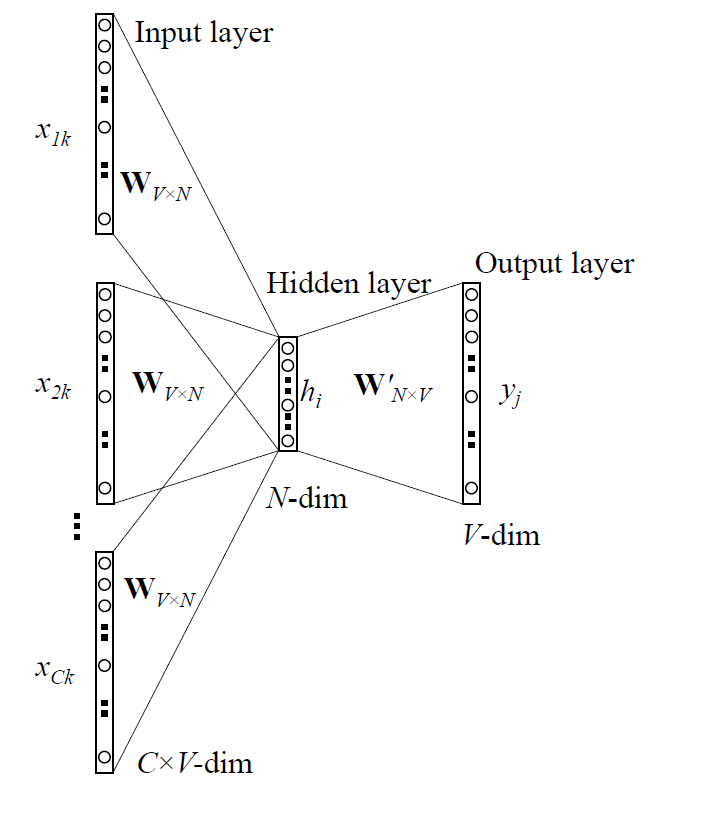
\includegraphics[width=0.6\textwidth]{images/word2vec_cbow.png}
\end{figure}

\begin{figure}[!htb]
	\centering
	\caption{Skip-gram model (Source:~\cite{Rong14})}
	\label{figure:word2vec_sg}
	\vspace{1em}
	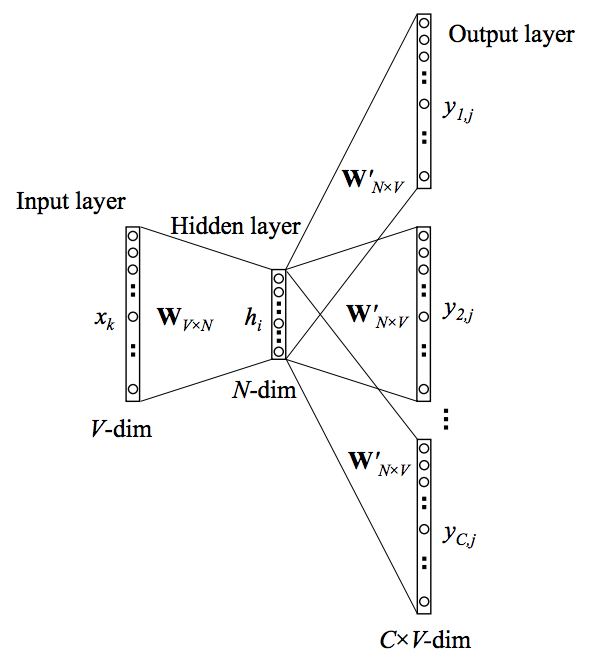
\includegraphics[width=0.6\textwidth]{images/word2vec_sg.png}
\end{figure}

The main difference between these two models can be observed in Figure~\ref{figure:word2vec_cbow} and Figure~\ref{figure:word2vec_sg}, which illustrate the structures of their underlying neural networks. When working with these networks, all the words are encoded to so-called one-hot vectors. This means that if $w_0, w_1, \ldots, w_V$ are all the unique words of the training corpus, word $w_i$ is encoded to a $V$-dimensional vector, where the $i$-th element is $1$ and all other $0$s.

In Figure~\ref{figure:word2vec_cbow}, one can see the one-hot vectors $x_{1,k}, x_{2,k}, \ldots, x_{C,k}$, representing the context of the current word in the input layer. In this model, the output layer consists of the one-hot vector of the word, $y_j$. On the other hand, Figure~\ref{figure:word2vec_sg} displays the one-hot vector of the word $x_k$ in the input layer, while the output layer contains the one-hot vectors of the words in its context, $y_{1,j}, y_{2,j}, \ldots, y_{C,j}$. In both these models, the user can choose the dimension of the hidden layer $N$ and the size of the context $C$. After the model is trained, it is used to map each of the words in the corpus to a vector. This vector is obtained from the hidden layer of the network and it represents the word's relationship with other words. The more the two words $w_i$, $w_j$ appear in the same context, the larger the \textit{cosine similarity} of their vectors $\operatorname{vec}(w_i)$, $\operatorname{vec}(w_j)$ is. Given two vectors $x$ and $y$, the cosine similarity is calculated as follows:

\begin{align*}
\operatorname{cos}(\textbf{x}, \textbf{y})=\frac{\textbf{x}\times\textbf{y}}{\lVert\textbf{x}\rVert\lVert\textbf{y}\rVert}= 
\frac{\sum\limits_{i=1}^{n} \textbf{x}_i\textbf{y}_i}{\sqrt{\sum\limits_{i=1}^{n} \textbf{x}_i^2} \sqrt{\sum\limits_{i=1}^{n} \textbf{y}_i^2}}.
\end{align*}

Word vectors obtained by training word2vec models have several interesting features. The relationship among the words are projected onto their vectors to such an extent, that for example the most similar vector to the resulting vector of an operation $\operatorname{vec}(\text{``king''}) - \operatorname{vec}(\text{``man''}) + \operatorname{vec}(\text{``woman''})$ is the vector $\operatorname{vec}(\text{``queen''})$. We will not pay further attention to more details about the advanced features of the word2vec results as they are not used in our method. It is worth mentioning that there are other related tools to word2vec, like for example GloVe~\cite{Pennigton14}.

The authors of bivec proposed an extension of the original Skip-gram model in the form of a joint bilingual model called the \textit{Bilingual Skip-gram (BiSkip)} model. When trained, this model can predict the context of a given word in both languages. In order to train, bivec requires a sentence-aligned parallel corpus and its word alignment. In fact, the word alignment is not strictly necessary, and if it is not provided, the system uses a simple heuristic. However, with the alignment provided, the results are better.

The most important idea behind the BiSkip model is the method of training. To gain insight into how the training works, let us look at the example illustrated in Figure~\ref{figure:bivec_bsg}. Suppose that we have two parallel sentences with their word alignment that says the English word ``trade'' is aligned with the German word ``Handels-''. We can use the associated German word ``Handels-'' to predict the surrounding English context containing the words like ``economic'' and ``financial''. Generally speaking, given a word $w_1$ in a language $l_1$, and a word $w_2$ in a language $l_2$ aligned to $w_1$, the BiSkip model uses the word $w_1$ to predict not only its own context in $l_1$, but also the context of the word $w_2$ in $l_2$. The other word $w_2$ is handled analogously. This results in training of a single Skip-gram model with a joint vocabulary on parallel corpora. In other words, BiSkip model is like a single Skip-gram model trained jointly to predict words for each of the language pairs $l_1 \rightarrow l_1$, $l_1 \rightarrow l_2$, $l_2 \rightarrow l_1$, and $l_2 \rightarrow l_2$ simultaneously. The resulting vector representations have the same properties, except that in this case they appear not only monolingually but also cross-lingually. It means, for example, that given a big enough English--German parallel corpus, the resulting vector representations of the words ``car'' and ``Auto'' would have greater cosine similarity.

\begin{figure}[!htb]
	\centering
	\caption{Bilingual Skip-gram model (Source:~\cite{Luong15})}
	\label{figure:bivec_bsg}
	\vspace{1em}
	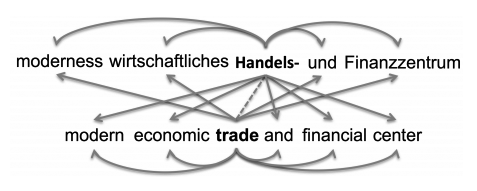
\includegraphics[width=0.6\textwidth]{images/bivec_bsg.png}
\end{figure}

Similarly to word2vec being not the only one among the monolingual word embedding strategies, bivec also has some interesting relatives. We could mention BilBOWA~\cite{Gouws14} (Bilingual Bag-of-Words without Alignments), a simple and computationally efficient model, which also learns bilingual distributed representations of words. The method does not require word alignment; instead, it trains directly on monolingual data using extracted bilingual signal from a potentially smaller sentence-aligned parallel corpus.

We decided to use bivec for learning the bilingual word vectors from the training parallel corpus. The results conducted by the authors suggest that bivec achieved state-of-the-art results among other similar approaches when applied in the field of cross-lingual document classification. Using the trained bilingual word vectors and the proper weighting scheme, our method calculates the aggregate document vectors. The similarities among the word vectors are reflected in the document vectors; therefore, a pair of parallel documents have similar vectors.

\section{Annoy}
\label{section:annoy}

Annoy~\cite{annoy} is a C++ library with Python bindings implementing the \textit{approximate-nearest-neighbors (ANN)} search. The \textit {nearest-neighbor (NN)} search is an optimization problem defined as follows: given a set of points $S$ in a $d$-dimensional space $M$ and a query point $q \in M$, find the closest point in $S$ to $q$. A generalization of this problem is the \textit{k-nearest-neighbors (k-NN)} search, where we want to find the $k$ closest points. The NN and k-NN searches require the results to be optimal. Even the best algorithms to solve these problems are computationally demanding in terms of time. However, certain applications do not require the optimal solution to be found; they just need a result that would be ``good enough''. In ANN search, the algorithm does not guarantee to find the optimum, but in many cases it actually does. This relaxation enables the ANN algorithms to use less resources than the k-NN strategies would need. In particular, it takes less time to find the approximate neighbors, which is what we need in our method.

There are multiple libraries implementing the ANN search. When deciding which one to choose, we were inspired by the results of the available benchmarks~\cite{Bernhardsson16}. Annoy is fast and it is also user-friendly. It was developed during the Hack Week event at the company called Spotify\footnote{\url{https://www.spotify.com} (accessed April 11, 2016)}, where it is being used to create an index for billions of feature vectors representing individual songs. This index is distributed and searched in parallel to provide music recommendations for the users.

Annoy has several useful features. First of all, the user can choose between two different metrics: Euclidean distance and angular distance. The latter one is explained by the authors to actually mean Euclidean distance of normalized vectors. The testing results show that Annoy works better with less than $100$ dimensions, but the results are still efficient with less than $1,000$ dimensions. The library decouples index creation from lookup. The index needs to be built on a single machine and cannot be altered afterwards. After adding new items, the whole index needs to be rebuilt. The library allows storing the index to a file and also loading it from a file into memory. This feature enables building the index once and sharing it across all nodes in a cluster. This way, the index can be used in parallel execution. At this moment, we are not using the library in parallel execution; however, this feature may help to improve our system in the future.

In the background, Annoy uses random projections~\cite{Charikar02}\cite{Andoni08} to build up a forest of search trees---an index structure for the searching process. The algorithm for building the index uses SimHash, which is a locality-sensitive hashing (LSH) method. LSH is a family of hashing algorithms that perform dimensionality reduction of high-dimensional data. These algorithms hash items in such a way that similar ones end up close to each other, i.e.\ in the same buckets, with relatively high probability.

We use Annoy in our method to approximate the search fo parallel documents. We already know that a pair of parallel documents have similar document vectors. Therefore, in order to search for the parallel document we can perform the nearest-neighbour search in the set of document vectors associated with the other language. In our opinion, the task of refining parallel data from the web is not the kind of task that would require an algorithm to provide a perfect recall. When it comes to processing web-scale amounts of data, one must accept certain trade-offs. We believe that by preferring ANN to k-NN we can achieve an acceptable speed of the process and, eventually, more desirable results. 

\section{PyBrain}
\label{section:pybrain}

PyBrain~\cite{Schaul10} (Python-Based Reinforcement Learning, Artificial Intelligence and Neural Network Library) is a popular machine learning library for Python. It provides a flexible, easy-to-use, yet powerful algorithms for common machine learning tasks.

There is a part of our method, where we need to perform a binary classification task: whether to accept the pair of documents as parallel or not. As there are multiple features available for the task, it is hard to set up reasonable thresholds manually. Therefore we decided to use the classification provided by the feed-forward neural networks~\cite{Sima96}. For this purpose we use the neural network algorithms provided by the PyBrain library. 

The model of neural network used in our method is multilayer perceptron learning through the mechanism of backwards error propagation (backpropagation)~\cite{Rumelhart86}. This kind of model is widely popular and it is suitable for the type of classification task the method is facing.

\section{Common Crawl}
\label{section:common_crawl}

In Section~\ref{section:mining_common_crawl}, we have discussed the previous work concerning refining parallel corpora from Common Crawl dataset. The following text provides additional information about the dataset. The Common Crawl Foundation~\cite{CommonCrawl} is a non-profit organization with an aim of democratizing access to web information. They produce and maintain an open repository containing web-crawled data freely available for the public to use. 

The underlying infrastructure of Common Crawl uses Apache Nutch\footnote{\url{http://nutch.apache.org/} (accessed April 7, 2016)} as the primary web-crawling engine since 2013. Nutch runs in the form of Hadoop MapReduce jobs, which perform most of the core work of fetching pages, filtering and normalizing URLs and parsing responses to plug-ins. The plug-in architecture of Nutch allows the Common Crawl organization to make all the customizations they need, without maintaining a separate branch of the Nutch project. The infrastructure regularly crawls at aggregate speed of $40,000$ web pages per second. The performance is largely limited by the politeness policy, which the organization follows to minimize the impact on web servers the system crawls.

The time to release a new dataset (crawl) varies between one month to a quarter of year. Each crawl covers billions of web pages and takes hundreds of terabytes (TB) of disk space in an uncompressed form. Table~\ref{table:common_crawl} lists few of the crawls, along with their uncompressed size and number of contained pages.

\begin{table}[!htb]
	\centering
	\caption{Common Crawl dataset sizes}
	\label{table:common_crawl}
	\vspace{1em}
	\begin{tabular}{|l|r|r|}
		\hline
		\textbf{Crawl} & \textbf{Size (TB)} & \textbf{Pages (Billions)} \\
		\hline
		April 2015 & 168 & 2.11 \\
		May 2015 & 159 & 2.05 \\
		June 2015 & 131 & 1.67 \\
		July 2015 & 149 & 1.84 \\
		August 2015 & 106 & 1.32 \\
		\hline
	\end{tabular}
\end{table}

The crawls are hosted by the Amazon Web Services\footnote{\url{https://aws.amazon.com/} (accessed April 4, 2016)} as a part of the Public Data Sets\footnote{\url{https://aws.amazon.com/public-data-sets/} (accessed April 8, 2016)}. They are stored in a Simple Storage Service (S3)\footnote{\url{https://aws.amazon.com/s3/} (accessed April 8, 2016)}. The service allows the user to download the whole crawls to a local cluster. There is also a possibility to work with the datasets using the Amazon services, but these are paid. The Common Crawl foundation provides the users with the latest crawls in 3 different data formats:

\begin{itemize}
	\item The \textit{WARC}~\cite{WARC} (Web ARChive) format represents the raw archive of the crawl. It is a container for storing web content together with the associated network connections. It consists of series of records. There are three types of records: HTTP request, HTTP response and metadata describing the crawl process. Unlike the other two, it keeps the original HTML structure of the responses.
	
	\item The \textit{WAT} (Web Archive Transformation) format contains metadata extracted from the WARC records formatted in JSON~\cite{JSON}. These provide information such as content length, timestamp, mime type and URL.
	
	\item The \textit{WET} (WARC Encapsulated Text) format includes extracted plain text from the archived documents in WARC along with some basic metadata such as timestamp and URL.
\end{itemize}

Our other experiment uses realistic and noisy data from the July 2015 crawl. For the experiment, we have downloaded all the WARC files to our cluster, to be processed in our environment. We use the WARC format, because unlike the WET format it holds also the original HTML structure for the stored web pages. Using the HTML structure, we are able to extract paragraphs reliably. We consider these paragraphs as an input documents to be aligned.

\section{Hadoop}
\label{section:hadoop}

Common Crawl datasets belong to the category of Big Data~\cite{Holubova15}. When processing hundreds of terabytes large datasets, one definitely needs a more complex infrastructure and parallel processing paradigm. Apache Hadoop\footnote{\url{http://hadoop.apache.org/} (accessed April 9, 2016)}~\cite{White15} is an open-source Java-based~\cite{Gosling14}\cite{Lindholm14} software framework, which provides distributed storage along with means for distributed processing. It is designed to process large datasets on computer clusters built from commodity hardware. Hadoop is based on ideas originating in Google that invented an infrastructure able to process the data from the web at a large scale. The original distributed storage was called the Google File System~\cite{Ghemawat03} and the processing framework was named MapReduce~\cite{Dean04}. In the beginning, Hadoop was developed by employees of Yahoo! company as a part of the Apache Nutch project. Later it was separated to a standalone project.

Today, Hadoop is composed of many different components working together on a single platform. Historically, there are two main components in Hadoop. The storage for the data called HDFS (Hadoop Distributed File System)~\cite{Shvachko10} and computational framework for parallel executions---MapReduce. 

\subsection{HDFS}
\label{subsection:hdfs}

HDFS~\cite{hdfs_architecture} is a scalable storage, which enables user to store large files to a cluster in a distributed manner. It has a master/slave architecture illustrated in Figure~\ref{figure:hdfs_architecture}. An HDFS cluster has a master server, called NameNode. It manages the file system namespace and regulates file access rights. Moreover, there is a number of slaves, named DataNodes, present within the cluster, usually one per node. Each of the DataNodes manages storage on its node. HDFS exposes the file system namespace allowing the user to store the data. The internal implementation splits a file into a group of blocks that are distributed across a set of DataNodes. This allows huge files to be stored. The NameNode determines the mapping of blocks to DataNodes. It is also responsible for operations like opening, closing and renaming of files and directories. The DataNodes serve read and write requests from clients. They also provide an interface for block creation, deletion and replication to the main NameNode. The mechanism of data replication is centrally managed by the NameNode.

\begin{figure}[!htb]
	\centering
	\caption{HDFS architecture (Source:~\cite{hdfs_architecture})}
	\label{figure:hdfs_architecture}
	\vspace{1em}
	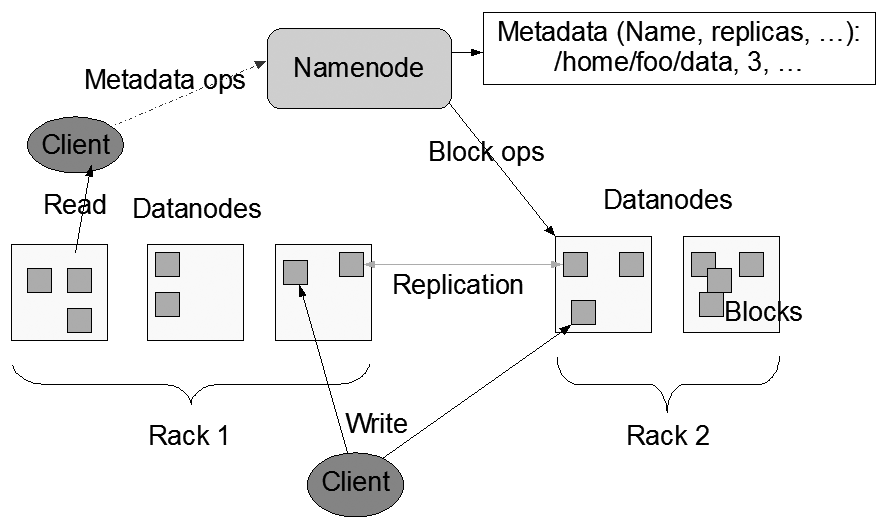
\includegraphics[width=0.8\textwidth]{images/hdfs_architecture.png}
\end{figure}

\subsection{MapReduce}
\label{subsection:mapreduce}

MapReduce~\cite{mapreduce_tutorial} is a software framework, which allows to process vast amounts of data on large clusters. It is reliable and fault-tolerant. A MapReduce job splits the input data into independent chunks. These are first processed in parallel by the map tasks (mappers). With map tasks finished, the framework sorts their output and the results are passed to the reduce tasks (reducers). The framework is responsible for scheduling, monitoring and re-execution of the tasks. In a typical scenario, the MapReduce framework and HDFS are running on the same set of nodes. This configuration allows the framework to effectively schedule the tasks to nodes where the data reside. This way, the system minimizes the amount of network traffic needed for job execution. Similarly to HDFS, also MapReduce has a master/slave architecture. The framework consists of a single master ResourceManager, multiple NodeManagers (one per node of a cluster), and one MRAppMaster per application. The framework application has to specify the input and output locations and supply the implementations for the map and reduce tasks. These and other settings form a job configuration. The process starts when a job client submits a job with a JAR file (Java Archive) or executable to the ResourceManager. The ResourceManager then distributes the software and configuration to the slaves and begins scheduling the tasks. During the execution, it provides status and diagnostic information. 

The framework operates exclusively using \textit{key-value} pairs. It is a fundamental data structure providing users with extensibility. In a key-value based data model the information is stored within collections in which every item is a pair of key and value. Within the framework, the input of a job is a set of key-value pairs. The output of the job is another set of key-value pairs of possibly different types. The classes of keys and values need to be serializable by implementing a dedicated interface. Additionally, the key classes need to be comparable. The standard dataflow of the MapReduce job execution is following:

\begin{enumerate}
	\item The system first divides the input data into splits. These splits have usually 64--128 megabytes (MB). The framework assigns one split to each mapper. Then it begins to read the input data from the HDFS, generating key-value pairs. These pairs are passed to the mappers. In a typical case, if processing plain text files, a key-value pair would be generated for each line in every file located in an input directory.
	
	\item The mapper gets a series of key-value pairs. While processing one input pair it can generate zero or multiple output key-value pairs. The types of input and output keys and values may differ. 
	
	Listing~\ref{listing:wordcount_map} shows an pseudo-code implementation of a map function from the classical WordCount example which performs extraction of word frequencies. In this case the function is called for every line contained in the assigned split. The mapper gets the line and divides it into its words. Then for each of these words it emits an output key-value pair, where key is the word and value is 1. The value represents a single occurrence of the word.

	\item Every output of each mapper is assigned to a specific reducer. The partition function gets the mapper output key and the actual number of reducers and it determines the associated reducer. Then the data are shuffled---they are sorted in parallel, using the provided comparison function, and exchanged between the nodes of mappers and reducers. The performance of this phase is dependent on the speed of the network between cluster nodes.
	
	\item For each unique key, in sorted order, a reducer is called. Reducer iterates over all the values associated with the given unique key. It can generate zero or multiple output key-value pairs. Like in mapper, also in reducer the types of input and output keys or values may differ.
	
	The implementation of a reduce function from the word count example is presented in Listing~\ref{listing:wordcount_reduce}. It sums all the partial counts emitted by mappers into a total count for each of the unique words.
	
	\item Finally, the system stores the output of the reducers to the HDFS. The framework allows the user to define MapReduce batch jobs for executing multiple jobs in a sequence.
\end{enumerate}

\begin{lstlisting}[float=htb!,language=bash,caption={WordCount: map},label={listing:wordcount_map}]
function map(String name, String line):
	for word in line.split():
		emit(word, 1)
\end{lstlisting}

\begin{lstlisting}[float=htb!,language=bash,caption={WordCount: reduce},label={listing:wordcount_reduce}]
function reduce(String word, Iterator partial_counts):
	total_count = 0
	for count in partial_count:
		total_count += count
	emit(word, total_count)
\end{lstlisting}

In order to store and process the July 2015 dataset of the Common Crawl (149 TB, 1.84 billions of pages), we needed a distributed storage and framework for parallel data processing. Therefore, we decided to use the Apache Hadoop for these purposes. When wondering about other means of processing of such a huge dataset, one can get inspired by the list of example projects using Common Crawl data\footnote{\url{http://commoncrawl.org/the-data/examples/} (accessed April 10, 2016)}. One of the examples mentioned in the list is the method described in Chapter~\ref{chapter:related_work}.

\section{WARC-Hadoop}
\label{section:warc_hadoop}

When processing data in a custom format (e.g.\ WARC file format) with Hadoop, the user needs to implement a set of interfaces for the system to handle the data properly. There exist a number of libraries which enable Hadoop to process the WARC files with the MapReduce framework. We decided to utilize one such library, called warc-hadoop~\cite{warc-hadoop} in our experiment.

The warc-hadoop is a Java library providing the functionality for reading and writing WARC files in MapReduce environment. It also enables the framework to serialize and transfer individual WARC records while shuffling the data between the mappers and reducers. This library was created with an intention to help the users explore the content of the Common Crawl datasets.

\section{MetaCentrum}
\label{section:metacentrum}

The Hadoop cluster we use for our experiments is provided by the MetaCentrum\footnote{\url{https://www.metacentrum.cz/en/} (accessed April 10, 2016)} project, which is an activity of the CESNET\footnote{\url{https://www.cesnet.cz/?lang=en} (accessed April 10, 2016)} association. MetaCentrum operates and manages distributed computing infrastructure, which consist of computing and storage resources owned by CESNET and cooperating academic centers located in the Czech Republic. Moreover, MetaCentrum holds responsibility for building the National Grid and its integration with related international activities.

The provided Hadoop cluster in MetaCentrum consists of 3 management nodes and 24 worker nodes. The management nodes run components like front-end, HDFS NameNode and MapReduce History Server. Every node of the configuration has Intel\textregistered{} Xeon\textregistered{} CPU E5-2630 v3 (20 MB Cache, 2.40 GHz) and 128 gigabytes (GB) of memory. The overall disk space available on the cluster is 1.02 petabytes (PB). The HDFS operates with a replication factor of 4, which means that the cluster can hold de facto 261 terabytes (TB) of user data.

Access to computing and storage facilities owned by parties and projects contributing to the National Grid Infrastructure MetaCentrum, provided under the programme "Projects of Large Research, Development, and Innovations Infrastructures" (CESNET LM2015042), is greatly appreciated.

\section{jsoup}
\label{section:jsoup}

Processing data from the web is usually complicated. For example, there are many web pages, that do not have valid HTML structure or are encoded in different character sets. To tackle this we use a library called jsoup~\cite{jsoup}, a Java library for working with real-world HTML structures. It transforms the HTML structure to the Document Object Model (DOM)~\cite{DOM}.

The jsoup library provides a way to extract data using DOM traversal or Cascading Style Sheets (CSS) selectors. Furthermore it allows the user to clean the HTML structure by keeping only the HTML elements and attributes present in a provided whitelist.

In our real-world data experiment, we process Common Crawl dataset with the native Java MapReduce library. Therefore we consider jsoup as suitable library for our needs. We use the library in parallel execution environment to parse the HTML structures of the web pages. The library allows us to scrape the contents of the HTML elements \texttt{<p>} representing paragraphs of text that we consider as input documents to be aligned by our method. We could also collect content of other elements such as \texttt{<h1>}--\texttt{<h6>}, \texttt{<li>}, \texttt{<th>}, \texttt{<td>}, etc., as well.

\section{language-detector}
\label{section:language_detector}

Another Java library we use in our real-world data experiment is language-detector~\cite{language-detector}. As the name suggests, it is a library that performs language detection. It contains built-in profiles for 70 different languages, which were trained using common texts available for each of the languages. The library also allows the user to train a custom language profile when provided with a monolingual corpus. Underneath, the library uses N-gram-based text categorization~\cite{Cavnar94}. 

We use this library while running MapReduce over the Common Crawl dataset. For each of the paragraphs scraped from the web pages, we identify the language using the language-detector library. This way the MapReduce job is able to keep only the paragraphs in the languages of our interest.

%%%%%%%%%%%%%%%%%%%%%%%%%%%%%%%%%%%%%%%%%%%%%%%%%%%%%%%%%%%%%%%%%%%%%%%%%%%%%%%%
%% MASTER'S THESIS                                                            %%
%%                                                                            %% 
%% Title (en): Mining Parallel Corpora from the Web                           %%
%% Title (sk): Rafinácia paralelných korpusov z webu                          %%
%%                                                                            %%
%% Author: Bc. Jakub Kúdela                                                   %%
%% Supervisor: Doc. RNDr. Irena Holubová, Ph.D.                               %%
%% Consultant: RNDr. Ondřej Bojar, Ph.D.                                      %%
%%                                                                            %%
%% Academic year: 2015/2016                                                   %%
%%%%%%%%%%%%%%%%%%%%%%%%%%%%%%%%%%%%%%%%%%%%%%%%%%%%%%%%%%%%%%%%%%%%%%%%%%%%%%%%

\chapter{Proposed Method}
\label{chapter:proposed_method}

This chapter describes our solution to the task of bilingual document alignment. The method has been already outlined in Section~\ref{section:overview_of_proposed_method} of Chapter~\ref{chapter:background_work_and_prerequisities} containing an introduction to all the resources and tools used in our work. The following text discusses our method in a greater level of detail.

\section{Task Definition}
\label{section:task_definition}

Our method solves an extended version of the bilingual document alignment task. This version of the task can be defined as follows: let us assume we have a number of sets containing documents from both the languages of our interest. We call these sets \textit{bins}. Each bin represents a stand-alone set of input documents for the original task. The solution of this task is a collection of pairs of documents where each pair consists of two parallel documents from the same bin.

A bin can contain up to millions of documents and is not required to have a balanced language distribution. Individual bins may vary in size. The method does not align the documents either belonging to the different bins or having the same language. Intuitively, the smaller the size of bin, the better the quality of the resulting alignment. It also takes more time and memory to align a larger bin.

When mining bilingual parallel corpora from the web, one can form a bin for every identified bilingual web domain. Such a bin can contain all the paragraphs in both the languages, scraped from the domain. This way the method will consider aligning of all the paragraphs from the domain regardless of the URLs and HTML structures of its web pages.

\section{Training Part I: Dictionary, Word Vectors}
\label{section:method_training_1}

Our method is supervised and needs to be trained on an already existing sentence-aligned corpus for the language pair we are interested in. For better clarity, we distinguish between two parts of the training process. This section describes the first part of training, while the other part is described in Section~\ref{section:method_training_2}. When trained, Section~\ref{section:method_running} explains how the method aligns the input data.

Let us describe the first part of the training process as depicted in Figure~\ref{figure:method_1}. Within the diagram, rectangles represent data in various formats, ovals stand for processing steps and arrows symbolize the flow of the process. The objective of this part of the training, is to preprocess the training parallel corpus and create a bilingual dictionary together with bilingual word vectors. The process is described in the following text.

\begin{figure}[!htb]
	\centering
	\caption{Proposed method: training part I}
	\label{figure:method_1}
	\vspace{1em}
	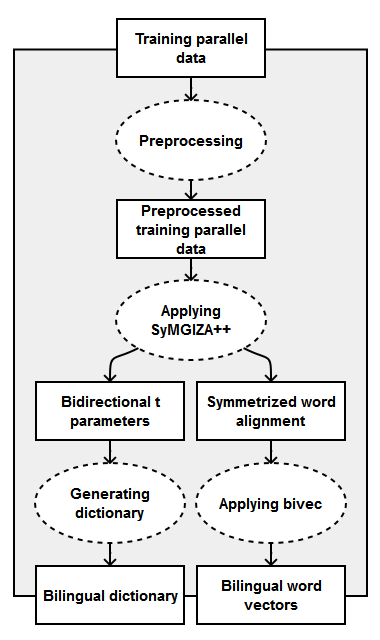
\includegraphics[width=0.50\textwidth]{images/method_1.png}
\end{figure}

\subsection{Preprocessing Training Parallel Data}
\label{subsection:preprocessing_training_parallel_data}

The procedure begins with preprocessing of the sentence-aligned training parallel corpus which may involve tokenization, lemmatization, stemming, truecasing, lowercasing, removing unknown symbols, removing stop words, etc. For individual language pairs, different preprocessing steps might help to gain better quality results. Any type of preprocessing done in this step needs be also applied to the input data, before the alignment process starts, for the method to work properly. However, this does not mean, that the user must end up with pairs of parallel documents in preprocessed format. The method is easily extensible to be able to track down the original documents. 

In our experiments with Czech--English language pair, the preprocessing includes either tokenization or lemmatization, followed by lowercasing. The tokenization and lemmatization is done utilizing MorphoDiTa (see Section~\ref{section:morphodita}), an open-source morphological dictionary and tagger.
	
\subsection{Applying SyMGIZA++}
\label{subsection:applying_symgiza}

The method follows the well-known recommendations to get a good-quality word alignment. The resulting corpus from the previous step is further cleaned by removing all the sentence pairs, where one of the sentences contains more than $50$ tokens or does not contain a single letter from any alphabet.

Then SyMGIZA++ (see Section~\ref{section:symgiza}) is executed to obtain the word alignment for the preprocessed and cleaned training parallel corpus. This step includes preparation of word classes and word co-occurrences which are used in the alignment process. The results of the execution include the values of the IBM Model 1 ``t'' parameters, after its last iteration, for both directions.

\subsection{Generating Dictionary}
\label{subsection:generating_dictionary}

The bilingual dictionary is built using the final IBM Model ``t'' parameters estimated by SyMGIZA++. The algorithm is the same as the one implemented in Bitextor's script for creating a custom dictionary (see Section~\ref{section:bitextor}). Each word pair that appears in both directions and has the harmonic mean of the ``t'' parameters (i.e.\ \textit{weight}) great enough, is included into the dictionary. Unlike the Bitextor's one, this type of a dictionary includes also the weights.

We created a script \texttt{merge\_param.py} which takes the SyMGIZA++ vocabulary files for both languages, files containing ``t'' parameters for both directions, a threshold for the weights and produces a bilingual dictionary. Listing~\ref{listing:train_dictionary} shows a sample from the file containing bilingual dictionary created by this script.

\begin{lstlisting}[float=!htb,caption={Sample from a file with bilingual dictionary (training)},label={listing:train_dictionary},firstnumber=170724]
řekl	said	0.448062
řekl	told	0.162753
řekl	say		0.0364408
řekl	tell	0.0109902
\end{lstlisting}

By default, we keep all the pairs of words with weight more than $0.00001$. The threshold is set relatively low, producing large dictionaries. Searching through a larger dictionary takes more memory and computational time which heavily affects the overall performance of the method. The reasoning behind such a low threshold is that we wanted to demonstrate the limits of our method's precision rather than its performance. Yet, we consider the chosen threshold as still acceptable when talking about the resource requirements of the method.

\subsection{Applying bivec}
\label{subsection:applying_bivec}

The input files for bivec (see Section~\ref{section:bivec}) training are obtained by vertically splitting SymGIZA++ output file \texttt{all.A3.final\_symal}. Each line of this file contains a pair of parallel sentences along with their word alignment in a format introduced by Pharaoh\footnote{\url{http://www.isi.edu/licensed-sw/pharaoh/} (accessed May 2, 2016)}, a machine translation decoder. 

It is worth noting that bivec was built to accept alignment format of Berkeley Aligner\footnote{\url{https://code.google.com/archive/p/berkeleyaligner/} (accessed April 13, 2016)}, which is another word alignment tool. To transform the Pharaoh format into the required one, all the dashes must be replaced with spaces.

The method follows the recommendations of how should be the training data preprocessed. All the sequences of numbers are replaced with a zero symbol and all the unknown symbols (e.g.\ non-printable Unicode characters) with the specially dedicated tag \texttt{<unk>}.

With all the input files for training prepared, bivec is executed to create the bilingual word vectors. It is set to generate vectors with $40$ dimensions. Listing~\ref{listing:train_bivec_cs} and Listing~\ref{listing:train_bivec_en} show samples taken from the files containing bilingual word vectors produced by bivec. Additionally, Table~\ref{table:bivec_word_similarities} lists a sample of cosine similarities between the word vectors. In the table, the order of the Czech and English words is the same, so the diagonal represents translations.

There is a reason, why we keep the number of dimensions relatively low. The word vectors are used to calculate the aggregate document vectors with the same number of dimensions. The document vectors are then indexed using Annoy (see Section~\ref{section:annoy}). The authors of Annoy suggest that the tool works best with number of dimensions less than $100$. On the other hand, the authors of bivec conducted the tests using $40$, $128$, $256$ and $512$ dimensions. We have decided to use the only number of dimensions suitable for Annoy that has been tested.

\begin{lstlisting}[float=!htb,caption={Sample from a file with Czech word vectors (training)},label={listing:train_bivec_cs},firstnumber=89]
řekl 0.610664 0.186801 0.586637 -0.305300 0.785947 -0.114462 -0.168189 -0.800271 0.761297 -0.286534 0.195719 -0.125131 -0.821144 0.049325 -0.603093 -0.183007 0.240985 0.083267 0.144988 -0.375526 0.269821 -0.266884 0.141238 0.163624 -0.385829 0.255967 -0.700835 0.451331 0.341263 0.333853 0.177087 -0.085332 -0.222975 0.753013 0.005252 0.023802 -0.520247 -0.062342 -0.485972 -0.216207
\end{lstlisting}

\begin{lstlisting}[float=!htb,caption={Sample from a file with English word vectors (training)},label={listing:train_bivec_en},firstnumber=64]
said 0.601102 0.260525 0.566347 -0.263702 0.673600 -0.114424 -0.137723 -0.704463 0.619913 -0.402364 -0.043697 -0.052677 -0.862785 0.107025 -0.665232 -0.119659 0.101142 -0.086549 -0.105953 -0.572788 0.379709 -0.309156 0.056748 0.016574 -0.131031 0.380851 -0.356606 0.340167 0.374560 0.466035 0.319632 -0.070731 -0.221821 0.630211 0.117143 0.033079 -0.416265 -0.012100 -0.469880 -0.166465
\end{lstlisting}

\begin{table}[!htb]
	\centering
	\caption{Sample of cosine similarities between word vectors}
	\label{table:bivec_word_similarities}
	\vspace{1em}
	\begin{tabular}{|c|ccccc|}
		\hline
		& \textbf{řekl} & \textbf{kočka} & \textbf{pes} & \textbf{káva} & \textbf{čaj} \\
		\hline
		\textbf{said} & \textbf{0.9522} & 0.4480 & 0.4403 & 0.4492 & 0.5440 \\
		\textbf{cat} & 0.4070 & \textbf{0.9383} & \textbf{0.8350} & 0.5053 & 0.5346 \\
		\textbf{dog} & 0.4950 & \textbf{0.7727} & \textbf{0.9328} & 0.3900 & 0.5582 \\
		\textbf{coffee} & 0.4682 & 0.4423 & 0.3880 & \textbf{0.8456} & \textbf{0.9041} \\
		\textbf{tea} & 0.5014 & 0.4202 & 0.4232 & \textbf{0.8129} & \textbf{0.9698} \\ 
		\hline
	\end{tabular}
\end{table}


\section{Training Part II: Classifier}
\label{section:method_training_2}

With the first part of the training done, the method has prepared the preprocessed training parallel corpus (see Section~\ref{subsection:preprocessing_training_parallel_data}), bilingual dictionary with weights (see Section~\ref{subsection:generating_dictionary}), and bilingual word vectors (see Section~\ref{subsection:generating_document_vectors}).

The second part of the training process is illustrated in Figure~\ref{figure:method_2}. The process is almost the same as the procedure of running the trained method. The difference is that in training, we are aligning a supervised dataset with the intention to train a binary classifier able to decide whether to accept a pair of documents as parallel or not. The trained classifier is then used when running the trained method on the input data. The following text describes the procedure of the second part of the training.

\begin{figure}[!htb]
	\centering
	\caption{Proposed method: training part II}
	\label{figure:method_2}
	\vspace{1em}
	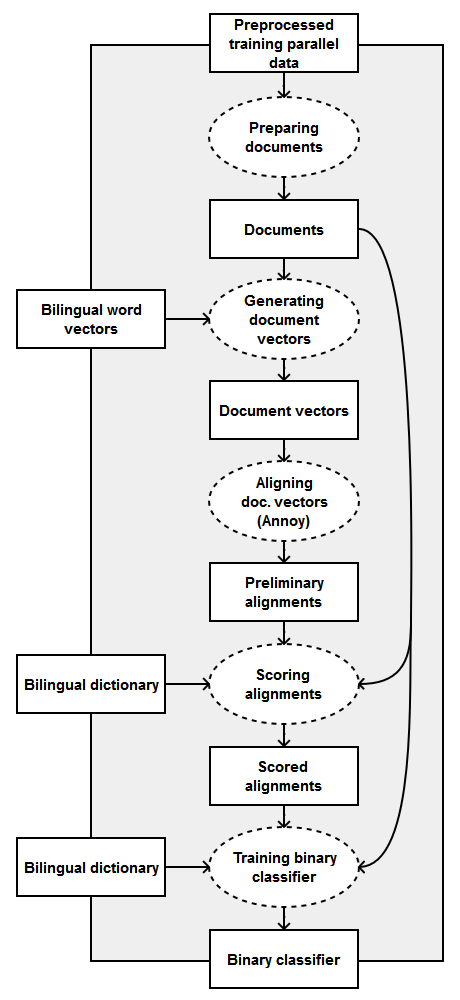
\includegraphics[width=0.60\textwidth]{images/method_2.png}
\end{figure}

\subsection{Preparing Documents}
\label{subsection:preparing_documents}

The first step creates the supervised dataset. The dataset consists of bins containing bilingual parallel documents. It is formed from the pairs of parallel sentences contained in the preprocessed training parallel corpus (see Section~\ref{subsection:preprocessing_training_parallel_data}). These are considered as pairs of parallel documents for the training.

In Section~\ref{section:task_definition}, we have explained the concept of the bins. The method splits all the pairs of documents into equally large bins (except the last one). The size of the bin should be an estimate of an expected size of the bin in a real-world dataset. In our experiment we split the documents into training bin consisting of $50,000$ pairs of parallel documents, i.e. $100,000$ documents. We consider this value as an upper-bound estimate of an average number of paragraphs in either of the two languages located on an ordinary bilingual web domain.

Our implementation accepts the supervised dataset in the form of two files, one for each language. Listing~\ref{listing:train_doc_cs} and Listing~\ref{listing:train_doc_en} show samples of such a pair of files. The format is a list of tab-separated values. The first column is an identifier of the bin. The samples show those parts of the files, where the first bin ends and the second bin starts. For the implementation to be able to iterate over both these files simultaneously, it is required that the bins are sorted in an alphabetic order. The second column is an identifier of the document. This identifier needs to be unique at least within the bin. The third column it the textual content of the document. The examples show documents from the tokenized and lowercased training parallel corpus. For the training to be successful, it is essential that each pair of parallel documents share the same bin and document identifier. This way the method knows which pairs of the documents are parallel.

\begin{lstlisting}[float=!htb,caption={Sample from a file with Czech documents (training)},label={listing:train_doc_cs},firstnumber=49999]
00000000	49998	" stál jsem támhle u zdi , " řekl .
00000000	49999	" nešpehoval jsem , harry .
00000001	50000	nikam nechodíme .
00000001	50001	pokračujte pane farbere .
\end{lstlisting}
	
\begin{lstlisting}[float=!htb,caption={Sample from a file with English documents (training)},label={listing:train_doc_en},firstnumber=49999]
00000000	49998	' i was standing there by the wall , ' he said .
00000000	49999	' i was n't spying , harry .
00000001	50000	we never socialize .
00000001	50001	continue , mr . farber .
\end{lstlisting}

\subsection{Generating Document Vectors}
\label{subsection:generating_document_vectors}

For each document, an associated vector is generated using the bilingual word vectors obtained in the first part of the training (see Section~\ref{subsection:applying_bivec}) together with the \textit{tf-idf} (term frequency-inverse document frequency) weighting scheme. The tf-idf weight of a term $d_i$ in a document $d=(d_1, d_2, \ldots,d_n)$ can be expressed as:

\begin{align*}
\operatorname{tf-idf}(d_i, d) = \operatorname{tf}(d_i, d) \times \operatorname{idf}(t) = \operatorname{tf}(d_i, d) \cdot \log \left(\frac{N}{\operatorname{df}(d_i)} \right)
\end{align*}

where $\operatorname{tf}(d_i, d)$ is the number of occurrences of the term $d_i$ in the document $d$, $\operatorname{df}(d_i)$ is the number of documents containing the term $d_i$, and $N$ is the number of all the documents in a dataset.

Our implementation processes both the files with documents one by one, bin by bin. When processing a bin, all the duplicate documents present in the bin are first discarded. Then, the inverse document frequencies are calculated for all the words that appear in the bin. Lastly, the document vector for every unique document $d=(d_1, d_2, \ldots, d_n)$ is generated as:
	
\begin{align*}
\operatorname{docvec}(d)=\sum\limits_{i=1}^{n} \operatorname{tf-idf}(d_i, d) \times \operatorname{wordvec}(d_i)
\end{align*}
	
where $\operatorname{wordvec}(d_i)$ is the word vector for the term $d_i$. The product operation in the formula is a multiplication of a scalar with a vector and the summation is derived from the operation of vector addition. If a word vector does not exist for a given term, a zero vector is used instead.
	
The described procedure is implemented in a script called \texttt{create\_docvec.py}. When given a file with documents and a file with word vectors for the associated language, it generates an output file containing document vectors. Listing~\ref{listing:train_docvec_cs} and Listing~\ref{listing:train_docvec_en} show a sample of its output. These lines contain the document vectors produced for the first pair of parallel documents displayed in Listing~\ref{listing:train_doc_cs} and Listing~\ref{listing:train_doc_en}. The output format of the script is very similar to the format of a file with documents. The only difference is that the document contents are replaced with document vectors.

\begin{lstlisting}[float=!htb,caption={Sample from a file with Czech document vectors (training)},label={listing:train_docvec_cs},firstnumber=49999]
00000000	49998	8.180257 -6.041753 6.456024 -7.385942 4.504289 -2.480280 -2.110008 -6.952853 9.294062 -5.956102 0.873277 0.288546 -8.055108 3.530353 -13.852273 1.189734 6.368119 4.307136 2.640194 -5.734687 -3.508690 -3.307812 -4.178317 -5.088661 -2.772588 10.505361 -7.485562 5.391955 5.723570 6.392571 3.516147 -1.386106 -5.184054 11.635170 -7.812555 6.185200 -0.854625 2.147744 -5.315508 1.234217
\end{lstlisting}

\begin{lstlisting}[float=!htb,caption={Sample from a file With English document vectors (training)},label={listing:train_docvec_en},firstnumber=49999]
00000000	49998	3.407737 -6.297829 7.404373 -6.480918 3.653056 0.363053 -0.486428 -4.324950 7.306768 -3.102215 -0.762884 -1.544800 -6.174080 0.820872 -10.864064 -1.982250 4.873059 -1.361170 -2.714015 -4.592477 2.429560 -1.330689 -4.640379 -3.568162 -1.444272 10.333115 -5.498119 1.396311 3.515478 9.095764 2.544416 -1.068039 -5.637783 5.594423 -3.433248 4.237183 0.336851 -0.263934 -2.851157 2.225453
\end{lstlisting}

\subsection{Aligning Document Vectors (Annoy)}
\label{subsection:aligning_document_vectors}

For each bin, the following procedure is performed. First, a search index is built containing the vectors of all the bins' documents in \textit{target language}. To build the search index, the method uses Annoy (see Section~\ref{section:annoy}) set to operate with the angular distance. Then, for every bin's document in the \textit{source language}, the index is searched to obtain $k$-approximate-nearest-neighbours to its vector. This returns a list of candidate parallel documents in the target language to the document in the source language. We call these preliminary alignments.

This procedure is implemented in a script called \texttt{align\_docvec.py}. When given files with the document vectors for both the languages, it creates an output file containing preliminary alignments. Listing~\ref{listing:train_align} shows a sample of its output. The first column is the bin identifier. The second and the third columns represent the identifiers of the documents in the source and the target language, respectively. The last column contains the similarity derived from the distance provided by Annoy calculated as $1-(d/2)$, where $d$ is the returned angular distance explained to be actually a Euclidean distance of normalized vectors. In the case presented in the sample, the parallel document ended as the 9\textsuperscript{th} best candidate (see line 4573319 in Listing~\ref{listing:train_align}).

\begin{lstlisting}[float=!htb,caption={Sample from a file with preliminary alignments (training)},label={listing:train_align},firstnumber=457311]
00000000	49998	44560	0.800532951951
00000000	49998	11723	0.791310846806
00000000	49998	9227	0.787315234542
00000000	49998	33875	0.781678438187
00000000	49998	18861	0.779217585921
00000000	49998	24646	0.771993637085
00000000	49998	9232	0.771212115884
00000000	49998	48420	0.770708605647
00000000	49998	49998	0.770486533642
00000000	49998	20284	0.768467396498
\end{lstlisting}

\subsection{Scoring Alignments}
\label{subsection:scoring_alignments}

Within the preliminary alignments, the top candidates are not necessarily the optimal ones. Therefore, the method applies a scoring function to reorder the candidates. This increases the probability of the optimal documents to appear higher in their candidate lists. Given the document $d=(d_1, d_2, \ldots,d_n)$ and its candidate $c=(c_1, c_2, \ldots, c_m)$, the scoring function is defined as:
	
\begin{align*}
\operatorname{score}(d, c)=\operatorname{length\_sim}(d, c) \times \operatorname{weight\_sim}(d, c)
\end{align*}
	
Both the functions $\operatorname{length\_sim}(d, c)$ and $\operatorname{weight\_sim}(d, c)$ have the range of $[0, 1]$. The idea is that the higher the result they return, the greater the possibility that the pair is parallel. These functions are defined as follows.

\begin{itemize}
	\item $\operatorname{length\_sim}(d, c)$ examines the ratio of the documents' lengths. It is based on the probability density function of the normal (Gaussian) distribution:
	
	\begin{align*}
	\operatorname{length\_sim}(d, c)=e^{-\dfrac{(\frac{\operatorname{len}(c)}{\operatorname{len}(d)}-\mu)^2}{2\sigma^2}}
	\end{align*}
	
	where $\frac{\operatorname{len}(c)}{\operatorname{len}(d)}$ is the actual ratio of the documents' lengths and $\mu$ is the expected ratio with the standard deviation $\sigma$. The expected ratio of documents's lengths with the associated standard deviation can be estimated using the pairs of parallel sentences from the preprocessed training parallel corpus. For the tokenized Czech--English parallel corpus these values are estimated to be $\mu_{cs \rightarrow en} \approx 1.08$ and $\sigma_{cs \rightarrow en} \approx 0.28$.
	
	\item $\operatorname{weight\_sim}(d, c)$ is based on the IBM Model 1~\cite{Brown93} and uses the bilingual dictionary created in the first part of the training. It is defined as:
	
	\begin{align*}
	\operatorname{weight\_sim}(d, c)=\prod\limits_{i=1}^{n} \sum\limits_{j=1}^{m} \frac{\operatorname{weight}(d_i, c_j)}{m}
	\end{align*}
	
	where $\operatorname{weight}(d_i, c_j)$ is the weight of the word pair $\langle d_i,c_j \rangle$ provided by the dictionary if the entry exists, otherwise it equals $10^{-9}$ (``null weight'').
\end{itemize}

A script called \texttt{score\_align.py} implements the described procedure. Given a file with preliminary alignments and files with the documents for both the languages, it creates an output file containing scored alignments. Listing~\ref{listing:train_score} shows a sample of its output. The output format is almost unchanged when compared with the format of a file with preliminary alignments. The only difference is that the similarity in the last column is replaced with the calculated score. The presented sample shows scored candidates from Listing~\ref{listing:train_align}. The matching document is now considered as the top candidate.

\begin{lstlisting}[float=!htb,caption={Sample from a file with scored alignments (training)},label={listing:train_score},firstnumber=457311]
00000000	49998	49998	1.21903368318e-14
00000000	49998	20284	9.19687934061e-20
00000000	49998	11723	1.55923045256e-23
00000000	49998	9232	9.73231577325e-25
00000000	49998	18861	7.95893854924e-27
00000000	49998	48420	8.82180461894e-28
00000000	49998	33875	1.19519536122e-30
00000000	49998	9227	1.70133029025e-38
00000000	49998	44560	2.16354386116e-43
00000000	49998	24646	9.5437947187e-55
\end{lstlisting}

\subsection{Training Binary Classifier}
\label{subsection:training_binary_classifier}

It is required from the binary classifier to be able to decide whether to accept a pair of documents as parallel or not. The chosen model for the classifier is a feed-forward neural network~\cite{Sima96}. The method uses an implementation provided by PyBrain (see Section~\ref{section:pybrain}). The classification is based on 4 features. All of these features have the range of $[0, 1]$. Given the document $d=(d_1, d_2, \ldots, d_n)$ and its candidate $c=(c_1, c_2, \ldots, c_m)$, the following list describes all the features.

\begin{itemize}
	\item $\operatorname{length\_sim}(d, c)$ has been already defined (see Section~\ref{subsection:scoring_alignments}). This function scores the ratio of the documents' lengths against the expected ratio.

	\item $\operatorname{length\_conf}(d, c)$ provides a supplementary information for the previous feature, which is not a reliable nor effective when scoring pairs of short documents; however, it is substantial when comparing pairs of long documents:
		
	\begin{align*}
	\operatorname{length\_conf}(d, c)=1 - e^{-0.01 \times \operatorname{len}(d)}
	\end{align*}
		
	This is a monotonically increasing function, that provides the model with an information of absolute length of the document $d$. The name of the feature is an abbreviation of ``length confidence'', which is justified by the fact that the higher the value of the $\operatorname{length\_conf}(d, c)$ is, the more authoritative is the score of the $\operatorname{length\_sim}(d, c)$.
		
	\item $\operatorname{weight\_sim_2}(d_i, c_j)$ is a modified version of $\operatorname{weight\_sim}(d, c)$ (see Section~\ref{subsection:scoring_alignments}). The original version was tested for the purposes of the classification, but the results were poor. This might be caused by the fact, that it returns very small values affected by the number of words contained in both the documents to a large extent. The modified version is defined as:

	\begin{align*}
	\operatorname{weight\_sim_2}(d, c)=\frac{\sum\limits_{i=1}^{n} \operatorname{len}(d_i) \times \max\limits_{j=1}^{m}\left(\operatorname{weight_2}(d_i, c_j)\right)}{\sum\limits_{i=1}^{n} \operatorname{len}(d_i) \times \operatorname{sgn}(\max\limits_{j=1}^{m}\left(\operatorname{weight_2}(d_i, c_j)\right))}
	\end{align*}
		
	where $\operatorname{weight_2}(d_i, c_j)$ is defined as the weight of the word pair $\langle d_i,c_j \rangle$ provided by the dictionary if the entry exists; however, if it does not exist and the two words are identical, then it equals $1$, otherwise it returns $0$.
		
	Let us explain the reason behind the heuristic of $\operatorname{weight_2}(d_i, c_j)=1$ for a pair of identical words not having entry present in the dictionary. The same set of features is used in the running process where occurrences of new words or special terms (e.g. URLs or email addresses) are expected. The heuristic considers a pair of identical words to be a perfect translation only if the dictionary does not contain other relation.
	
	Additionally, let us discuss why the weights are multiplied by the lengths of words. The assumption is that longer words are usually less frequent, carry more meaning and are therefore more important for the sentence, in contrast to short tokens (e.g. ``,'' or ``a''). The definition of $\operatorname{weight\_sim_2}(d, c)$ is an arithmetic mean of strongest relations between a source word from $d$ and any of the target words from $c$, weighted by the lengths of source words.

	Figure~\ref{figure:weight_sim} shows an example of $\operatorname{weight\_sim_2}$ calculation. In the example, for every source word in the Czech document, there exists an entry in the bilingual language dictionary with at least one of the target words from the English candidate document. Arrows represent the strongest among the relations ($\max\operatorname{weight_2}$) for each of the source words. The calculation above each of the source words is a multiplication of the length of the source word and the weight of the associated strongest relation.
\end{itemize}
		
\begin{figure}[!htb]
	\centering
	\caption{Example $\operatorname{weight\_sim_2}$ calculation}
	\label{figure:weight_sim}
	\vspace{1em}
	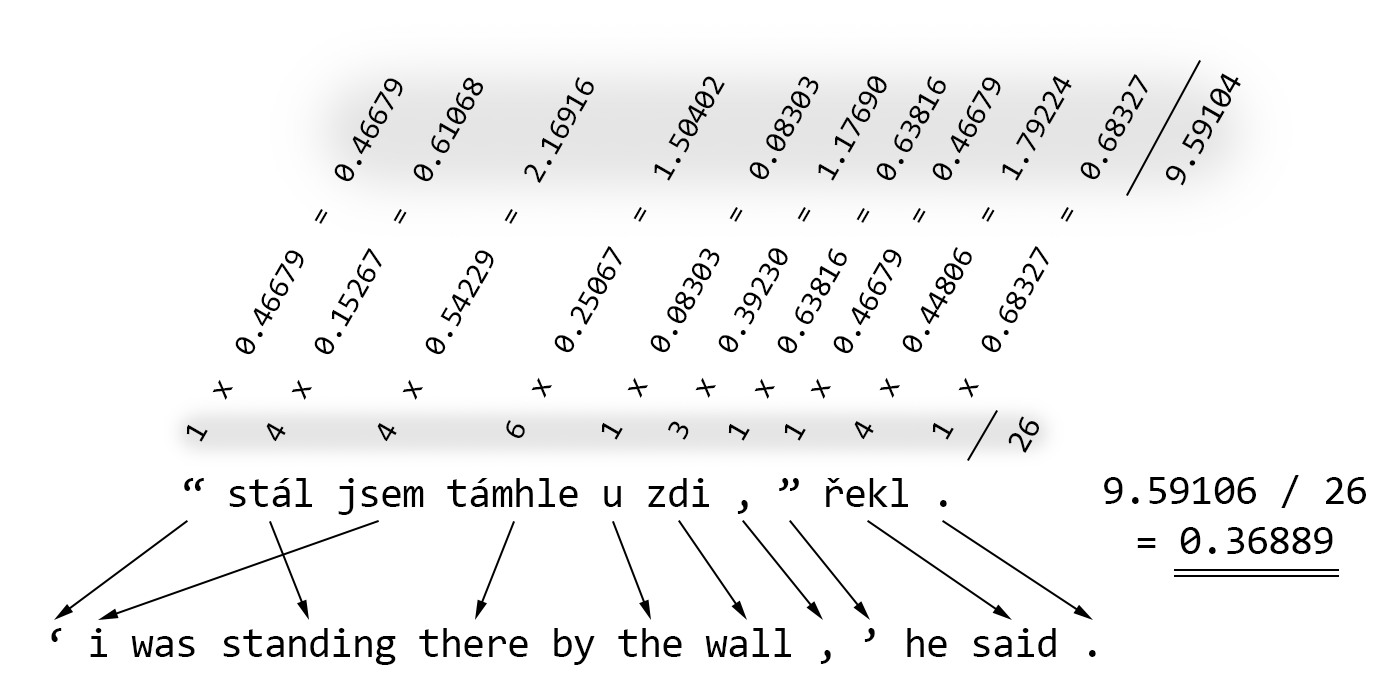
\includegraphics[width=0.8\textwidth]{images/weight_sim.png}
\end{figure}

\begin{itemize}[resume]
	\item $\operatorname{weight\_conf_2}$ is a supplementary feature for $\operatorname{weight\_sim_2}$. We can interpret the $\operatorname{weight\_sim_2}$ feature as: ``From what we know with the knowledge of possible incomplete dictionary, how likely are these two documents parallel?''. The supplementary feature can be similarly interpreted as: ``To what extent the dictionary covers the pairs of words we came across?''. The formal definition is following:
		
	\begin{align*}
	\operatorname{weight\_conf_2}(d, c)=\frac{\sum\limits_{i=1}^{n} \operatorname{len}(d_i) \times \operatorname{sgn}(\max\limits_{j=1}^{m}\left(\operatorname{weight_2}(d_i, c_j)\right))}{\sum\limits_{i=1}^{n} \operatorname{len}(d_i)}
	\end{align*}
\end{itemize}
	
With all the features designed for the classification defined, the process of training can be explained. It starts by creating a training dataset using the scored alignments. For every document $d$ in the source language and its top candidate $c$ in the target language the following pair of input$\rightarrow$output vectors is added into the training dataset:

\begin{align*}
\begin{pmatrix}
\operatorname{length\_sim}(d, c) \\
\operatorname{length\_conf}(d, c) \\
\operatorname{weight\_sim_2}(d, c) \\
\operatorname{weight\_conf_2}(d, c)
\end{pmatrix} \rightarrow \begin{cases}
\begin{pmatrix} 0 \\ 1 \end{pmatrix}, & \text{if } \langle d,c \rangle \text{ are parallel} \\\\
\begin{pmatrix} 1 \\ 0 \end{pmatrix}, & \text{otherwise.} \\
\end{cases}
\end{align*}

The input vector consists of the 4 defined features, while the output vector encodes whether the documents $\langle d,c \rangle$ are parallel or not. The first value of the output vector represents the probability of the documents to be non-parallel. The second value is complementary to the first.

Before the network is trained, the collected training dataset is subsampled to contain an approximately equal number of items representing parallel and non-parallel document pairs. This helps the network to be less affected by the ratio of parallel and non-parallel pairs. At this moment, it is also possible to reduce the size of the dataset to shorten the time it takes to complete the training.

This described procedure is implemented in a script called \texttt{train\_network.py}. When given a file with scored alignments and files with documents for both the languages, the script trains a network and stores its configuration to a disk on a requested location in the form of an XML file. This allows the method to load and use the trained network at any time. It also enables the system to distribute the trained model to other nodes.

\section{Running}
\label{section:method_running}

With the second part of the training done, the method has prepared a binary classifier able to decide whether to accept a pair of documents as parallel or not (see Section~\ref{subsection:training_binary_classifier}).

The process of running the trained method on the input data is illustrated in Figure~\ref{figure:method_3}. The resemblance between this process and the procedure of the second part of the training has been already discussed. Due to the large extent of similarity the shared parts of the process are described briefly as they have been discussed in detail in Section~\ref{section:method_training_2}.

\begin{figure}[!htb]
	\centering
	\caption{Proposed method: running}
	\label{figure:method_3}
	\vspace{1em}
	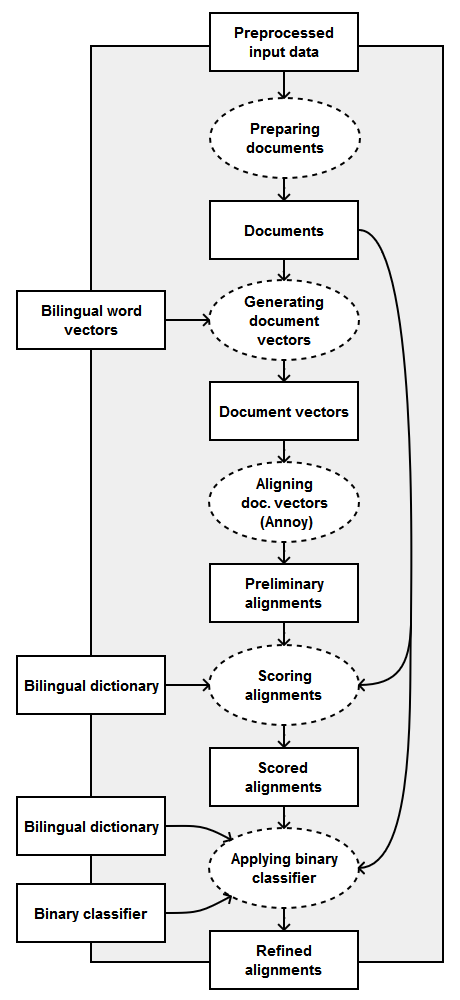
\includegraphics[width=0.60\textwidth]{images/method_3.png}
\end{figure}

\subsection{Preparing Documents}
\label{subsection:preparing_documents_running}

As mentioned earlier in Section~\ref{subsection:preprocessing_training_parallel_data}, the input documents have to be preprocessed in the same way as the training parallel corpus. Then, the preprocessed documents have to be split into bins. As already noted (see Section~\ref{section:task_definition}), when aligning paragraphs from the web, a bin can contain all the paragraphs for both the languages, scraped from one bilingual web domain. In this scenario, the names of the domains can be used as bin identifiers. This restricts the method to align only the paragraphs originating from the same domain. On the other hand, if aligning inseparable data, e.g. documents without a natural distribution into groups, all the documents can be placed into a single bin with an arbitrary identifier. However, the method has better recall when aligning smaller bins. This is caused mainly by Annoy, which has better accuracy when searching through an index with less items.

Our implementation accepts the input dataset in a form of two files, one for each language. It is the same format as for the supervised dataset, described in Section~\ref{subsection:preparing_documents}. Listing~\ref{listing:run_doc_cs} and Listing~\ref{listing:run_doc_en} show samples of such a pair of files containing Czech and English paragraphs acquired from the web.
	
\begin{lstlisting}[float=!htb,caption={Sample from a file with Czech documents (running)},label={listing:run_doc_cs},firstnumber=154290]
europa.eu	154289		v praze se fórum zaměřilo konkrétně na jadernou bezpečnost , politiky nukleárního odpadu , možné iniciativy v oblasti odborné přípravy a vzdělávání a transparentnosti .
\end{lstlisting}

\begin{lstlisting}[float=!htb,caption={Sample from a file with English documents (running)},label={listing:run_doc_en},firstnumber=1085753]
europa.eu	1085752		at the prague meeting the forum has been dedicated more particularly to nuclear safety , nuclear waste policies , possible initiatives on training and education as well as in the area of transparency .
\end{lstlisting}

\subsection{Applying Binary Classifier}
\label{subsection:applying_binary_classifier}

With the input dataset prepared, the process follows with the exact same steps applied to the supervised dataset in the second part of the training. First, vectors are generated for all the documents (see Section~\ref{subsection:generating_document_vectors}). Then, the document vectors are aligned by searching for nearest neighbours of all documents in the source language, resulting in preliminary alignments (see Section~\ref{subsection:aligning_document_vectors}) and these are subsequently scored (see Section~\ref{subsection:scoring_alignments}).

As a final step, the trained classifier (see Section~\ref{subsection:training_binary_classifier}) is used to obtain the refined alignments. For every document $d$ in the source language and its top candidate $c$ in the target language the trained network is activated as follows:

\begin{align*}
\begin{pmatrix}
\operatorname{length\_sim}(d, c) \\
\operatorname{length\_conf}(d, c) \\
\operatorname{weight\_sim_2}(d, c) \\
\operatorname{weight\_conf_2}(d, c)
\end{pmatrix} \xrightarrow{?} \begin{pmatrix} a \\ b \end{pmatrix}
\end{align*}
	
The input vector contains the same set of features as in the training. When activated, the second value from the output vector $b \in [0, 1]$ represents the confidence of a prediction that the two documents $\langle d,c \rangle$ are parallel. If the confidence $b$ is greater than a user-defined threshold, the document pair $\langle d,c \rangle$ ends up in the resulting refined alignments.

A script called \texttt{apply\_network.py} implements the described procedure. When given a file containing the network configuration of a classifier, a file with scored alignments and files with documents for both the languages, it creates an output file containing refined alignments. Listing~\ref{listing:run_refine} shows a sample of its output. The output format follows the convention of the files with preliminary and scored alignments. This time, the last column represents the confidence returned by the classifier. The presented sample shows that the two paragraphs from Listing~\ref{listing:run_doc_cs} and Listing~\ref{listing:run_doc_en} are successfully aligned.

\begin{lstlisting}[float=!htb,caption={Sample from a file with refined alignments (running)},label={listing:run_refine},firstnumber=33683]
europa.eu	154289	1085752		0.9996949388
europa.eu	154287	1085750		0.999479551945
europa.eu	154284	1163960		0.996325842675
europa.eu	154285	1163962		0.996881020525
\end{lstlisting}
\section{Discussion}
\label{section:method_discussion}

The second part of the training process and its resemblance to the procedure of running the trained method may seem cumbersome. However, in case of presence of a different binary classifier able to tell whether the two documents are parallel or not, the whole second part of the training could be excluded and the provided classifier would be utilized.

An alternative classifier could be based on a pre-trained SMT system that would be used to translate the document in the source language into the target one to be compared with the other document. This idea was adapted in the related project focused on mining Wikipedia (see Section~\ref{section:mining_wikipedia}).

Our classifier is more similar to the one used by STRAND (see Section~\ref{section:strand}). The STRAND's classifier is based on a decision tree built over a set of features comparing the similarity between a pair of potentially parallel HTML structures. In contrast to this, our method uses a neural network trained with a set of features designed to compare two potentially parallel plain text documents.

In our method, the second part of the training process simulates the aligning of a supervised dataset with the knowledge of the optimal solution. In the end of the procedure, the model of the classifer is trained. This is a generic approach that can be easily modified. One can redesign the set of features for the classification or completely change the implementation of the learning model.

Inspired by STRAND's classifier, we tried to swap the neural network model with a model based on a decision tree using the same set of features. For these purposes, we used the implementation provided by Scikit-learn~\cite{Pedregosa11}, a Python machine learning library. The tentative results were poorer; however, we did not spend that much time with trying different parameters and testing.

It is important to note, that the method, in its present form, does not take into account the order of the words when aligning parallel documents. The tf-idf weighting scheme, the scoring function based on the IBM Model 1 and even all the features used by the classifier completely ignore this aspect. Despite the fact that the results are promising, there are places for improvement.

It is also important to highlight the fact that our method is asymmetric regarding the fact that it generates different results if the source and the target languages are swapped. The main reason behind this is that the document vectors associated with the target language are indexed by Annoy while the other vectors for the source language are used as query points for the approximate-nearest-neighbours search. From our experience, a rule of thumb is to choose the language with more documents to be the target one.

The method is designed to be able to run in parallel or distributed environment. Bins with input documents represent independent isolable tasks. These can be distributed across multiple nodes together with the once trained resources needed for the execution. These include bilingual dictionary, bilingual word vectors and the trained classifier.

The key idea behind our method is to use the combination of bilingual word embedding and locality-sensitive hashing. Usually the most expensive operation when solving the task of document alignment is the content comparison of the two documents. A naive approach compares each of the $N$ documents in the source language, with all the $M$ documents in the target language resulting in $N \times M$ comparisons. Our method reduces this number to $N \times k + N$. The $N \times k$ is the number of comparisons needed for the scoring of the $k$ candidates from all the possible $M$ ones as returned by the approximate-nearest-neighbours search and $N$ is the number of comparisons necessary for the final classification of the top candidates.
%%%%%%%%%%%%%%%%%%%%%%%%%%%%%%%%%%%%%%%%%%%%%%%%%%%%%%%%%%%%%%%%%%%%%%%%%%%%%%%%
%% MASTER'S THESIS                                                            %%
%%                                                                            %% 
%% Title (en): Mining Parallel Corpora from the Web                           %%
%% Title (sk): Rafinácia paralelných korpusov z webu                          %%
%%                                                                            %%
%% Author: Bc. Jakub Kúdela                                                   %%
%% Supervisor: Doc. RNDr. Irena Holubová, Ph.D.                               %%
%% Consultant: RNDr. Ondřej Bojar, Ph.D.                                      %%
%%                                                                            %%
%% Academic year: 2015/2016                                                   %%
%%%%%%%%%%%%%%%%%%%%%%%%%%%%%%%%%%%%%%%%%%%%%%%%%%%%%%%%%%%%%%%%%%%%%%%%%%%%%%%%

\chapter{Prealigned Data (CzEng) Experiment}
\label{chapter:prealigned_data_czeng_experiment}

This chapter describes the first experiment conducted with our method. The experiment involves the prealigned parallel data. This type of data enable us to automatically compare the method's results with the original alignment. Therefore, we can estimate the effectiveness of the proposed method.

For the experiment, we have selected Czech--English language pair. The most important reasons behind this selection are that we can use the available Czech--English parallel data and we understand both these languages well. The parallel corpus used for this experiment consists of all the training sections (packs 00--97) of CzEng 1.0 (see Section~\ref{section:czeng}) in the plain text, untokenized format. It contains $14,833,358$ pairs of parallel sentences.

\section{Experiment Procedure}
\label{section:czeng_experiment_procedure}

The main idea behind the experiment is the following. CzEng 1.0 is split horizontally in half creating two smaller equally sized parallel corpora. We call these \textit{head} and \textit{tail}. The head is used for the training, while the tail is used for evaluation. The effectiveness of the method is measured after the individual steps of the aligning process. The whole procedure is illustrated in Figure~\ref{figure:czeng_experiment} and described in the following text.

\begin{figure}[!htb]
	\centering
	\caption{CzEng experiment}
	\label{figure:czeng_experiment}
	\vspace{1em}
	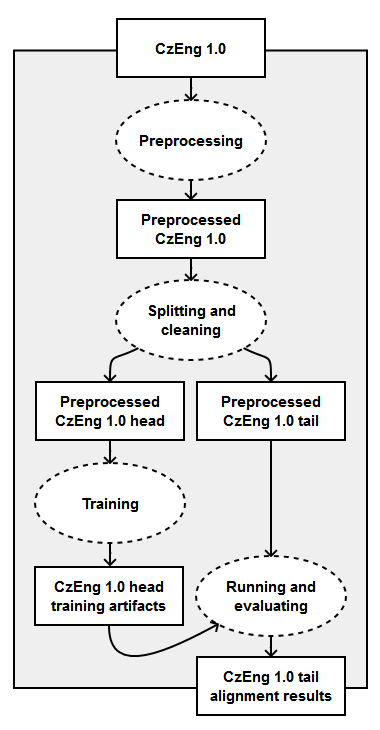
\includegraphics[width=0.50\textwidth]{images/czeng_experiment.png}
\end{figure}

\subsection{Preprocessing CzEng 1.0}
\label{subsection:czeng_experiment_preprocessing}

The entire CzEng 1.0 is preprocessed, as a whole. All the sequences of characters that are neither letters from any alphabet nor whitespaces nor even ASCII symbols are replaced with the Unicode symbol • (U+2022). Then, the corpus is tokenized and subsequently lowercased. The tokenization is done using MorphoDiTa (see Section~\ref{section:morphodita}). When running MorphoDiTa's script \texttt{run\_tokenizer} on the Czech and English parts of the parallel corpus, the argument \texttt{-{}-tokenizer} is set to \texttt{czech} and \texttt{english} respectively.

\subsection{Splitting and Cleaning CzEng 1.0}
\label{subsection:czeng_experiment_cleaning and splitting}

Preprocessed CzEng 1.0 is split horizontally exactly in half creating two separate parallel corpora, i.e.\ head and tail. The head is cleaned by excluding all pairs where either of the two sentences contains more than $50$ tokens ($286,318$ pairs are filtered out) or does not contain a single letter from any alphabet (more $103,251$ are discared). The tail is cleaned by only the latter of the two mentioned filters ($104,103$ pairs are exluded). The pairs containing overly long sentences are removed from the head to get better quality word alignment, which heavily affects the whole training process.

\subsection{Training Part I: Dictionary, Word Vectors}
\label{subsection:czeng_experiment_training_1}

As the first step of the training, SyMGIZA++ is applied (see Section~\ref{subsection:applying_symgiza}) to calculate the word alignment for the head. This includes the standard workflow with the scripts: \texttt{plain2snt}, \texttt{snt2cooc} and \texttt{mkcls}, where we request 2 optimization runs (\texttt{-n2}). For the execution of \texttt{symgiza}, we use the standard settings listed in Table~\ref{table:czeng_symgiza_settings}. From our experience, the method of final symmetrization yielding the best results is the ``union'' method (\texttt{-alig union}).
	
\begin{table}[!htb]
	\centering
	\caption{CzEng experiment: SyMGIZA++ settings}
	\label{table:czeng_symgiza_settings}
	\vspace{1em}
	\begin{tabular}{|l|l|}
		\hline
		\textbf{Description} & \textbf{Argument} \\
		\hline
		Number of threads & \texttt{-ncpus 4} \\
		Number of Model 1 iterations & \texttt{-m1 5} \\
		Number of Model 2 iterations & \texttt{-m2 5} \\
		Number of Model 3 iterations & \texttt{-m3 5} \\
		Number of Model 4 iterations & \texttt{-m4 5} \\
		Number of HMM iterations & \texttt{-mh 5} \\
		Dump Model 1 after 5\textsuperscript{th} iteration & \texttt{-t1} \\
		Dump Model 2 after 5\textsuperscript{th} iteration & \texttt{-t2} \\
		Dump Model 3, 4, 5 after 5\textsuperscript{th} iteration & \texttt{-t345} \\
		Dump Model HMM after 5\textsuperscript{th} iteration & \texttt{-th} \\
		Symmetrize Model 1 after 5\textsuperscript{th} iteration & \texttt{-m1symfrequency 5} \\
		Symmetrize Model 2 after 5\textsuperscript{th} iteration & \texttt{-m2symfrequency 5} \\
		Symmetrize Model 3, 4, 5 after 5\textsuperscript{th} iteration & \texttt{-m345symfrequency 5} \\
		Symmetrize Model HMM after 5\textsuperscript{th} iteration & \texttt{-mhsymfrequency 5} \\
		Symmetrization ``t'' tables multiplier & \texttt{-tm 2} \\
		Run final symmetrization & \texttt{-es 1} \\
		Use Union method in final symmetrization & \texttt{-alig union} \\
		Omit Diagonal option in final symmetrization & \texttt{-diagonal no} \\
		Omit Final option in final symmetrization & \texttt{-final no} \\
		Omit Both option in final symmetrization & \texttt{-both no} \\
		Probability for empty words & \texttt{-emprobforempty 0.0} \\
		Probability smoothing value & \texttt{-probsmooth 1e-7} \\
		\hline
	\end{tabular}
\end{table}

Subsequently, the bilingual dictionary is generated (see Section~\ref{subsection:generating_dictionary}) using the script \texttt{merge\_param.py}. The created dictionary contains $11,567,603$ entries.

Then, bivec is applied (see Section~\ref{subsection:applying_bivec}) to create the bilingual word vectors. Prior to the execution, the training dataset is preprocessed by replacing all the Unicode symbols • (U+2022) symbols with \texttt{<unk>} and the sequences consisting of numbers with zero symbol. We use the standard settings listed in Table~\ref{table:czeng_bivec_settings}. The resulting output contains $367,393$ vectors for the Czech and $179,869$ for the English part of the corpus.
	
\begin{table}[!htb]
	\centering
	\caption{CzEng experiment: bivec settings}
	\label{table:czeng_bivec_settings}
	\vspace{1em}
	\begin{tabular}{|l|l|}
		\hline
		\textbf{Description} & \textbf{Argument}\\
		\hline
		Language code of source language & \texttt{-src-lang en}\\
		Language code of target language & \texttt{-tgt-lang cs}\\
		Use the provided word alignment & \texttt{-align-opt 1}\\
		Cross-lingual learning rate multiplier & \texttt{-bi-weight 1.0}\\
		Use biskip model & \texttt{-cbow 0}\\
		Discard less appearing words & \texttt{-min-count 3}\\
		Size of the output vectors & \texttt{-size 40}\\
		Maximal skip length between words & \texttt{-window 5}\\
		Number of negative examples & \texttt{-negative 5}\\
		Save output in textual format & \texttt{-binary 0}\\
		Do not use hierarchical softmax & \texttt{-hs 0}\\
		Threshold for high-frequency source words & \texttt{-sample 1e-4}\\
		Threshold for high-frequency target words & \texttt{-tgt-sample 1e-4}\\
		Number of threads & \texttt{-threads 4}\\
		Do not evaluate results & \texttt{-eval 0}\\
		Number of iterations & \texttt{-iter 10}\\
		\hline
	\end{tabular}
\end{table}

\subsection{Training Part II: Classifier}
\label{subsection:czeng_experiment_training_2}

The pairs of parallel sentences from the head are distributed into artificial bins to form a supervised dataset for the training of the classifier (see Section~\ref{subsection:preparing_documents}). Each bin contains $50,000$ pairs of the parallel documents, i.e.\ $100,000$ individual documents. We consider this value to be an upper-bound estimate of an average number of paragraphs in either of the two languages located on an ordinary Czech--English web domain. The created dataset consists of $141$ bins. The last bin is an exception containing only $27,110$ pairs.

The document vectors are generated (see Section~\ref{subsection:generating_document_vectors}) using the script \texttt{create\_docvec.py}. The supervised dataset contains $7,027,110$ pairs of the parallel documents for which the script generates $6,467,817$ vectors for the Czech and $6,420,329$ vectors for the English documents. The numbers differ because the script discards duplicated documents within the bins.

The preliminary alignments are created (see Section~\ref{subsection:aligning_document_vectors}) running the script \texttt{align\_docvec.py}. For every Czech document a list of $20$ English candidate documents is created. Annoy (see Section~\ref{section:annoy}) is set to build search indices with $500$ trees and when performing a search it is requested to inspect $500 \times 20 \times 2 = 20,000$ nodes. These settings greatly affect the results. We follow the recommendations~\cite{annoy} to set the number of trees as large as possible given the amount of available memory and the number of nodes to be inspected as large as possible given the amount of available computational time.

The alignments are scored (see Section~\ref{subsection:scoring_alignments}) with the script \texttt{score\_align.py}. In this experiment, we use the expected ratio of the documents's lengths $\mu_{cs \rightarrow en} = 1.08$ with the standard deviation $\sigma_{cs \rightarrow en} = 0.28$. These values were estimated using the pairs of parallel sentences in the head.

The classifier is trained (see Section~\ref{subsection:training_binary_classifier}) with the script \texttt{train\_network.py}. The script creates the training dataset by randomly selecting approximately $20\%$ of all the available pairs of a Czech document with its top English candidate. Additionally, the selection contains nearly as many parallel pairs as non-parallel. The network model is provided by PyBrain (see Section~\ref{section:pybrain}). For completeness, let us describe its configuration; however, we shall not go into details~\cite{Sima96}. The network is a multilayer perceptron learning through the backwards error propagation. It has 4 input, 16 hidden and 2 output neurons. The input neurons are linear, the hidden layer uses sigmoid function and the output layer uses softmax function. The network is trained for $20$ epochs with the $1\%$ learning rate.

\subsection{Running}
\label{subsection:czeng_experiment_running}

The trained system is used to search for sentence pairs in the tail. The pairs of parallel sentences from the tail are distributed into artificial bins in a same manner as those from the head. Also, in this case, each bin contains $50,000$ pairs of the parallel documents, i.e.\ $100,000$ individual documents. In this scenario, each bin simulates a web domain with $50,000$ Czech and $50,000$ English paragraphs that we want to align. In contrast to real websites, these are perfectly parallel, all pages are available in both languages. This way, 147 bins are created. The last bin is an exception containing only $12,576$ pairs. For the purposes of the experiment, the original alignment of the tail is forgotten to not affect anyhow the evaluation process.

For the input dataset, the procedure follows with the exact same steps as for the supervised dataset in the second part of the training. Vectors are generated for all the documents. Using Annoy, the document vectors are aligned into preliminary alignments and these are subsequently scored. All of the settings remain unchanged. The input dataset consists of $7,312,576$ pairs for which $6,750,340$ vectors for the Czech and $6,703,831$ vectors for the English documents are generated. The differences between these numbers are caused again by the presence of duplicate documents within the bins.

In the last step, the trained binary classifier is applied  (see Section~\ref{subsection:applying_binary_classifier}) to obtain the refined alignments for the input dataset. This is done using the script \texttt{apply\_network.py}. The confidence threshold of the classifier is set to $50\%$. The refined alignments represent a subset of all the pairs of Czech documents with their top English candidates that the classifier accepts to be parallel.

\section{Experiment Results}
\label{section:czeng_experiment_results}

With the entire procedure of the experiment described, let us examine the results. The effectiveness of the method is measured after the individual steps of the aligning process. We present the results for the tail from the evaluation but also for the head from the second part of the training. This way we can compare the difference between the results when aligning the data used also in the first part of the training and the data not covered in the training.

Table~\ref{table:czeng_align} shows the quality of the preliminary alignments. The row with an index value $k$ shows how many times the parallel document ends up as a $k\textsuperscript{th}$ best candidate. The one with an index value $k \leq 20$ tells how many times the parallel document appears somewhere in the candidate list and the row with $k > 20$ shows how many times the parallel document is not in a candidate list at all. 

\begin{table}[!htb]
	\centering
	\caption{CzEng experiment: preliminary alignments}
	\label{table:czeng_align}
	\vspace{1em}
	\begin{tabular}{|r||r|r||r|r|}
		\hline
		& \multicolumn{2}{c||}{\textbf{Head (Training)}} & \multicolumn{2}{c|}{\textbf{Tail (Evaluation)}} \\
		\hline
		\textbf{Index} & \textbf{Count} & \textbf{Ratio (\%)} & \textbf{Count} & \textbf{Ratio (\%)} \\ \hline
		1 & 3,310,898 & 51.19 & 3,395,454 & 50.30 \\
		2 & 477,165 & 7.38 & 499,868 & 7.41 \\
		3 & 226,139 & 3.50 & 237,930 & 3.52 \\
		4 & 144,859 & 2.24 & 152,567 & 2.26 \\
		5 & 105,706 & 1.63 & 111,802 & 1.66 \\
		6 & 83,212 & 1.29 & 87,839 & 1.30 \\
		7 & 68,488 & 1.06 & 72,062 & 1.07 \\
		8 & 57,827 & 0.89 & 60,867 & 0.90 \\
		9 & 49,544 & 0.77 & 53,050 & 0.79 \\
		10 & 44,125 & 0.68 & 46,556 & 0.69 \\
		11 & 39,279 & 0.61 & 41,700 & 0.62 \\
		12 & 35,638 & 0.55 & 37,677 & 0.56 \\
		13 & 32,453 & 0.50 & 34,069 & 0.50 \\
		14 & 29,829 & 0.46 & 31,497 & 0.47 \\
		15 & 27,548 & 0.43 & 28,954 & 0.43 \\
		16 & 25,280 & 0.39 & 26,995 & 0.40 \\
		17 & 23,588 & 0.36 & 24,964 & 0.37 \\
		18 & 21,875 & 0.34 & 23,201 & 0.34 \\
		19 & 20,635 & 0.32 & 22,024 & 0.33 \\
		20 & 19,639 & 0.30 & 20,736 & 0.31 \\
		\hline
		$\leq 20$ & 4,843,727 & 74.89 & 5,009,812 & 74.22 \\
		$> 20$ & 1,624,090 & 25.11 & 1,740,528 & 25.78 \\
		\hline
		\textbf{Total} & 6,467,817 & 100.00 & 6,750,340 & 100.00 \\
		\hline
	\end{tabular}
\end{table}

The results for the head show, that $74.89\%$ Czech documents have their parallel English document included in the candidate list. This number is similar also for the tail, where it equals $74.22\%$. The difference is surprisingly small, as the training does not know anything about the tail. By further inspecting the results for the tail, we can observe, that of all the situations when the parallel document appears somewhere in the candidate list, in $67.78\%$ it is the top one and in $94.18\%$ it is included in the top $10$. This means that if we reduce the size of the search from $20$ to $10$, we can still expect approximately $69.89\%$ Czech documents to have the parallel English document somewhere in the candidate list. Reducing the size of the query increases the speed.

Table~\ref{table:czeng_align} shows the quality of the scored alignments. The process of scoring does not change the number of the Czech documents having a parallel English document present in the candidate list. Actually, it only reorders the candidate lists. The intention is to push the parallel documents within their candidate lists to the top as much as possible. The results show that the scoring function based on IBM Model 1 combined with the length comparison is effective. Again, the situation is obviously slightly better for the head. This is mainly caused by the fact, that the bilingual dictionary used in process is built-up from the head only. The results for the tail show that of all the times that parallel document appears in the candidate list, in $96.07\%$ it is the top one. We consider this a good reason why should the following process consider only the top candidates.

\begin{table}[!htb]
	\centering
	\caption{CzEng experiment: scored alignments}
	\label{table:czeng_score}
	\vspace{1em}
	\begin{tabular}{|r||r|r||r|r|}
		\hline
		& \multicolumn{2}{c||}{\textbf{Head (Training)}} & \multicolumn{2}{c|}{\textbf{Tail (Evaluation)}} \\
		\hline
		\textbf{Index} & \textbf{Count} & \textbf{Ratio (\%)} & \textbf{Count} & \textbf{Ratio (\%)} \\ \hline
		1 & 4,689,885 & 72.51 & 4,812,681 & 71.30 \\
		2 & 90,631 & 1.40 & 112,411 & 1.67 \\
		3 & 24,786 & 0.38 & 32,603 & 0.48 \\
		4 & 12,033 & 0.19 & 16,309 & 0.24 \\
		5 & 7,198 & 0.11 & 9,774 & 0.14 \\
		6 & 4,728 & 0.07 & 6,577 & 0.10 \\
		7 & 3,345 & 0.05 & 4,608 & 0.07 \\
		8 & 2,505 & 0.04 & 3,475 & 0.05 \\
		9 & 1,955 & 0.03 & 2,639 & 0.04 \\
		10 & 1,544 & 0.02 & 1,980 & 0.03 \\
		11 & 1,190 & 0.02 & 1,516 & 0.02 \\
		12 & 971 & 0.02 & 1,270 & 0.02 \\
		13 & 746 & 0.01 & 957 & 0.01 \\
		14 & 552 & 0.01 & 781 & 0.01 \\
		15 & 430 & 0.01 & 619 & 0.01 \\
		16 & 407 & 0.01 & 520 & 0.01 \\
		17 & 280 & 0.00 & 407 & 0.01 \\
		18 & 244 & 0.00 & 313 & 0.00 \\
		19 & 179 & 0.00 & 232 & 0.00 \\
		20 & 118 & 0.00 & 140 & 0.00 \\
		\hline
		$\leq 20$ & 4,843,727 & 74.89 & 5,009,812 & 74.22 \\
		$> 20$ & 1,624,090 & 25.11 & 1,740,528 & 25.78 \\
		\hline
		\textbf{Total} & 6,467,817 & 100.00 & 6,750,340 & 100.00 \\
		\hline
	\end{tabular}
\end{table}

The refined alignments are obtained with the $50\%$ confidence threshold. By gradually increasing the threshold and further filtering the alignments we measure the recall and the precision of the classifier at different confidence levels. The results are summarized in Table~\ref{table:czeng_refine}. The first column represents the confidence threshold. The second column represents the number of the document pairs correctly identified to be parallel, i.e.\ the number of true positives. The next column shows the number of false positives, which is the number of document pairs identified as parallel, but in fact they are not. The recall listed in the table is relative to the input of the classification process. The precision is the ratio of the true positives to all the positives. Figure~\ref{figure:czeng_classifier} shows how the recall and the precision change with respect to the confidence threshold of the classifier.

\begin{table}[!htb]
	\centering
	\caption{CzEng experiment: classifier effectiveness}
	\label{table:czeng_refine}
	\vspace{1em}
	\begin{tabular}{|r|r|r|r|r|}
		\hline
		\textbf{Conf.(\%)} & \textbf{True Pos.} & \textbf{False Pos.} & \textbf{Recall (\%)} & \textbf{Precision (\%)} \\ \hline
		50.00 & 4,254,069 & 284,174 & 88.39 & 93.74 \\
		55.00 & 4,179,076 & 248,921 & 86.83 & 94.38 \\
		60.00 & 4,095,812 & 217,081 & 85.10 & 94.97 \\
		65.00 & 4,000,964 & 188,595 & 83.13 & 95.50 \\
		70.00 & 3,892,099 & 162,537 & 80.87 & 95.99 \\
		75.00 & 3,761,728 & 138,619 & 78.16 & 96.45 \\
		80.00 & 3,599,299 & 114,985 & 74.79 & 96.90 \\
		85.00 & 3,385,007 & 89,813 & 70.34 & 97.42 \\
		90.00 & 3,073,706 & 64,730 & 63.87 & 97.94 \\
		95.00 & 2,621,246 & 46,522 & 54.47 & 98.26 \\
		99.00 & 1,808,067 & 23,028 & 37.57 & 98.74 \\
		\hline
	\end{tabular}
\end{table}

\begin{figure}[!htb]
	\centering
	\caption{CzEng experiment: classifier effectiveness}
	\label{figure:czeng_classifier}
	\vspace{1em}
	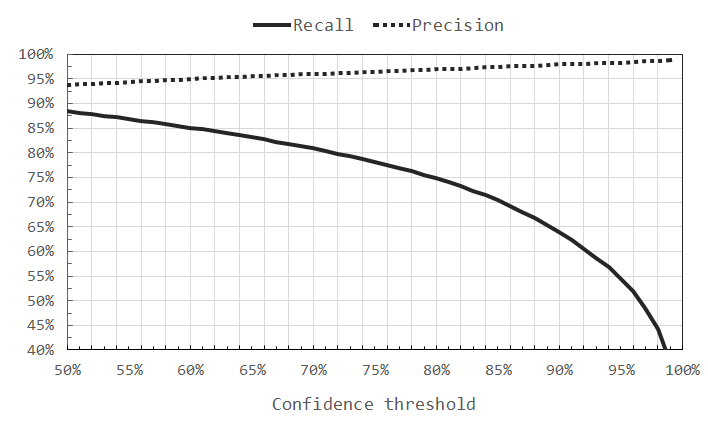
\includegraphics[width=1.00\textwidth]{images/czeng_classifier.png}
\end{figure}

The overall effectiveness of our method is listed in Table~\ref{table:czeng_overall}. These values are measured using the refined alignments without any form of additional filtering.

\begin{table}[!htb]
	\centering
	\caption{CzEng experiment: overall effectiveness}
	\label{table:czeng_overall}
	\vspace{1em}
	\begin{tabular}{|l|r|}
		\hline
		\textbf{Recall (\%)} & 63.02 \\
		\hline
		\textbf{Precision (\%)} & 93.74 \\
		\hline
	\end{tabular}
\end{table}

\section{Experiment Time Duration}
\label{section:czeng_experiment_duration}

The computer used for the experiment execution has Intel\textregistered{} Xeon\textregistered{} CPU E5-2630 v3 (20 MB Cache, 2.40 GHz) and 128 gigabytes (GB) of memory. Table~\ref{table:czeng_time_duration} lists the approximate time durations of the individual steps of the experiment.

\begin{table}[!htb]
	\centering
	\caption{CzEng experiment: time duration}
	\label{table:czeng_time_duration}
	\vspace{1em}
	\begin{tabular}{|l|r|}
		\hline
		\multicolumn{1}{|c|}{\textbf{Activity}} & \multicolumn{1}{c|}{\textbf{Duration (hh:mm)}} \\
		\hhline{|=|=|}
		\multicolumn{2}{|c|}{\textbf{Preprocessing}} \\
		\hline
		Tokenizing and lowercasing & 00:08 \\
		Splitting and cleaning & 00:05 \\
		\hline
		\multicolumn{2}{|c|}{\textbf{Training part I}} \\
		\hline
		Applying SyMGIZA++ & 13:21 \\
		Generating dictionary & 00:10 \\
		Applying bivec & 01:01 \\
		\hline
		\multicolumn{2}{|c|}{\textbf{Training part II}} \\ 
		\hline
		Generating document vectors & 00:37 \\
		Aligning document vectors (Annoy) & 05:52 \\
		Scoring alignments & 02:49 \\
		Training network classifier & 01:29 \\
		\hline
		\multicolumn{2}{|c|}{\textbf{Evaluation}} \\
		\hline
		Generating document vectors & 00:45 \\
		Aligning document vectors (Annoy) & 07:04 \\
		Scoring alignments & 04:10 \\
		Applying network classifier & 00:47 \\
		\hline
	\end{tabular}
\end{table}

\section{Extension: Lemmatization}
\label{section:czeng_experiment_extension}

As already noted (see Section~\ref{subsection:preprocessing_training_parallel_data}), we believe that preprocessing of both training and input data plays an important role in our method. The extension of the experiment described is this section is conducted with a goal to determine whether the lemmatization helps the method to achieve better quality results for the Czech--English language pair.

The procedure of the extended experiment is almost completely the same as in the original experiment. The only difference is in the preprocessing of the data. The lemmatization is added between the tokenization and lowercasing. The lemmatization is done with MorphoDiTa (see Section~\ref{section:morphodita}). When running the script \texttt{run\_tagger} on the Czech and English parts of the parallel corpus, it is provided with the models \texttt{czech-morfflex-pdt-131112.tagger-best\_accuracy}~\cite{Straka13} and \texttt{english-morphium-wsj-140407.tagger}~\cite{Straka14} respectively.

\begin{table}[!htb]
	\centering
	\caption{CzEng experiment (extended): scored alignments}
	\label{table:czeng_extended_score}
	\vspace{1em}
	\begin{tabular}{|r||r|r||r|r|}
		\hline
		& \multicolumn{2}{c||}{\textbf{Head (Training)}} & \multicolumn{2}{c|}{\textbf{Tail (Evaluation)}} \\
		\hline
		\textbf{Index} & \textbf{Count} & \textbf{Ratio (\%)} & \textbf{Count} & \textbf{Ratio (\%)} \\ \hline
		1 & 4,639,484 & 72.10 & 4,813,195 & 71.64 \\
		\vdots & \vdots & \vdots & \vdots & \vdots \\
		\hline
		$\leq 20$ &  4,813,165 & 74.80 & 5,022,948 & 74.76 \\
		$> 20$ & 1,621,610 & 25.20 & 1,695,537 & 25.24 \\
		\hline
		\textbf{Total} & 6,434,775 & 100.00 & 6,718,485 & 100.00 \\
		\hline
	\end{tabular}
\end{table}

With the lemmatization included, the dictionary built-up from the head contains only $6,225,379$ entries ($53.82\%$ of the original size). The extension also reduces the number of word vectors produced by bivec, which is  $173,861$ ($47.32\%$) vectors for the Czech and $163,993$ ($91.17\%$) for the English part of the corpus.

Table~\ref{table:czeng_extended_score} shows how the lemmatization affects the results. It shows the quality of the scored alignments. Although the table is not complete, it contains all the relevant data. The results show minimal improvement. For the tail, the amount of Czech documents having the parallel English document in the candidate list is increased by only $0.54\%$. Additionally, Table~\ref{table:czeng_extended_overall} lists the overall effectiveness of the method with lemmatization included. Again, the results are very similar.

\begin{table}[!htb]
	\centering
	\caption{CzEng experiment (extended): overall effectiveness}
	\label{table:czeng_extended_overall}
	\vspace{1em}
	\begin{tabular}{|l|r|}
		\hline
		\textbf{Recall (\%)} & 63.28 \\
		\hline
		\textbf{Precision (\%)} & 94.32 \\
		\hline
	\end{tabular}
\end{table}

Lemmatization can be thought of as a many-to-one mapping for words. By applying a transformation based on such a mapping we reduce the number of words within a corpus. With less words in the corpus, it is easier for the method to learn the associations between the words; however, the individual sentences are losing their contextual diversity. Apparently, the CzEng 1.0 data are already sufficiently large and the union word alignments do not benefit significantly from the denser statistics due to lemmatization.

%%%%%%%%%%%%%%%%%%%%%%%%%%%%%%%%%%%%%%%%%%%%%%%%%%%%%%%%%%%%%%%%%%%%%%%%%%%%%%%%
%% MASTER'S THESIS                                                            %%
%%                                                                            %% 
%% Title (en): Mining Parallel Corpora from the Web                           %%
%% Title (sk): Rafinácia paralelných korpusov z webu                          %%
%%                                                                            %%
%% Author: Bc. Jakub Kúdela                                                   %%
%% Supervisor: Doc. RNDr. Irena Holubová, Ph.D.                               %%
%% Consultant: RNDr. Ondřej Bojar, Ph.D.                                      %%
%%                                                                            %%
%% Academic year: 2015/2016                                                   %%
%%%%%%%%%%%%%%%%%%%%%%%%%%%%%%%%%%%%%%%%%%%%%%%%%%%%%%%%%%%%%%%%%%%%%%%%%%%%%%%%

\chapter{Web Data (Common Crawl) Experiment}
\label{chapter:web_data_common_crawl_experiment}

In this chapter, the second experiment conducted with our method is discussed. Unlike the first experiment (see Chapter~\ref{chapter:prealigned_data_czeng_experiment}) this one deals with the non-parallel, real-word, noisy data acquired from the web. It illustrates effectiveness of our method in a typical situation for which it is designed.

The selected language pair is the same as in the first experiment, i.e.\ Czech--English. This experiment's procedure utilizes the training artifacts created in the first experiment, namely the dictionary, bilingual word vectors and the trained classifier. The input data are obtained from the July 2015 dataset provided by the Common Crawl organization (see Section~\ref{section:common_crawl}).

The following text describes the procedure of the experiment with an example approach to the task of mining parallel corpus from the Common Crawl dataset for a specific language pair. It also discusses the manually evaluated quality of the acquired Czech--English parallel corpus.

\section{Experiment Procedure}
\label{section:common_crawl_experiment_procedure}

The July 2015 dataset consists of approximately $1.84$ billions of crawled web pages and it takes about $149$ terabytes (TB) of disk space in the uncompressed WARC format. To process this large volume of data we use Hadoop (see Section~\ref{section:hadoop}) cluster provided by MetaCentrum (see Section~\ref{section:metacentrum}). The dataset is available in a form of $33,957$ WARC files compressed by GNU zip (gzip)\footnote{\url{http://www.gzip.org/} (accessed April 23, 2016)}. Each of these files has less than $950$ megabytes (MB) and is accessible via its own URL. The list of these URLs can be obtained at the official website of the Common Crawl~\cite{CommonCrawl} organization. The total size of the July 2015 dataset in the compressed format is approximately $28.5$ TB.

One of the options to get all the files into HDFS (see Subsection~\ref{subsection:hdfs}), is to download them in sequence with cURL\footnote{\url{https://curl.haxx.se/} (accessed April 23, 2016)} using one node of the cluster. During the process, every downloaded file can be immediately copied into HDFS using the command \texttt{hadoop fs -copyFromLocal} and afterwards deleted locally. To reduce the time, the process can use multiple threads. In our environment, we use $5$ threads and the described process takes about $17$ days to complete. Such a long process can be interrupted by many circumstances (e.g.\ cluster maintenance). Therefore, our script first checks which of the files are already present in HDFS using the command \texttt{hadoop fs -ls} to avoid repetitive downloading. Hadoop allows the user to process the WARC files compressed by gzip. We use this feature to reduce the required disk space at the cost of slower execution.

\begin{figure}[!htb]
	\centering
	\caption{Common Crawl experiment}
	\label{figure:common_crawl_experiment}
	\vspace{1em}
	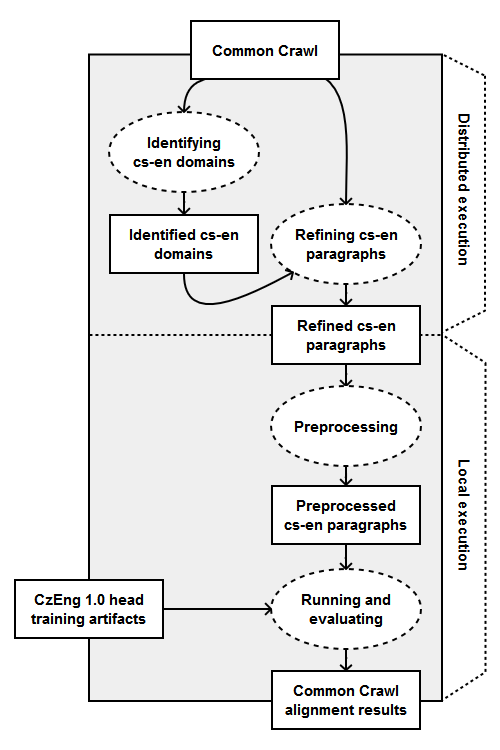
\includegraphics[width=0.65\textwidth]{images/common_crawl_experiment.png}
\end{figure}

With the entire July 2015 dataset stored in HDFS, the experiment illustrated in Figure~\ref{figure:common_crawl_experiment} is applied. The procedure starts with the distributed execution running two MapReduce (see Subsection~\ref{subsection:mapreduce}) jobs. This creates a dataset containing Czech and English paragraphs from the web domains identified to be bilingual. The paragraphs are then aligned with our method in a local execution and the results are evaluated. The whole process is described as follows.

\subsection{Distributed Execution}
\label{subsection:common_crawl_distributed_execution}

The part of the experiment's procedure executed in the distributed environment consists of two MapReduce jobs. The first job identifies the web domains containing paragraphs in both the languages we are interested in. In order to enable the MapReduce framework to read and write the WARC files properly we use WARC-Hadoop (See Section~\ref{section:warc_hadoop}).

Let us describe the implementations of the mapper and the reducer in the first MapReduce job. The mapper is called \textit{WarcTextMapper}. It iterates through the WARC records processing only those which represent HTTP responses with \texttt{text/html} content type, i.e.\ web pages. For every web page it resolves the character encoding and transforms its HTML structure into XHTML using jsoup (see Section~\ref{section:jsoup}). Then, the textual contents of all the \texttt{<p>} HTML tags representing paragraphs are parsed and all those having less than $100$ characters are discarded. The shorter paragraphs are discarded because it is difficult to detect their language reliably. For each paragraph the language is identified with a certain confidence using language-detector (see Section~\ref{section:language_detector}) . The mapper outputs a key-value pair for each paragraph where the language is detected as one of the two languages we are interested in with the confidence at least $99\%$. The structure of an output key-value pair is following:

\vbox{
\begin{itemize}
	\item Key: web domain name.
	\item Value: 
	\begin{enumerate}[label=$\circ$]
		\item language detected by language-detector;
		\item confidence returned by language-detector;
		\item URL associated with the paragraph;
		\item textual content of the paragraph.
	\end{enumerate}
\end{itemize}
}
	
The implementation of the reducer is called \textit{WarcDomainReducer}. For a given web domain (i.e.\ key) it receives the values representing all the paragraphs for the domain emitted by \textit{WarcTextMapper}. The reducer iterates over all these values counting the number of the unique paragraphs (using hashing) and their total length for both the languages separately. It also counts the number of the unique URLs. For every domain having at least one Czech and one English paragraph the reducer outputs the key-value pair as follows:

\vbox{
\begin{itemize}
	\item Key: web domain name.
	\item Value: 
	\begin{itemize}[label=$\circ$]
		\item number of unique URLs;
		\item number of unique English paragraphs;
		\item total length of unique English paragraphs;
		\item number of unique Czech paragraphs;
		\item total length of unique Czech paragraphs.
	\end{itemize}
\end{itemize}
}

The first MapReduce job creates a list of web domains having at least some Czech and English content. Listing~\ref{listing:experiment_domains} shows a sample from its output file. The format contains tab-separated values, where the first column is a web domain, which is the key. The other columns represent the individual items of the value in the order they were listed. The list contains $12,144$ domains. 

\begin{lstlisting}[float=!htb,caption={sample from a file with identified domains},label={listing:experiment_domains},firstnumber=3874]
www.meuslany.cz		2	6	2813	16	4509
www.mff.cuni.cz		7	37	14946	39	18162
\end{lstlisting}

As the next step, a filter is applied on the output of the first MapReduce job reducing the number of web domains to be considered for the further processing. The filter requires from a domain to meet the following condition:
	
\begin{align*}
\frac{\min(N_{cs},N_{en})}{\max(N_{cs},N_{en})} > 1\%,
\end{align*}
	
where $N_{cs}$ and $N_{en}$ are the numbers of Czech and English paragraphs for the domain respectively. The filtering discards all the domains having very unbalanced language distribution. The output contains $8,750$ identified bilingual domains.

The second MapReduce job extracts the Czech and English paragraphs for all the identified bilingual web domains. It uses the same mapper as the first job; however, the implementation of the reducer is different. We call it \textit{WarcTextReducer}. In order to provide the reducer with the file containing the domains Hadoop Distributed Cache is utilized. It is a facility provided by the MapReduce framework enabling the user to cache files for a MapReduce job. Once a file is cached for a job the framework makes it available locally at each node of the cluster for the time of the execution allowing mappers and reducers to read the cached file. When initializing, \textit{WarcTextReducer} reads the entire file with the bilingual domains creating a set of hash codes for all their names. When running, it outputs only those incoming key-value pairs emitted by \textit{WarcTextMapper} that are associated with one of the domains. Additionally, all the values representing duplicate paragraphs are discarded. The structure of the output key-value pairs emitted by both \textit{WarcTextMapper} and \textit{WarcTextReducer} is identical.

Listing~\ref{listing:experiment_paragraphs_cs} and Listing~\ref{listing:experiment_paragraphs_en} show samples of two lines from the output file of the second MapReduce job. These two lines contain parallel paragraphs that are mutual translations. The single output file contains the paragraphs for both the languages. The format is a list of tab-separated values. The first column is a web domain, which is the key. The following columns represent the individual items of the value in the order they were listed in the text describing the structure of the output key-value pairs emitted by \textit{WarcTextMapper}. The output file contains $5,931,091$ paragraphs for both the languages, namely $801,116$ Czech and $5,129,975$ English. The Czech and English paragraphs originate from $127,570$ and $744,074$ unique URLs, respectively. The average length of a Czech paragraph is $352.78$ characters, while for an English one, it is $417.03$.

\begin{lstlisting}[float=!htb,caption={sample from a file with extracted paragraphs (Czech)},label={listing:experiment_paragraphs_cs},firstnumber=3185636]
czechfolks.com	cs	0.99999445885996	http://czechfolks.com/2009/11/25/how-well-do-you-know-the-czech-republic-sweepstakes-results-jak-dobre-znate-ceskou-republiku-a-vysledky-souteze/	Zde je otázka, kterou jsme položili a její správná odpověď: Otázka: Kdo byl Karel IV? Odpověď: Český král a římský císař.
\end{lstlisting}

\begin{lstlisting}[float=!htb,caption={sample from a file with extracted paragraphs (English)},label={listing:experiment_paragraphs_en},firstnumber=3185639]
czechfolks.com	en	0.9999980969126909	http://czechfolks.com/2009/11/25/how-well-do-you-know-the-czech-republic-sweepstakes-results-jak-dobre-znate-ceskou-republiku-a-vysledky-souteze/	Here is the question that we asked with the correct answer: Question: Who was Charles IV? Answer: The king of Bohemia and Holy Roman Emperor.
\end{lstlisting}

\subsection{Local Execution}
\label{subsection:common_crawl_local_execution}

The file containing the extracted paragraphs is transferred from HDFS to a one node of the cluster. The process continues in a single-node execution. The input dataset for our method is formed by distributing the paragraphs into the bins according to domain names. For each bilingual web domain, a bin is created with all the associated paragraphs in both the languages. This restricts the method to align only the paragraphs belonging to the same domain.

The rest of the procedure is similar as for the tail in the first experiment with CzEng 1.0 (see Section~\ref{subsection:czeng_experiment_running}). The input dataset is preprocessed by tokenization and lowercasing and our method is executed creating refined alignments for the paragraphs. The method is provided with the training artifacts created during the first experiment using the head of CzEng 1.0, namely the dictionary, bilingual word vectors and the trained classifier. The only difference in the settings is the changed confidence threshold for the classifier, which is required to be $99\%$. The precision is favoured over the recall. 

It is important to note that for this experiment the Czech language is selected as the source language. Therefore, the paragraph vectors associated with the English language are the ones indexed by Annoy. This selection follows the already mentioned rule of thumb (see Section~\ref{section:method_discussion}) to let the method index the document vectors for the language having more documents.

\section{Experiment Results}
\label{section:common_crawl_experiment_results}

Table~\ref{table:common_crawl_domains} lists the most frequent web domains appearing in the extracted pairs of paragraphs. The full list contains $2,178$ domains having altogether $114,711$ pairs of aligned paragraphs. This means, that the output of our method contains an alignment for $14,32\%$ of all the extracted Czech paragraphs. The extracted paragraph-aligned parallel corpus contains in total $7,235,908$ Czech and $8,369,870$ English tokens.

\begin{table}[!htb]
	\centering
	\caption{Common Crawl experiment: web domains of paragraph pairs}
	\label{table:common_crawl_domains}
	\vspace{1em}
	\begin{tabular}{|l|r|r|}
		\hline
		\textbf{Source Domain} & \textbf{Paragraph Pairs} & \textbf{Ratio (\%)} \\
		\hline
		europa.eu & 23457 & 20.45 \\
		eur-lex.europa.eu & 15037 & 13.11 \\
		windows.microsoft.com & 11905 & 10.38 \\
		www.europarl.europa.eu & 8560 & 7.46 \\
		www.project-syndicate.org & 2210 & 1.93 \\
		www.debian.org & 2191 & 1.91 \\
		support.office.com & 1908 & 1.66 \\
		www.esa.int & 1308 & 1.14 \\
		www.eea.europa.eu & 1299 & 1.13 \\
		www.muni.cz & 1206 & 1.05 \\
		\vdots & \vdots & \vdots  \\
		\hline
		\textbf{Total} & 114,711 & 100.00 \\
		\hline
	\end{tabular}
\end{table}

The quality of the extracted corpus is evaluated manually on a set of randomly selected $500$ paragraph pairs. The inspected pairs are divided into few categories. The results of this subjective evaluation are displayed in Table~\ref{table:common_crawl_refine}. The pair of paragraphs is considered to be a human translation if it seems like created by a human. These are the most favorable ones. If the translation of the pair seems cumbersome, it is labeled as a product of machine translation. The partial match represents a situation when a paragraph is a translation of only a part of the other having some extra content. Everything else is labeled as a mismatch.

\begin{table}[!htb]
	\centering
	\caption{Common Crawl experiment: evaluation (500 paragraph pairs)}
	\label{table:common_crawl_refine}
	\vspace{1em}
	\begin{tabular}{|l|r|r|}
		\hline
		\textbf{Category} & \textbf{Count} & \textbf{Ratio (\%)} \\
		\hline
		Human translation & 466 & 93.20 \\
		Machine translation & 7 & 1.40 \\
		Partial match & 13 & 2.60 \\
		Mismatch & 14 & 2.80 \\
		\hline
		\textbf{Total} & 500 & 100.00 \\
		\hline
	\end{tabular}
\end{table}

To estimate the precision of our method, let us consider the pairs of paragraphs belonging to the categories of human and machine translation as the true positives. This way all the other pairs are regarded as the false positives. Table~\ref{table:common_crawl_precision} shows how the precision of the method changes with respect to the confidence threshold of the classifier.

\begin{table}[!htb]
	\centering
	\caption{Common Crawl experiment: precision (500 paragraph pairs)}
	\label{table:common_crawl_precision}
	\vspace{1em}
	\begin{tabular}{|r|r|r|r|}
		\hline
		\textbf{Conf.(\%)} & \textbf{True Pos.} & \textbf{False Pos.} & \textbf{Precision (\%)} \\ \hline
		99.00 & 473 & 27 & 94.60 \\
		99.10 & 464 & 25 & 94.89 \\
		99.20 & 456 & 23 & 95.20 \\
		99.30 & 446 & 20 & 95.71 \\
		99.40 & 435 & 17 & 96.24 \\
		99.50 & 415 & 16 & 96.29 \\
		99.60 & 404 & 16 & 96.19 \\
		99.70 & 386 & 12 & 96.98 \\
		99.80 & 357 & 7 & 98.08 \\
		99.90 & 286 & 3 & 98.96 \\
		\hline
	\end{tabular}
\end{table}

The task of estimating the recall of our method is more difficult. We would need to manually inspect all the paragraphs from every web domain selected for the evaluation. Therefore, let us perform the recall estimation for only one web domain with smaller number of paragraphs present in the input dataset. The selected web domain is \texttt{www.csa.cz}, the official website of Czech Airlines containing human-translated content. For the domain, the input dataset contains $68$ Czech and $87$ English paragraphs. These are manually aligned, creating what we consider to be the ideal alignments. When evaluated, the ideal alignments contain $44$ paragraph pairs, of which $42$ appear also in the corpus extracted by our method. Additionally, the corpus include $1$ extra pair subjectively regarded as mismatch. Table~\ref{table:common_crawl_effectiveness} shows the effectiveness of our method evaluated for the \texttt{www.csa.cz} web domain. The results are satisfactory; however, \texttt{www.csa.cz} is a website with a large proportion of the content provided in both the languages. This fact makes it one of the cleaner sources of parallel Czech--English content.

\begin{table}[!htb]
	\centering
	\caption{Common Crawl experiment: effectiveness (\texttt{www.csa.cz})}
	\label{table:common_crawl_effectiveness}
	\vspace{1em}
	\begin{tabular}{|l|r|}
		\hline
		\textbf{Recall (\%)} & 95.45 \\
		\hline
		\textbf{Precision (\%)} & 97.67 \\
		\hline
	\end{tabular}
	\vspace{2em} 
\end{table}

\section{Experiment Time Duration}
\label{section:common_crawl_experiment_duration}

The cluster used for the distributed execution of the MapReduce jobs is described in Section~\ref{section:metacentrum}. The rest of the procedure, i.e.\ the local execution, is done on one node of the cluster having Intel\textregistered{} Xeon\textregistered{} CPU E5-2630 v3 (20 MB Cache, 2.40 GHz) and 128 gigabytes (GB) of memory. Table~\ref{table:common_crawl_time_duration} contains the approximate time durations of the individual steps of the experiment.

\begin{table}[!htb]
	\centering
	\caption{Common Crawl experiment: time duration}
	\label{table:common_crawl_time_duration}
	\vspace{1em}
	\begin{tabular}{|l|r|}
		\hline
		\multicolumn{1}{|c|}{\textbf{Activity}} & \multicolumn{1}{c|}{\textbf{Duration (hh:mm)}} \\
		\hhline{|=|=|}
		\multicolumn{2}{|c|}{\textbf{MapReduce framework}} \\
		\hline
		Identifying cs-en domains & 11:58 \\
		Refining cs-en paragraphs & 11:38 \\
		\hline
		\multicolumn{2}{|c|}{\textbf{Local Execution}} \\
		\hline
		Tokenization and lowercasing & 00:09 \\
		Generating document vectors & 00:58 \\
		Aligning document vectors (Annoy) & 01:13 \\
		Scoring alignments & 03:42 \\
		Applying network classifier & 00:39 \\
		\hline
	\end{tabular}
\end{table}

%%%%%%%%%%%%%%%%%%%%%%%%%%%%%%%%%%%%%%%%%%%%%%%%%%%%%%%%%%%%%%%%%%%%%%%%%%%%%%%%
%% MASTER'S THESIS                                                            %%
%%                                                                            %% 
%% Title (en): Mining Parallel Corpora from the Web                           %%
%% Title (sk): Rafinácia paralelných korpusov z webu                          %%
%%                                                                            %%
%% Author: Bc. Jakub Kúdela                                                   %%
%% Supervisor: Doc. RNDr. Irena Holubová, Ph.D.                               %%
%% Consultant: RNDr. Ondřej Bojar, Ph.D.                                      %%
%%                                                                            %%
%% Academic year: 2015/2016                                                   %%
%%%%%%%%%%%%%%%%%%%%%%%%%%%%%%%%%%%%%%%%%%%%%%%%%%%%%%%%%%%%%%%%%%%%%%%%%%%%%%%%

\chapwithtoc{Conclusions and Future Work}

The main objectives of our thesis were to propose a new method for bilingual document alignment, applicable in the field of mining parallel data from the web, and to conduct experiments with the method, presenting its capabilities and effectiveness. The method is partially inspired by the related work, but it is based on a different approach.

The majority of the known methods search for pairs of parallel web pages by the similarity of their HTML structures. They also rely on HTML structures when aligning contents of web pages already identified as parallel. In contrast to these methods, our method does not depend on any kind of page structure comparison at all. 

The proposed method is supervised and generic in nature. First, it needs to be trained using a provided sentence-aligned parallel corpus for a given language pair. When trained, the method solves the task of bilingual document alignment---given a set of documents in the two languages, it finds the pairs of parallel ones. With the method applied to the task of mining parallel corpora from the web, we are able to effectively identify the pairs of parallel segments (i.e.\ paragraphs) located anywhere on the pages of a web domain, regardless of their structure. 

The most important step of our method is based on the combination of recent ideas, namely the bilingual extension of word2vec---bivec---and the locality-sensitive hashing (LSH). The method uses bivec to learn vectors for the words in both languages from a provided training parallel corpus. The word vectors are used to calculate the aggregate vectors for the documents to be aligned. These document vectors belong to a common vector space, where pairs of parallel documents tend to have similar vectors. To effectively search the space of document vectors for parallel document candidates, we use Annoy---an implementation of the approximate-nearest-neighbours search based on SimHash, one of the LSH algorithms. In order to decide whether to accept a pair of document and its candidate as parallel or not, a binary classifier is trained using the provided training parallel corpus. The classifier model is based on a neural network, and it uses a set of defined features for the classification.

\section*{Results}

To verify the idea of our method, we have performed two experiments focused on the Czech--English language pair. The first one uses prealigned data, and its results are evaluated automatically. It simulates a scenario with $147$ web domains, each of them containing approximately $50,000$ Czech and $50,000$ English paragraphs to be aligned. In the experiment, the ideal solution consists of an alignment for each paragraph. The results of the experiment are $63.28\%$ recall at $94.32\%$ precision. In an extension of the experiment, we have observed that including lemmatization into the standard preprocessing (tokenization and lowercasing) of both the training and input data does not improve the quality of the resulting alignments notably.

The second experiment involves the real-world data provided by the Common Crawl Foundation. It demonstrates an application of our method to mining parallel corpora from a hundreds of terabytes (TB) large set of web-crawled data. We have managed to extract the Czech--English parallel corpus from a 149 TB large dataset consisting of 1.84 billions of web pages. By implementing and running two MapReduce jobs, we were able to identify $8,750$ web domains having detectable amount of Czech--English bilingual content, and we have managed to extract $801,116$ Czech and $5,931,091$ English paragraphs from these domains. The extracted paragraphs were aligned with our method, creating a paragraph-aligned parallel corpus containing $114,771$ pairs from $2,178$ domains, having in total $7,235,908$ Czech and $8,369,870$ English tokens. The quality of the acquired corpus has been evaluated manually on a set of $500$ randomly selected pairs. The precision was estimated to be $94,60\%$. To evaluate the recall, we have selected one web domain (\texttt{www.csa.cz}) with a smaller number of paragraphs present in the input dataset. The results for the domain were estimated to be $95.45\%$ recall at $97.67\%$ precision.

We were surprised by the size of the corpus created in the second experiment, as we have expected to extract larger quantities of parallel paragraphs. However, we are convinced that the size is not affected that much by inferior recall of our approach, but the fact that the dataset does not contain many Czech--English web pages. The size of the corpus is comparable with the amount of Czech--English parallel data acquired by the previous project, focused on mining the Common Crawl datasets described in the related work~\cite{Smith13}. Additionally, our approach achieves a higher precision. 

The datasets produced by Common Crawl usually contain only a small subset of all the pages available on a web domain at the crawling time. Therefore, the approach described in the second experiment could be extended. We could use the list of web domains with identified Czech--English content to run our own targeted crawling that would navigate through the pages in more depth.

\section*{Future Work}

Both experiments show satisfactory results, implying that the proposed method is a promising baseline for acquiring parallel corpora from the web. Nevertheless, there is still some room for improvement.
First of all, our method does not consider word order in the aligning process at any stage. Both the scoring function and the features designed for the classification could be extended to take this aspect into account.

Then there is the asymmetric nature of our method, meaning it generates different results if the source and the target languages are swapped. It could be extended to run the alignment for both directions and the results could be symmetrized. This might help the method achieve an even higher precision.

Finally, we have run our method only in a single-node environment so far. This is largely because we were aligning a relatively small sets of documents (not more than $15,000,000$).
However, the method is designed to run in distributed fashion. Bins with input documents represent independent isolable tasks. Once the method is trained, these tasks could be distributed across multiple cluster nodes together with the resources needed for the aligning process. This would increase the throughput of our method and hence decrease the execution time.

%%%%%%%%%%%%%%%%%%%%%%%%%%%%%%%%%%%%%%%%%%%%%%%%%%%%%%%%%%%%%%%%%%%%%%%%%%%%%%%%
%% MASTER'S THESIS                                                            %%
%%                                                                            %% 
%% Title (en): Mining Parallel Corpora from the Web                           %%
%% Title (sk): Rafinácia paralelných korpusov z webu                          %%
%%                                                                            %%
%% Author: Bc. Jakub Kúdela                                                   %%
%% Supervisor: Doc. RNDr. Irena Holubová, Ph.D.                               %%
%% Consultant: RNDr. Ondřej Bojar, Ph.D.                                      %%
%%                                                                            %%
%% Academic year: 2015/2016                                                   %%
%%%%%%%%%%%%%%%%%%%%%%%%%%%%%%%%%%%%%%%%%%%%%%%%%%%%%%%%%%%%%%%%%%%%%%%%%%%%%%%%

\addcontentsline{toc}{chapter}{Bibliography}
\begin{thebibliography}{99}

% Book
\bibitem{Koehn09}
Philipp Koehn
\textit{Statistical Machine Translation},
Cambridge University Press, 2009

% Conference paper
\bibitem{Tiedemann12}
Jörg Tiedemann,
'Parallel Data, Tools and Interfaces in OPUS'
in \textit{Proceedings of the 8\textsuperscript{th} International Conference on Language Resources and Evaluation (LREC'12)},
pages 2214--2218,
European Language Resources Association (ELRA), 2012 

% Journal article
\bibitem{Mikolov13a}
Tomas Mikolov, Kai Chen, Greg Corrado, Jeffrey Dean
'Efficient Estimation of Word Representations in Vector Space'
in \textit{In Proceedings of Workshop at ICLR},
2013,
\url{http://arxiv.org/abs/1301.3781} (accessed April 6, 2016)

% Journal article
\bibitem{Mikolov13b}
Tomas Mikolov, Quoc V. Le, Ilya Sutskever
'Exploiting Similarities among Languages for Machine Translation'
in \textit{Computing Research Repository, arXiv},
2013,
\url{http://arxiv.org/abs/1309.4168} (accessed April 6, 2016)

% Journal article
\bibitem{Mikolov13c}
Tomas Mikolov, Ilya Sutskever, Kai Chen, Greg Corrado, Jeffrey Dean
'Distributed Representations of Words and Phrases and their Compositionality'
in \textit{Computing Research Repository, arXiv},
2013,
\url{http://arxiv.org/abs/1310.4546} (accessed April 6, 2016)

% Journal article
\bibitem{Charikar02}
Moses S. Charikar
'Similarity estimation techniques from rounding algorithms'
in \textit{Proceedings of the 34\textsuperscript{th} Annual ACM Symposium on Theory of Computing},
pages 380--388,
ACM New York, NY, USA,
2002

% Journal article
\bibitem{Andoni08}
Alexandr Andoni, Piotr Indyk
'Near-optimal hashing algorithms for approximate nearest neighbor in high dimensions'
in \textit{Near-optimal Hashing Algorithms for Approximate Nearest Neighbor in High Dimensions},
pages 117--122,
ACM New York, NY, USA,
2002

% Journal article
\bibitem{Tiedemann11}
Jörg Tiedemann,
'Bitext alignment'
in \textit{Synthesis Lectures on Human Language Technologies},
pages 1--165,
Morgan \& Claypool Publishers, 2011

% Book
\bibitem{Bojar12_1}
Ondřej Bojar
'Čeština a strojový překlad: Strojový překlad našincům, našinci strojovému překladu',
Institute of Formal and Applied Linguistics, 
Charles University in Prague, Czech Republic, 
Faculty of Mathematics and Physics,
2015

% Conference paper
\bibitem{Bojar12_2}
Ondřej Bojar, Zdeněk Žabokrtský, Ondřej Dušek, Petra Galuščáková, Martin Majliš, David Mareček, Jiří Maršík, Michal Novák, Martin Popel, Aleš Tamchyna
'The joy of parallelism with CzEng 1.0'
in \textit{Proceedings of the 8\textsuperscript{th} International Conference on Language Resources and Evaluation (LREC'12)},
European Language Resources Association (ELRA), 2012

% Conference paper
\bibitem{CommonCrawl}
Common Crawl Foundation
'Common Crawl'
\url{http://commoncrawl.org/} (accessed March 19, 2016)

% Journal article
\bibitem{EsplaGomis09}
Miquel Esplà-Gomis, Mikel L. Forcada
'Bitextor, a free/open-source software to harvest translation memories from multilingual websites'
in \textit{Proceedings of the workshop {B}eyond {T}ranslation {M}emories: New Tools for Translators {MT}},
Association for Machine Translation in the Americas, 2009

% Journal article
\bibitem{EsplaGomis10}
Miquel Esplà-Gomis, Mikel L. Forcada
'Combining Content-Based and URL-Based Heuristics to Harvest Aligned Bitexts from Multilingual Sites with Bitextor'
in \textit{The Prague Bulletin of Mathematical Linguistics},
volume 93,
pages 77--86,
2010

% Web resource
\bibitem{HTML}
Ian Hickson, Robin Berjon, Steve Faulkner, Travis Leithead, Erika Doyle Navara, Edward O'Connor, Silvia Pfeiffer
'HTML5 -- A vocabulary and associated APIs for HTML and XHTML',
October 2014,
\url{http://www.w3.org/TR/2014/REC-html5-20141028/} (accessed March 27, 2016)

% Web resource
\bibitem{XML}
Tim Bray, Jean Paoli, C. M. Sperberg-McQueen, Eve Maler, François Yergeau
'Extensible Markup Language (XML) 1.0 (5\textsuperscript{th} Edition)', 
November 2008,
\url{https://www.w3.org/TR/2006/REC-xml-20060816/} (accessed March 27, 2016)

% Web resource
\bibitem{TMX}
Yves Savourel
'TMX 1.4b Specification',
June 2011,
\url{https://www.gala-global.org/tmx-14b} (accessed March 27, 2016)

% Web resource
\bibitem{XHTML}
Steven Pemberton et. al.
'XHTML\textsuperscript{TM} 1.0 The Extensible HyperText Markup Language (2\textsuperscript{nd} Edition)'
January 2000,
\url{https://www.w3.org/TR/2002/REC-xhtml1-20020801} (accessed March 27, 2016)

% Journal article
\bibitem{Lui12}
Marco Lui, 	Timothy Baldwin
'langid.py: an off-the-shelf language identification tool'
in \textit{Proceedings of the ACL 2012 System Demonstrations},
pages 25--30,
2012

% Journal article
\bibitem{Brown93}
Peter F. Brown, Vincent J. Della Pietra, Stephen A. Della Pietra, Robert L. Mercer
'The mathematics of statistical machine translation: parameter estimation'
in \textit{Computational Linguistics - Special issue on using large corpora: II},
volume 19, issue 2, June 1993 
pages 263--311,
MIT Press Cambridge, MA, USA, 1993

% Journal article
\bibitem{Varga05}
Dániel Varga, László Németh, Péter Halácsy, András Kornai, Viktor Trón, Viktor Nagy
'Parallel corpora for medium density languages'
in \textit{In Proceedings of the RANLP 2005},
pages 590--596,
2005

% Journal article
\bibitem{Gale93}
William A. Gale, Kenneth W. Church
'A program for aligning sentences in bilingual corpora'
in \textit{Computational Linguistics - Special issue on using large corpora: I},
volume 19, issue 1, March 1993,
pages 75--102,
MIT Press Cambridge, MA, USA, 1993

% Journal article
\bibitem{Vincente12}
Iñaki San Vicente, Iker Manterola
'PaCo2: A Fully Automated tool for gathering Parallel Corpora from the Web'
in \textit{Proceedings of the 8\textsuperscript{th} International Conference on Language Resources and Evaluation (LREC'12)},
European Language Resources Association (ELRA), 2012

% Journal article
\bibitem{Resnik03}
Philip Resnik, Noah A. Smith
'The Web as a parallel corpus'
in \textit{Computational Linguistics - Special issue on web as corpus},
volume 29, issue 3, September 2003,
pages 349--380,
MIT Press Cambridge, MA, USA, 2003

% Journal article
\bibitem{Nadeau04}
David Nadeau, George Foster
'Real-time identification of parallel texts from bilingual newsfeed'
in \textit{CLINE 2004, Computational Linguistics in the North East},
2004

% Journal article
\bibitem{Ratcliff88}
John W. Ratcliff, David Metzener
'Pattern Matching: The Gestalt Approach'
in \textit{Dr. Dobb's Journal},
volume 7,
page 46,
1988

% Journal article
\bibitem{Resnik99}
Philip Resnik
'Mining the Web for Bilingual Text'
in \textit{Proceedings of the 37\textsuperscript{th} annual meeting of the Association for Computational Linguistics (ACL)},
pages 527--534,
University of Maryland, College Park, Maryland, 1999

% Journal article
\bibitem{Resnik98}
Philip Resnik
'Parallel Strands: A Preliminary Investigation into Mining the Web for Bilingual Text',
in \textit{In 3\textsuperscript{rd} Conference of the Association for Machine Translation in the Americas},
pages 72--82,
Springer, 
1998

% Journal article
\bibitem{Hunt75}
James W. Hunt, Malcolm D. McIlroy
'An Algorithm for Differential File Comparison'
in \textit{Technical Memorandum 75-1271-11},
Bell Laboratories, 
1975

% Journal article
\bibitem{Pearson95}
Karl Pearson
'Notes on regression and inheritance in the case of two parents'
in \textit{Proceedings of the Royal Society of London},
volume 58,
pages 240--242,
1895

% Journal article
\bibitem{Wolk14}
Krzysztof Wołk, Krzysztof Marasek
'Building subject-aligned comparable corpora and mining it for truly parallel sentence pairs'
in \textit{Procedia Technology},
volume 18,
pages 126--132,
International workshop on Innovations in Information and Communication Science and Technology (IICST),
2014

% Journal article
\bibitem{Miller95}
George A. Miller
'WordNet: A Lexical Database for English'
in \textit{Communications of the ACM},
volume 38,
pages 39--41,
1995

% Journal article
\bibitem{Fellbaum98}
Christiane Fellbaum
'WordNet: An Electronic Lexical Database',
MIT Press, 
1998

% Journal article
\bibitem{Loper02}
Edward Loper, Steven Bird
'NLTK: The Natural Language Toolkit'
in \textit{Proceedings of the ACL 2012 Workshop on Effective Tools and Methodologies for Teaching Natural Language Processing and Computational Linguistics},
volume 1,
pages 63--70,
2002

% Journal article
\bibitem{Koehn07}
Philipp Koehn, Hieu Hoang, Alexandra Birch, Chris Callison-Burch, Marcello Federico, Nicola Bertoldi, Brooke Cowan, Wade Shen, Christine Moran, Richard Zens, Chris Dyer, Ondřej Bojar, Alexandra Constantin, Evan Herbst	
'Moses: open source toolkit for statistical machine translation'
in \textit{Proceedings of the ACL 2012 Workshop on Effective Tools and Methodologies for Teaching Natural Language Processing and Computational Linguistics},
volume 1,
pages 63--70,
2002

% Web resource
\bibitem{Moses}
Philipp Koehn
'MOSES User Manual and Code Guide'
2016,
\url{http://www.statmt.org/moses/manual/manual.pdf} (accessed April 5, 2016)

% Journal article
\bibitem{Smith13}
Jason R. Smith, Herve Saint-Amand, Magdalena Plamada, Philipp Koehn, Chris Callison-Burch, Adam Lopez
'Dirt Cheap Web-Scale Parallel Text from the Common Crawl'
in \textit{Proceedings of the 37\textsuperscript{th} annual meeting of the Association for Computational Linguistics (ACL) on Interactive Poster and Demonstration Sessions},
Pages 177--180 ,
Association for Computational Linguistics,
2007

% Journal article
\bibitem{Dean04}
Jeffrey Dean, Sanjay Ghemawat
'MapReduce: simplified data processing on large clusters'
in \textit{Proceedings of the 6\textsuperscript{th} Conference on Symposium on Opearting Systems Design \& Implementation}
volume 6,
pages 137--149,
USENIX Association,
2004

% Journal article
\bibitem{Burch11}
Chris Callison-Burch, Philipp Koehn, Christof Monz, Omar F. Zaidan
'Findings of the 2011 workshop on statistical machine translation'
in \textit{Proceedings of the 6\textsuperscript{th} Workshop on Statistical Machine Translation},
pages 22--64,
Association for Computational Linguistics,
2011

% Book
\bibitem{Holubova15}
Holubová Irena, Kosek Jiří, Minařík Karel, Novák David
'Big Data a NoSQL databáze',
Grada Publishing, a.s., 
2015

% Conference paper
\bibitem{Strakova14}
Straková Jana, Straka Milan and Hajič Jan
'Open-Source Tools for Morphology, Lemmatization, POS Tagging and Named Entity Recognition'
in \textit{Proceedings of 52\textsuperscript{nd} Annual Meeting of the Association for Computational Linguistics: System Demonstrations},
pages 13--18,
Association for Computational Linguistics,
2014

% Conference paper
\bibitem{Spoustova09}
Drahomíra Spoustová, Jan Hajič, Jan Raab, Miroslav Spousta
'Semi-Supervised Training for the Averaged Perceptron POS Tagger'
in \textit{Proceedings of the 12th Conference of the European Chapter of the ACL (EACL 2009)},
pages 763--771,
Association for Computational Linguistics,
2009

% Web resource
\bibitem{Straka13}
Straka Milan, Straková Jana
'Czech Models (MorfFlex CZ + PDT) for MorphoDiTa',
2013,
LINDAT/CLARIN digital library at Institute of Formal and Applied Linguistics, Charles University in Prague,
\url{http://hdl.handle.net/11858/00-097C-0000-0023-68D8-1} (accessed April 7, 2016)

% Web resource
\bibitem{Straka14}
Straka Milan, Straková Jana
'English Models (Morphium + WSJ) for MorphoDiTa',
LINDAT/CLARIN digital library at Institute of Formal and Applied Linguistics, Charles University in Prague,
2014,
\url{http://hdl.handle.net/11858/00-097C-0000-0023-68D9-0} (accessed April 7, 2016)


% Conference paper
\bibitem{Junczys10}
Marcin Junczys-Dowmunt, Arkadiusz Szał
'SyMGiza++: A Tool for Parallel Computation of Symmetrized Word Alignment Models'
in \textit{Proceedings of the 5\textsuperscript{th} International Multiconference on Computer Science and Information Technology},
pages 397--401,
2010

% Conference paper
\bibitem{Vogel96}
'HMM-based word alignment in statistical translation'
in \textit{Proceedings of the 16\textsuperscript{th} conference on Computational linguistics - Volume 2},
pages 836--841,
Association for Computational Linguistics,
1996

% Journal article
\bibitem{Och03}
Franz Josef Och, Hermann Ney
'A systematic comparison of various statistical alignment models'
in \textit{Computational Linguistics},
volume 29, number 1,
pages 19--51,
2003

% Journal article
\bibitem{Dempster77}
Arthur P. Dempster, Nan M. Laird, and Donald B. Rubin
'Maximum Likelihood from Incomplete Data via the EM Algorithm'
in \textit{Journal of the Royal Statistcial Society},
series B, volume 39, number 1,
pages 1--38,
1977

% Conference paper
\bibitem{Och99}
Franz Josef Och
'An Efficient Method for Determining Bilingual Word Classes'
in \textit{Proceeding EACL '99 Proceedings of the 9\textsuperscript{th} conference on European chapter of the Association for Computational Linguistics},
pages 71--76,
Association for Computational Linguistics,
1999

% Conference paper
\bibitem{Gao08}
Qin Gao, Stephan Vogel
'Parallel implementations of word alignment tool'
in \textit{SETQA-NLP '08 Software Engineering, Testing, and Quality Assurance for Natural Language Processing}
pages 49--57,
2008

% Conference paper
\bibitem{Dyer13}
Chris Dyer, Victor Chahuneau and Noah A. Smith
'A simple, fast, and effective reparameterization of IBM model 2'
in \textit{Proceedings of NAACL-HLT 2013},
pages 644--648,
2013

% Journal article
\bibitem{Luong15}
Minh-Thang Luong, Hieu Pham, and Christopher D. Manning
'Bilingual Word Representations with Monolingual Quality in Mind'
in \textit{Proceedings of the 1\textsuperscript{st} Workshop on Vector Space Modeling	for Natural Language Processing},
pages 151-–159,
2015

% Journal article
\bibitem{Rong14}
Xin Rong
'word2vec Parameter Learning Explained'
in \textit{Computing Research Repository, arXiv}
2014,
\url{http://arxiv.org/abs/1411.2738} (accessed April 6, 2016)

% Journal article
\bibitem{Pennigton14}
Jeffrey Pennington, Richard Socher, Christopher D. Manning
'GloVe: Global Vectors for Word Representation'
in \textit{Proceedings of the 2014 Conference on Empirical Methods in Natural Language Processing (EMNLP)},
pages 1532--1543,
Association for Computational Linguistics,
2014

% Jornal article
\bibitem{Gouws14}
Stephan Gouws, Yoshua Bengio, Greg Corrado
'BilBOWA: Fast Bilingual Distributed Representations without Word Alignments'
in \textit{Computing Research Repository, arXiv}
2014,
\url{http://arxiv.org/abs/1410.2455} (accessed April 7, 2016)

% Web resource
\bibitem{annoy}
Erik Bernhardsson et al.
'Annoy: Approximate Nearest Neighbors in C++/Python',
2016,
\url{https://github.com/spotify/annoy} (accessed April 11, 2016)

% Web resource
\bibitem{Bernhardsson16}
Erik Bernhardsson et al.
'Benchmarks of approximate nearest neighbor libraries in Python',
2016,
\url{https://github.com/erikbern/ann-benchmarks} (accessed April 11, 2016)

% Journal article
\bibitem{Schaul10}
Tom Schaul, Justin Bayer, Daan Wierstra, Yi Sun, Martin Felder, Frank Sehnke, Thomas Rückstieß, Jürgen Schmidhuber
'PyBrain'
in \textit{The Journal of Machine Learning Research},
volume 11,
pages 743--746,
2010

% Book
\bibitem{Sima96}
Jiri Sima, Roman Neruda
'Theoretical Issues of Neural Networks',
MatfyzPress, Prague, 
1996

% Journal article
\bibitem{Rumelhart86}
David E. Rumelhart, Geoffrey E. Hinton, Ronald J.Williams
'Learning internal representations by error propagation',
in \textit{Parallel distributed processing: explorations in the microstructure of cognition},
volume 1,
pages 348--362,
MIT Press, Cambridge MA,
1986

% Web resource
\bibitem{WARC}
'ISO 28500:2009 - Information and documentation -- WARC file format',
International Organization for Standardization, Geneva, Switzerland.
2009,
\url{http://www.iso.org/iso/catalogue_detail.htm?csnumber=44717} (accessed April 8, 2016)

% Web resource
\bibitem{JSON}
Timothy W. Bray
'The JavaScript Object Notation (JSON) Data Interchange Format',
March 2014,
\url{https://tools.ietf.org/html/rfc7159} (accessed April 18, 2016)

% Book
\bibitem{White15}
Tom White
'Hadoop: The Definitive Guide, 4\textsuperscript{th} Edition',
O'Reilly Media,
2015

% Book
\bibitem{Gosling14}
James Gosling, Bill Joy, Guy L. Steele, Gilad Bracha, Alex Buckley
'The Java Language Specification, Java SE 8 Edition',
Addison-Wesley Professional,
2014

% Book
\bibitem{Lindholm14}
Tim Lindholm, Frank Yellin, Gilad Bracha, Alex Buckley
'The Java Virtual Machine Specification, Java SE 8 Edition',
Addison-Wesley Professional,
2014

% Journal article
\bibitem{Ghemawat03}
Sanjay Ghemawat, Howard Gobioff, Shun-Tak Leung
'The Google File System'
in \textit{Proceedings of the 19\textsuperscript{th} ACM Symposium on Operating Systems Principles},
pages 29--43,
ACM New York, NY, USA,
2003,

% Journal article
\bibitem{Shvachko10}
Konstantin Shvachko, Hairong Kuang, Sanjay Radia, Robert Chansler
'The Hadoop Distributed File System'
in \textit{Proceedings of the 2010 IEEE 26\textsuperscript{th} Symposium on Mass Storage Systems and Technologies (MSST)},
pages 1--10,
2010,
IEEE Computer Society

% Web resource
\bibitem{hdfs_architecture}
Apache Software Foundation
'HDFS Architecture',
2016
\url{https://hadoop.apache.org/docs/r2.7.2/hadoop-project-dist/hadoop-hdfs/HdfsDesign.html} (accessed April 18, 2016),

% Web resource
\bibitem{mapreduce_tutorial}
Apache Software Foundation
'MapReduce Tutorial',
2016
\url{https://hadoop.apache.org/docs/r2.7.2/hadoop-mapreduce-client/hadoop-mapreduce-client-core/MapReduceTutorial.html} (accessed April 22, 2016),

% Web resource
\bibitem{warc-hadoop}
Martin Kleppmann
'warc-hadoop: WARC Input and Output Formats for Hadoop',
2014,
\url{https://github.com/ept/warc-hadoop} (accessed April 10, 2016),

% Web resource
\bibitem{jsoup}
Jonathan Hedley et al.
'jsoup: Java HTML parser',
2015,
\url{https://jsoup.org/} (accessed April 10, 2016),

% Web resource
\bibitem{DOM}
Anne van Kesteren, Aryeh Gregor, Ms2ger, Alex Russell, Robin Berjon
'W3C DOM4', 
November 2015,
\url{https://www.w3.org/TR/2015/REC-dom-20151119/} (accessed April 10, 2016)

% Web resource
\bibitem{language-detector}
Fabian Kessler et al.
'language-detector: Language Detection Library for Java',
\url{https://github.com/optimaize/language-detector} (accessed April 10, 2016)

% Journal article
\bibitem{Cavnar94}
William B. Cavnar , John M. Trenkle
'N-Gram-Based Text Categorization'
in \textit{In Proceedings of SDAIR-94, 3\textsuperscript{rd} Annual Symposium on Document Analysis and Information Retrieval},
161--175,
1994

% Journal article
\bibitem{Pedregosa11}
Fabian Pedregosa, Gaël Varoquaux, Alexandre Gramfort, Vincent Michel, Bertrand Thirion, Olivier Grisel, Mathieu Blondel, Peter Prettenhofer, Ron Weiss, Vincent Dubourg, Jake Vanderplas, Alexandre Passos, David Cournapeau, Matthieu Brucher, Matthieu Perrot, Édouard Duchesnay
'Scikit-learn: Machine learning in Python'
in \textit{The Journal of Machine Learning Research},
volume 12,
pages 2825--2830,
2011

\end{thebibliography}
%%%%%%%%%%%%%%%%%%%%%%%%%%%%%%%%%%%%%%%%%%%%%%%%%%%%%%%%%%%%%%%%%%%%%%%%%%%%%%%%
%% MASTER'S THESIS                                                            %%
%%                                                                            %% 
%% Title (en): Mining Parallel Corpora from the Web                           %%
%% Title (sk): Rafinácia paralelných korpusov z webu                          %%
%%                                                                            %%
%% Author: Bc. Jakub Kúdela                                                   %%
%% Supervisor: Doc. RNDr. Irena Holubová, Ph.D.                               %%
%% Consultant: RNDr. Ondřej Bojar, Ph.D.                                      %%
%%                                                                            %%
%% Academic year: 2015/2016                                                   %%
%%%%%%%%%%%%%%%%%%%%%%%%%%%%%%%%%%%%%%%%%%%%%%%%%%%%%%%%%%%%%%%%%%%%%%%%%%%%%%%%

\addcontentsline{toc}{chapter}{List of Figures}
\listoffigures

%%%%%%%%%%%%%%%%%%%%%%%%%%%%%%%%%%%%%%%%%%%%%%%%%%%%%%%%%%%%%%%%%%%%%%%%%%%%%%%%
%% MASTER'S THESIS                                                            %%
%%                                                                            %% 
%% Title (en): Mining Parallel Corpora from the Web                           %%
%% Title (sk): Rafinácia paralelných korpusov z webu                          %%
%%                                                                            %%
%% Author: Bc. Jakub Kúdela                                                   %%
%% Supervisor: Doc. RNDr. Irena Holubová, Ph.D.                               %%
%% Consultant: RNDr. Ondřej Bojar, Ph.D.                                      %%
%%                                                                            %%
%% Academic year: 2015/2016                                                   %%
%%%%%%%%%%%%%%%%%%%%%%%%%%%%%%%%%%%%%%%%%%%%%%%%%%%%%%%%%%%%%%%%%%%%%%%%%%%%%%%%

\addcontentsline{toc}{chapter}{List of Tables}
\listoftables


%% Appendices %%%%%%%%%%%%%%%%%%%%%%%%%%%%%%%%%%%%%%%%%%%%%%%%%%%%%%%%%%%%%%%%%%

\appendix

%%%%%%%%%%%%%%%%%%%%%%%%%%%%%%%%%%%%%%%%%%%%%%%%%%%%%%%%%%%%%%%%%%%%%%%%%%%%%%%%
%% MASTER'S THESIS                                                            %%
%%                                                                            %% 
%% Title (en): Mining Parallel Corpora from the Web                           %%
%% Title (sk): Rafinácia paralelných korpusov z webu                          %%
%%                                                                            %%
%% Author: Bc. Jakub Kúdela                                                   %%
%% Supervisor: Doc. RNDr. Irena Holubová, Ph.D.                               %%
%% Consultant: RNDr. Ondřej Bojar, Ph.D.                                      %%
%%                                                                            %%
%% Academic year: 2015/2016                                                   %%
%%%%%%%%%%%%%%%%%%%%%%%%%%%%%%%%%%%%%%%%%%%%%%%%%%%%%%%%%%%%%%%%%%%%%%%%%%%%%%%%

\chapter{CD-ROM Contents}

The contents of the companion CD-ROM are as follows:

\begin{itemize}
	\item \texttt{Thesis/} \quad the thesis in PDF format and its zipped \LaTeX\ source code;
	\item \texttt{Output/} \quad the acquired parallel corpus and the experiments' results;
	\item \texttt{CommonCrawl/} \quad utilities for processing of the CommonCrawl dataset;
	\item \texttt{CzEng/} \quad utilities for processing of the CzEng 1.0 dataset;
	\item \texttt{Tools/} \quad tools and resources required by the method;
	\item \texttt{Align/} \quad set of scripts implementing the method;
	\item \texttt{README.txt} \quad manual for repeating the experiments;
	\item \texttt{LICENSE.txt} \quad Apache License, Version 2.0.
\end{itemize}

\end{document}
